% Aberdeen style guide should be followed when using this
% layout. Their template powerpoint slide is used to extract the
% Aberdeen color and logo but is otherwise ignored (it has little or
% no formatting in it anyway).
%
% http://www.abdn.ac.uk/documents/style-guide.pdf

%%%%%%%%%%%%%%%%%%%% Document Class Settings %%%%%%%%%%%%%%%%%%%%%%%%%
% Pick if you want slides, or draft slides (no animations)
%%%%%%%%%%%%%%%%%%%%%%%%%%%%%%%%%%%%%%%%%%%%%%%%%%%%%%%%%%%%%%%%%%%%%%
%Normal document mode%
\documentclass[10pt,compress]{beamer}
%Draft or handout mode
%\documentclass[10pt,compress,handout]{beamer}
%\documentclass[10pt,compress,handout,ignorenonframetext]{beamer}

%%%%%%%%%%%%%%%%%%%% General Document settings %%%%%%%%%%%%%%%%%%%%%%%
% These settings must be set for each presentation
%%%%%%%%%%%%%%%%%%%%%%%%%%%%%%%%%%%%%%%%%%%%%%%%%%%%%%%%%%%%%%%%%%%%%%
\newcommand{\shortname}{jefferson.gomes@abdn.ac.uk}
\newcommand{\fullname}{Dr Jeff Gomes}
\institute{School of Engineering}
\newcommand{\emailaddress}{}%jefferson.gomes@abdn.ac.uk}
\newcommand{\logoimage}{../FigBanner/UoAHorizBanner}
\title{Chemical Thermodynamics (EX3029)}
\subtitle{Module 1: Introduction and Principles}
%\subtitle{Module 1.1: Review of Thermodynamics}
\date[ ]{ }

%%%%%%%%%%%%%%%%%%%% Template settings %%%%%%%%%%%%%%%%%%%%%%%%%%%%%%%
% You shouldn't have to change below this line, unless you want to.
%%%%%%%%%%%%%%%%%%%%%%%%%%%%%%%%%%%%%%%%%%%%%%%%%%%%%%%%%%%%%%%%%%%%%%
\usecolortheme{whale}
\useoutertheme{infolines}

% Use the fading effect for items that are covered on the current
% slide.
\beamertemplatetransparentcovered

% We abuse the author command to place all of the slide information on
% the title page.
\author[\shortname]{%
  \fullname\\\ttfamily{\emailaddress}
}


%At the start of every section, put a slide indicating the contents of the current section.
\AtBeginSection[] {
  \begin{frame}
    \frametitle{Section Outline}
    \tableofcontents[currentsection]
  \end{frame}
}

% Allow the inclusion of movies into the Presentation! At present,
% only the Okular program is capable of playing the movies *IN* the
% presentation.
\usepackage{multimedia}
\usepackage{animate}

%% Handsout -- comment out the lines below to create handstout with 4 slides in a page with space for comments
\usepackage{handoutWithNotes}

\mode<handout>
{
\usepackage{pgf,pgfpages}

\pgfpagesdeclarelayout{2 on 1 boxed with notes}
{
\edef\pgfpageoptionheight{\the\paperheight} 
\edef\pgfpageoptionwidth{\the\paperwidth}
\edef\pgfpageoptionborder{0pt}
}
{
\setkeys{pgfpagesuselayoutoption}{landscape}
\pgfpagesphysicalpageoptions
    {%
        logical pages=4,%
        physical height=\pgfpageoptionheight,%
        physical width=\pgfpageoptionwidth,%
        last logical shipout=2%
    } 
\pgfpageslogicalpageoptions{1}
    {%
    border code=\pgfsetlinewidth{1pt}\pgfstroke,%
    scale=1,
    center=\pgfpoint{.25\pgfphysicalwidth}{.75\pgfphysicalheight}%
    }%
\pgfpageslogicalpageoptions{2}
    {%
    border code=\pgfsetlinewidth{1pt}\pgfstroke,%
    scale=1,
    center=\pgfpoint{.25\pgfphysicalwidth}{.25\pgfphysicalheight}%
    }%
\pgfpageslogicalpageoptions{3}
    {%
    border shrink=\pgfpageoptionborder,%
    resized width=.7\pgfphysicalwidth,%
    resized height=.5\pgfphysicalheight,%
    center=\pgfpoint{.75\pgfphysicalwidth}{.29\pgfphysicalheight},%
    copy from=3
    }%
\pgfpageslogicalpageoptions{4}
    {%
    border shrink=\pgfpageoptionborder,%
    resized width=.7\pgfphysicalwidth,%
    resized height=.5\pgfphysicalheight,%
    center=\pgfpoint{.75\pgfphysicalwidth}{.79\pgfphysicalheight},%
    copy from=4
    }%

\AtBeginDocument
    {
    \newbox\notesbox
    \setbox\notesbox=\vbox
        {
            \hsize=\paperwidth
            \vskip-1in\hskip-1in\vbox
            {
                \vskip1cm
                Notes\vskip1cm
                        \hrule width\paperwidth\vskip1cm
                    \hrule width\paperwidth\vskip1cm
                        \hrule width\paperwidth\vskip1cm
                    \hrule width\paperwidth\vskip1cm
                        \hrule width\paperwidth\vskip1cm
                    \hrule width\paperwidth\vskip1cm
                    \hrule width\paperwidth\vskip1cm
                    \hrule width\paperwidth\vskip1cm
                        \hrule width\paperwidth
            }
        }
        \pgfpagesshipoutlogicalpage{3}\copy\notesbox
        \pgfpagesshipoutlogicalpage{4}\copy\notesbox
    }
}
}

%\pgfpagesuselayout{2 on 1 boxed with notes}[letterpaper,border shrink=5mm]



%%%%% Color settings
\usepackage{color}
%% The background color for code listings (i.e. example programs)
\definecolor{lbcolor}{rgb}{0.9,0.9,0.9}%
\definecolor{UoARed}{rgb}{0.64706, 0.0, 0.12941}
\definecolor{UoALight}{rgb}{0.85, 0.85, 0.85}
\definecolor{UoALighter}{rgb}{0.92, 0.92, 0.92}
\setbeamercolor{structure}{fg=UoARed} % General background and higlight color
\setbeamercolor{frametitle}{bg=black} % General color
\setbeamercolor{frametitle right}{bg=black} % General color
\setbeamercolor{block body}{bg=UoALighter} % For blocks
\setbeamercolor{structure}{bg=UoALight} % For blocks
% Rounded boxes for blocks
\setbeamertemplate{blocks}[rounded]

%%%%% Font settings
% Aberdeen requires the use of Arial in slides. We can use the
% Helvetica font as its widely available like so
% \usepackage{helvet}
% \renewcommand{\familydefault}{\sfdefault}
% But beamer already uses a sans font, so we will stick with that.

% The size of the font used for the code listings.
\newcommand{\goodsize}{\fontsize{6}{7}\selectfont}

% Extra math packages, symbols and colors. If you're using Latex you
% must be using it for formatting the math!
\usepackage{amscd,amssymb} \usepackage{amsfonts}
\usepackage[mathscr]{eucal} \usepackage{mathrsfs}
\usepackage{latexsym} \usepackage{amsmath} \usepackage{bm}
\usepackage{amsthm} \usepackage{textcomp} \usepackage{eurosym}
% This package provides \cancel{a} and \cancelto{a}{b} to "cancel"
% expressions in math.
\usepackage{cancel}

\usepackage{comment} 

% Get rid of font warnings as modern LaTaX installations have scalable
% fonts
\usepackage{type1cm} 

%\usepackage{enumitem} % continuous numbering throughout enumerate commands

% For exact placement of images/text on the cover page
\usepackage[absolute]{textpos}
\setlength{\TPHorizModule}{1mm}%sets the textpos unit
\setlength{\TPVertModule}{\TPHorizModule} 

% Source code formatting package
\usepackage{listings}%
\lstset{ backgroundcolor=\color{lbcolor}, tabsize=4,
  numberstyle=\tiny, rulecolor=, language=C++, basicstyle=\goodsize,
  upquote=true, aboveskip={1.5\baselineskip}, columns=fixed,
  showstringspaces=false, extendedchars=true, breaklines=false,
  prebreak = \raisebox{0ex}[0ex][0ex]{\ensuremath{\hookleftarrow}},
  frame=single, showtabs=false, showspaces=false,
  showstringspaces=false, identifierstyle=\ttfamily,
  keywordstyle=\color[rgb]{0,0,1},
  commentstyle=\color[rgb]{0.133,0.545,0.133},
  stringstyle=\color[rgb]{0.627,0.126,0.941}}

% Allows the inclusion of other PDF's into the final PDF. Great for
% attaching tutorial sheets etc.
\usepackage{pdfpages}
\setbeamercolor{background canvas}{bg=}  

% Remove foot note horizontal rules, they occupy too much space on the slide
\renewcommand{\footnoterule}{}

% Force the driver to fix the colors on PDF's which include mixed
% colorspaces and transparency.
\pdfpageattr {/Group << /S /Transparency /I true /CS /DeviceRGB>>}

% Include a graphics, reserve space for it but
% show it on the next frame.
% Parameters:
% #1 Which slide you want it on
% #2 Previous slides
% #3 Options to \includegraphics (optional)
% #4 Name of graphic
\newcommand{\reserveandshow}[4]{%
\phantom{\includegraphics<#2|handout:0>[#3]{#4}}%
\includegraphics<#1>[#3]{#4}%
}

\newcommand{\frc}{\displaystyle\frac}
\newcommand{\red}{\textcolor{red}}
\newcommand{\blue}{\textcolor{blue}}
\newcommand{\green}{\textcolor{green}}
\newcommand{\purple}{\textcolor{purple}} 

\begin{document}

% Title page layout
\begin{frame}
  \titlepage
  \vfill%
  \begin{center}
    \includegraphics[clip,width=0.8\textwidth]{\logoimage}
  \end{center}
\end{frame}

% Table of contents
%\frame{ \frametitle{Slides Outline}
%  \tableofcontents
%}


%%%%%%%%%%%%%%%%%%%% The Presentation Proper %%%%%%%%%%%%%%%%%%%%%%%%%
% Fill below this line with \begin{frame} commands! It's best to
% always add the fragile option incase you're going to use the
% verbatim environment.
%%%%%%%%%%%%%%%%%%%%%%%%%%%%%%%%%%%%%%%%%%%%%%%%%%%%%%%%%%%%%%%%%%%%%%

%%%
%%% SECTION
%%%
\section{Introduction} 

%%% SUBSECTION
\subsection{General Remarks} 

%%%
%%% Slide
%%%
\begin{frame}
 \frametitle{General Remarks}
  \begin{columns}
     \begin{column}[l]{0.5\linewidth}
        \begin{enumerate}[(a)]%\scriptsize
           \item<1-> \underline{Difficult subject} with new content;
           \item<1-> Subject requires a good level of \underline{\blue{abstraction}};
           \item<2-> Pre-requisite for 2$^{\text{nd}}$ half-session courses;
           \item<2-> Visit \blue{MyAberdeen} regularly $\rightarrow$ Emails $\&$ Announcements;
           \item<3-> Course is mainly based on {\it Smith, Van Ness and Abbott} text-book. Other thermodynamic text-books are also available in the library (and online) !
           \item<4-> Assessment: 80$\%$ December exam diet + 20$\%$ continuous assessment (Weeks 10-12); 
        \end{enumerate}
     \end{column}
     \begin{column}[l]{0.5\linewidth}
        \begin{enumerate}[(a)]\setcounter{enumi}{6}%\scriptsize
           \item<4-> Make a \underline{blue{serious}} effort to learn (and enjoy!) \red{Matlab}. It will help your performance throughout levels 3-5!
           \item<5-> \red{Pace change when compared to \underline{Level 2}. Courses and subjects are \underline{substantially} more complex};
           \item<6-> \blue{Time management} is crucial. \red{Do not leave to study all Modules during the \underline{Revision Week}.}   
        \end{enumerate}
     \end{column}
  \end{columns}
\end{frame}




%%% SUBSECTION
\subsection{Objectives}

%%%
%%% Slide
%%%
\begin{frame}
 \frametitle{Aims and Objectives}

     \begin{enumerate}[(a)]
      \item <1-> We aim to understand how energy evolves or is consumed in industrial- or environmental-based processes.
      \item <2-> In order to achieve this, we must revise definitions of:
       \begin{enumerate}[(i)]
        \item <2-> Intensive and extensive properties;
        \item <2-> Laws of thermodynamics;
        \item <2-> Reversible and irreversible processes;
       \end{enumerate}
      \item <3->Finally, we should revise applications of \red{{\it First and Second Laws}}. 
     \end{enumerate}
\end{frame}


%%%
%%% SUBSECTION
%%%
\subsection{Bibliography} 

%%%
%%% Slide
%%%
\begin{frame}
 \frametitle{Suggested References}
  Literature relevant for this module:
  \begin{enumerate}[{[}1{]}]
   \item J.M. Smith, H.C. Van Ness, M.M. Abbott, $\lq$Introduction to Chemical Engineering Thermodynamics', 6$^{th}$ Edition: Chapters 2.1-5, 2.8-11 and 5;
   \item A.B. Pippard, $\lq$Elements of Classical Thermodynamics' (1966): Chapters 2, 3 and 4;
   \item H. Devoe, $\lq$Thermodynamics and Chemistry', 2$^{nd}$ Edition: Chapters 2.5-6, 3.1,2,4,5,9,10;
   \item M.J. Moran, H.N. Saphiro, D.D. Boettner, M.B. Bailey, $\lq$Principles of Engineering Thermodynamics', 7$^{th}$ Edition: Chapters 1.2-8, 2, 3.1-8, 5.1-7, 6.1.
  \end{enumerate}
\end{frame}
 
%%% 
%%% SUBSECTION
%%%
\section{Background} 

%%%
%%% Slide
%%%
\begin{frame}
 \frametitle{An `Extremely Short History' of Thermodynamics}

   {\begin{block}<1->{1650s: $\lq$Birth' of the scientific discipline:}
   \textcolor{blue}{Boyle and Hooke found the classic relationship between $P$, $T$ and $V$.}
   \end{block}}


   {\begin{block}<2->{1854: Scottish physicist William Thomson (Lord Kelvin)}
     \begin{itemize}
       \item \textcolor{blue}{$\lq$Thermo-dynamics is the subject of the relation of heat to forces acting between contiguous parts of bodies, and the relation of heat to electrical agency.'}
       \item \textcolor{blue}{Kelvin scale temperature (1848)}
       \item \textcolor{blue}{$\lq$Joule-Thompson effect' in gas liquefaction (1852)}
     \end{itemize}
   \end{block}}

   {\begin{block}<3->{1871: Scottish mathematical physicist James Clerk Maxwell}
     \begin{itemize}
       \item \textcolor{blue}{1856-1869: Professor at Marischal College.}
       \item \textcolor{blue}{Maxwell's Laws of Eletromagnestism (1861-1881).}
       \item \textcolor{blue}{Kinetic theory -- Maxwell-Boltzmann distribution (1860-1866).}
       \item \textcolor{blue}{Maxwell's Thermodynamic relations (1871).}
     \end{itemize}
   \end{block}}

\end{frame}

%%%
%%% SUBSECTION
%%%
\subsection{A Few Definitions} 

%%%
%%% Slide
%%%
\begin{frame}
 \frametitle{The Thermodynamic System}
  \begin{enumerate}[(a)]\scriptsize
   \item <1-> \red{Thermodynamics is the study of energy and its transformations};
   \item <2-> It deals with overall energy and entropy changes, and their relation to direction of reactions and the position of equilibrium;
   \item <3-> \blue{Thermodynamics} embodies a macroscopic viewpoint, i.e., it \blue{focuses on properties of a system (e.g., temperature, volume and heat capacity)};
   \item <4-> Thermodynamics can be applied to systems in equilibrium and non-equilibrium;
   \item <5-> In this course we focus on \blue{system on equilibrium thermodynamics} relevant to engineering problems.     
  \end{enumerate}
  \visible<6->{\begin{block}{\begin{center}\scriptsize Thermodynamics {\bf \underline{does}}:\end{center}}
     \begin{enumerate}[(i)]\scriptsize
       \item<6-> describe a system macroscopically;
       \item<6-> calculate the $\lq$energy' required for a physical or chemical process;
       \item<6-> determine a system's equilibrium conditions;
     \end{enumerate} 
  \end{block}  }
  \visible<7->{\begin{block}{\begin{center}\scriptsize Thermodynamics {\bf \underline{does not}}:\end{center}}
     \begin{enumerate}[(i)]\scriptsize
       \item<7-> allow for kinetic considerations of chemical or physical processes;
       \item<7-> describe molecular behaviour.
     \end{enumerate} 
  \end{block}  }
\end{frame}

%%%
%%% SUBSECTION
%%%
\subsection{System and Control Volumes} 

%%%
%%% Slide
%%%
\scriptsize
\begin{frame}
 \frametitle{System and Control Volumes}
  \begin{columns}
    \begin{column}[l]{0.6\linewidth}
      \begin{enumerate}\scriptsize
       \item <1-> The thermodynamic system is the part of the universe we are considering. We are free to choose boundary conditions.
       \item <2-> A \textcolor{red}{system} is defined as a quantity of matter or a region in space chosen for study;
       \item <3-> The mass or region outside the system is called the \textcolor{red}{surroundings};
       \item <4-> The real or imaginary surface that separates the system from its surroundings is called the \textcolor{red}{boundary};
       \item <5-> Systems may be considered to be {\it closed} or {\it open}, depending on whether a fixed mass or a fixed volume in space is chosen for study; 
       \item <6-> A \textcolor{red}{closed system} (also known as a \textcolor{red}{control mass}) consists of a fixed amount of mass, and no mass can cross its boundary. However, energy (in the form of heat or work) may cross the boundary -- and the volume of a closed system does not have to be fixed; 
       \item <7-> When neither energy nor mass is allowed to cross the boundary, that system is called an \textcolor{red}{isolated system};
       \item <8-> An open system (or \textcolor{red}{control volume}) is a properly selected region in space. It usually encloses a device that involves mass flow such as a compressor, turbine, or nozzle.
      \end{enumerate} 
    \end{column}
    \begin{column}[l]{0.4\linewidth}\scriptsize
      \begin{figure}%
        \begin{center}
          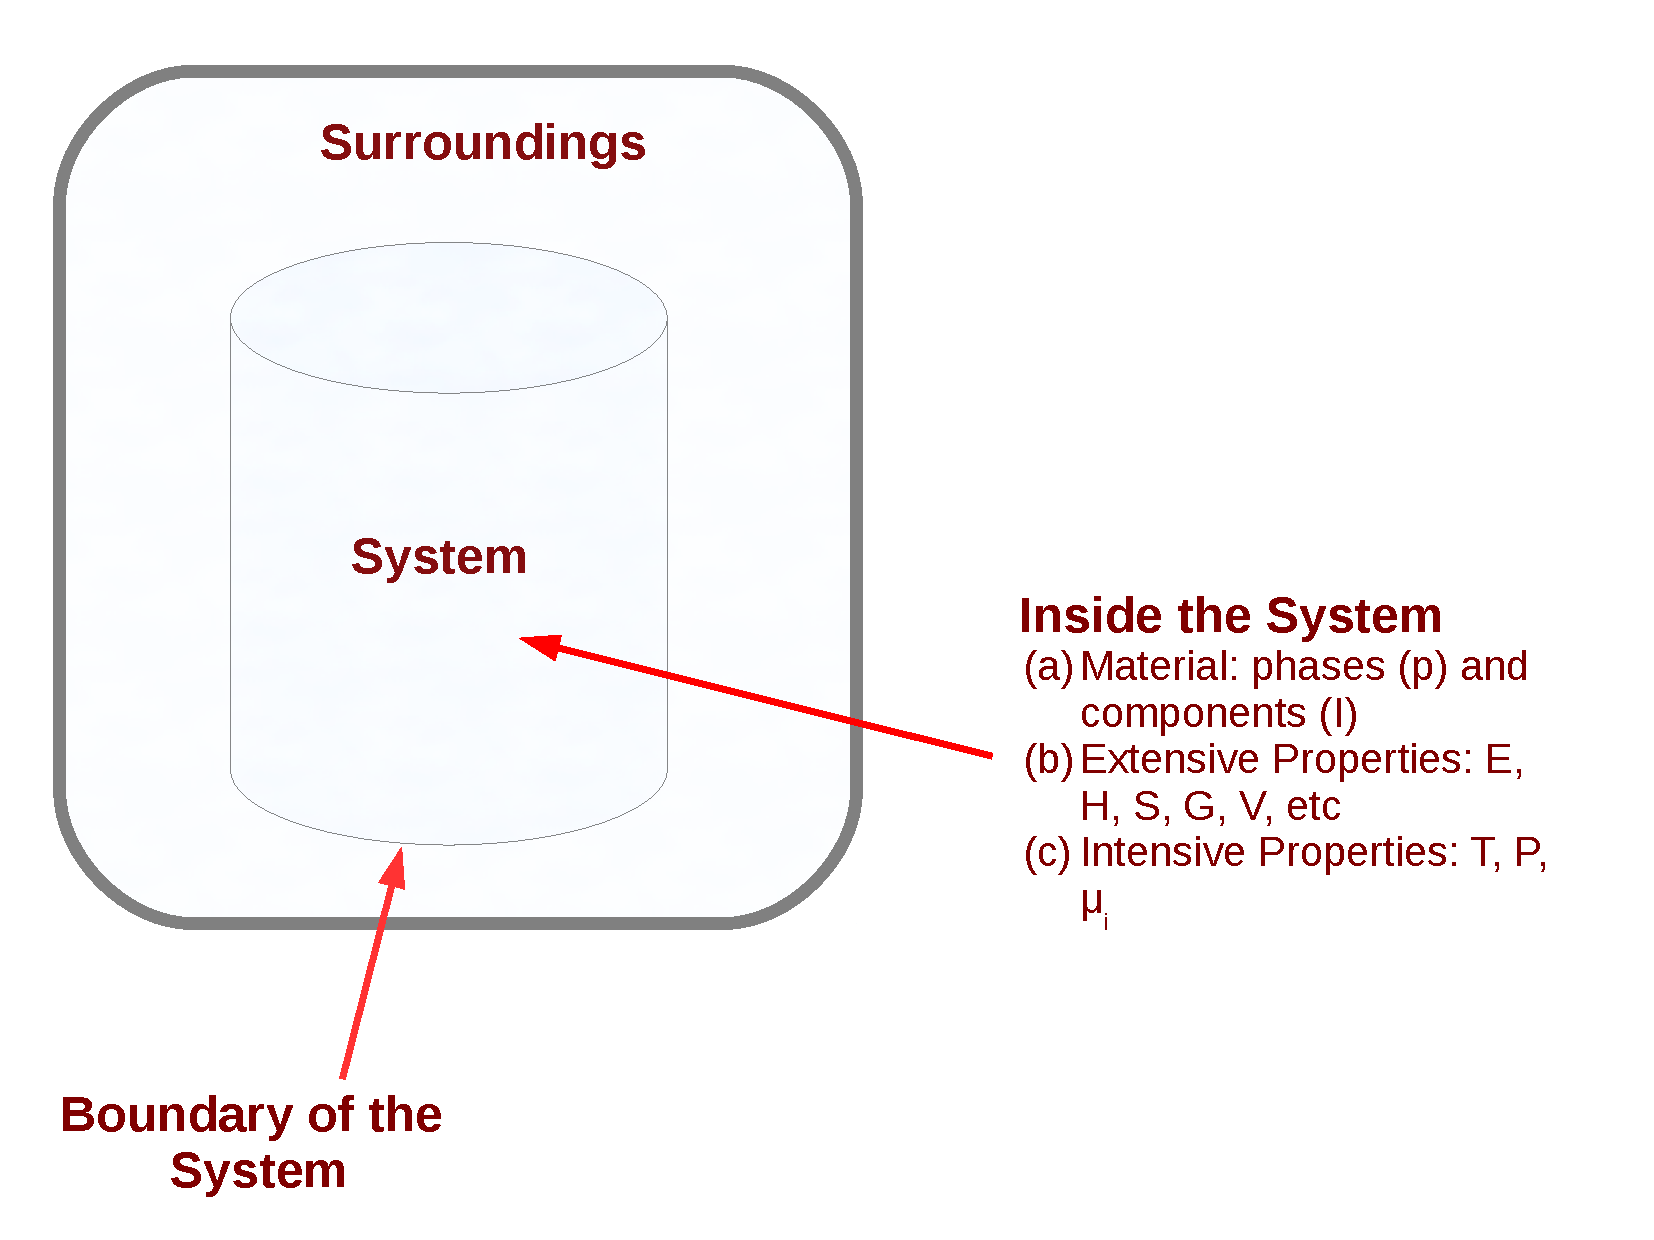
\includegraphics[width=\columnwidth,clip]{./../Pics/Fig_SystemDefinition}
        \end{center}
      \end{figure}
      \begin{tabular}{|c|c|c|}
         \hline
                      & {\bf Mass} & {\bf Energy} \\
                      & {\bf Exchange} & {\bf Exchange} \\
         \hline
         {\bf Open}   & {\it yes}  & {\it yes}    \\
         {\bf Closed} & {\it no}   & {\it yes}    \\
         {\bf Isolated}&{\it no}   & {\it no}     \\
         \hline 
      \end{tabular}    
    \end{column}
  \end{columns}
\end{frame}
\normalsize



%%%
%%% Slide
%%%
\begin{frame}
 \frametitle{System and Control Volumes}
  \begin{columns}
    \begin{column}[l]{0.6\linewidth}
      \begin{enumerate}\setcounter{enumi}{8}\scriptsize
         \item <1-> The \textcolor{red}{material} in a system is composed of phases (e.g., solid, liquid, gas) with distinct physical and chemical properties;
         \item <2-> The \textcolor{red}{composition} of each phase is described by a series of discrete chemical formula units (i.e., chemical components) -- e.g., water/steam $\left(\right.$H$_{2}$O$\left.\right)$, ammonia $\left(\right.$NH$_{3}\left.\right)$, carbon dioxide $\left(\right.$CO$_{2}\left.\right)$, etc;
         \item <3-> Any characteristic of a system is called a \textcolor{red}{property} -- e.g., pressure, temperature, mass, etc;
         \item <4-> Properties can be classified as \textcolor{red}{intensive} or \textcolor{red}{extensive};
         \item <5-> \textcolor{red}{Intensive properties} are those that are {\bf independent} of the mass of a system -- e.g., temperature, pressure, density, viscosity, etc;
         \item <6-> \textcolor{red}{Extensive properties} are those whose values {\bf depend} on the size (or extent) of the system -- e.g., mass, volume, number of moles, internal energy, enthalpy, entropy, etc.  
      \end{enumerate} 
    \end{column}
    \begin{column}[l]{0.4\linewidth}\scriptsize
      \begin{figure}%
        \begin{center}
          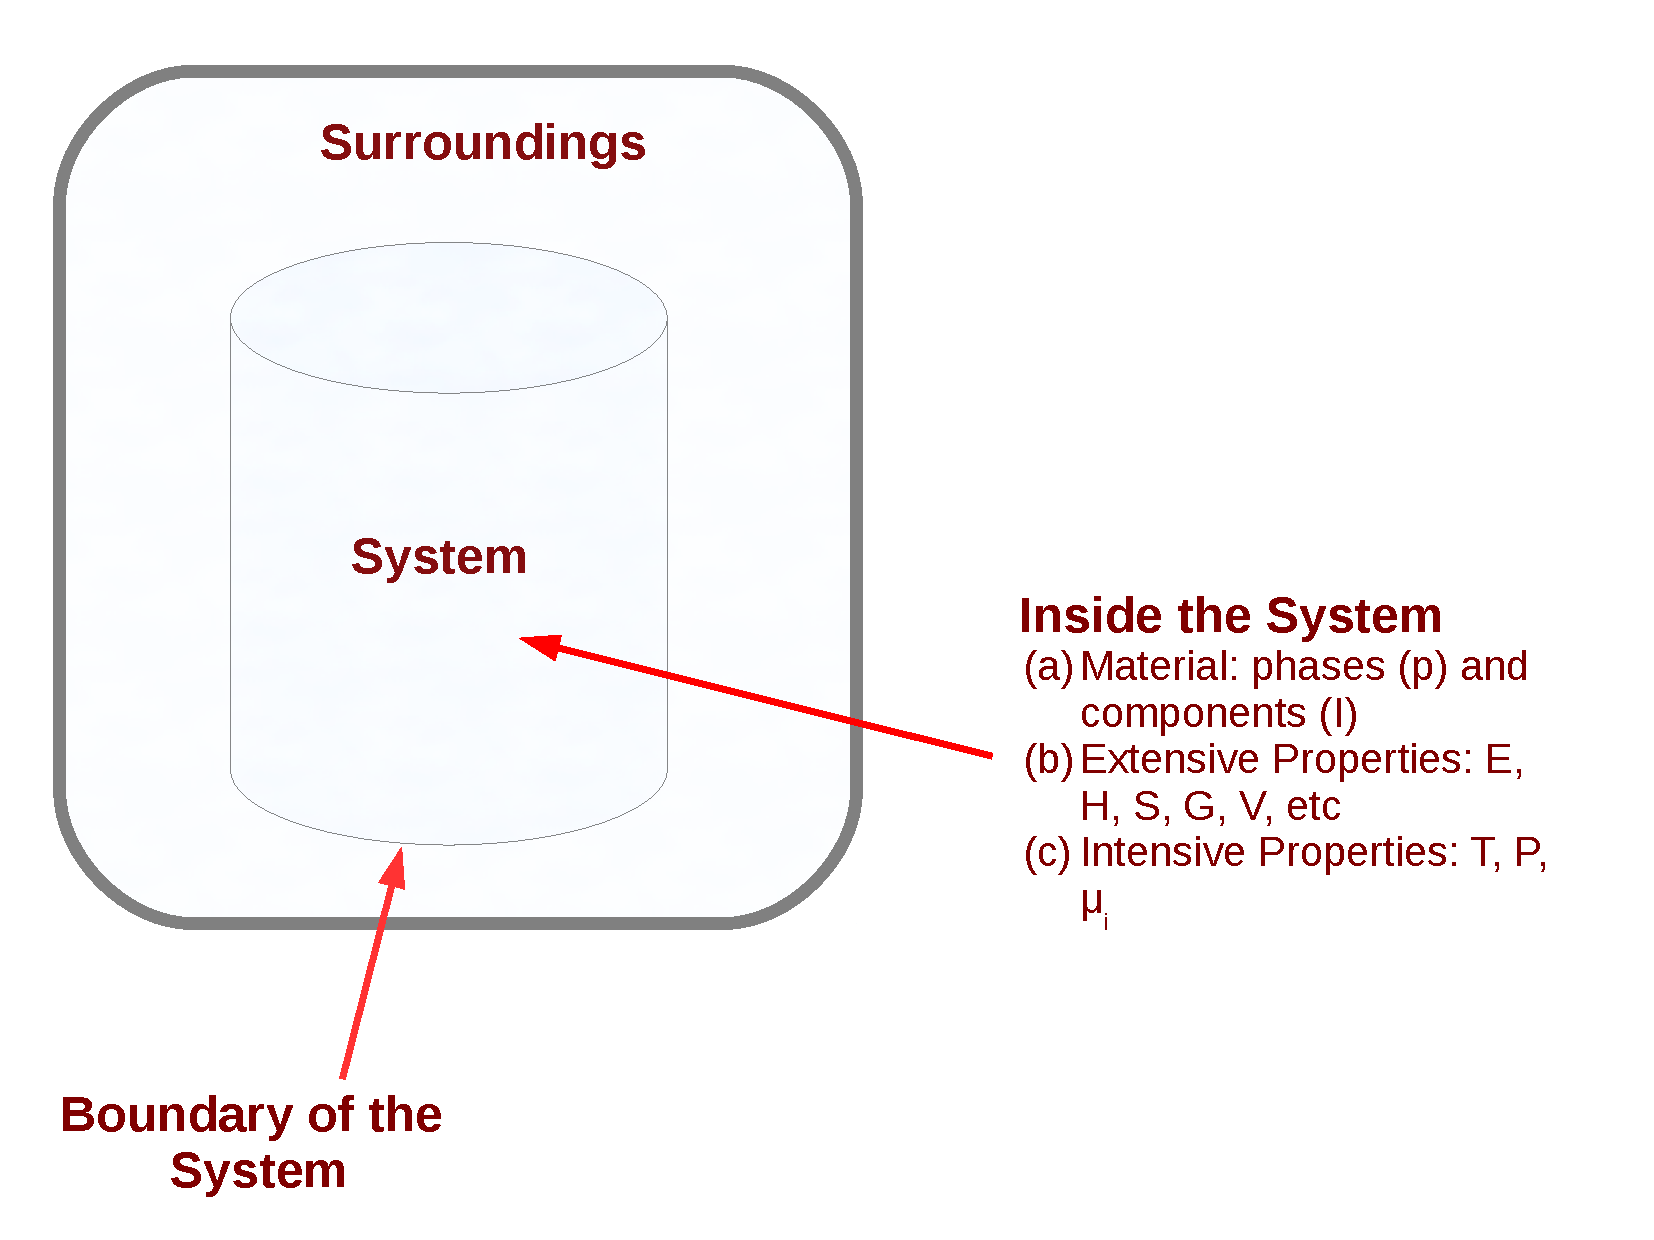
\includegraphics[width=\columnwidth,clip]{./../Pics/Fig_SystemDefinition}
        \end{center}
      \end{figure}
      \begin{tabular}{|c|c|c|}
         \hline
                      & {\bf Mass} & {\bf Energy} \\
                      & {\bf Exchange} & {\bf Exchange} \\
         \hline
         {\bf Open}   & {\it yes}  & {\it yes}    \\
         {\bf Closed} & {\it no}   & {\it yes}    \\
         {\bf Isolated}&{\it no}   & {\it no}     \\
         \hline 
      \end{tabular}    
    \end{column}
  \end{columns}
\end{frame}


\begin{comment}

%%%
%%% SECTION
%%%
\section{Review of the Main Tools for the Course}


%%%
%%% SUBSECTION
%%%
\subsection{PVT Relations}

%%%
%%% Slide
%%%
\begin{frame}
 \frametitle{PVT Behaviour of Pure Substances}
 \begin{columns}
  \begin{column}[l]{0.5\linewidth}
    \begin{enumerate}\scriptsize
    \item <1-> This surface represents the \textcolor{red}{Pressure} - \textcolor{red}{specific volume} - \textcolor{red}{Temperature} -- $PVT$, relation in a pure substance;
    \item <2-> Any given coordinate in both, the surface plot and diagrams (projections), will represent values of pressure, specific volume and temperature when the substance is at equilibrium;
    \item <3-> The \textcolor{red}{Gibbs phase rule},
       \visible<3->{\begin{equation}
          \Psi = 2 + \mathcal{C} - \mathcal{P}
       \end{equation} 
       describes the number of degrees of freedom (dof), $\Psi$ (\underline{intensive variables}, e.g., temperature, pressure), in a closed system at equilibrium as a function of the number of phases ($\mathcal{P}$ = solid, liquid and vapour) and components, $\mathcal{C}$ (e.g., water, CO$_{2}$, N$_{2}$, etc). }
\end{enumerate}
  \end{column}
  \begin{column}[l]{0.5\linewidth}
   \begin{figure}%
    \begin{center}
     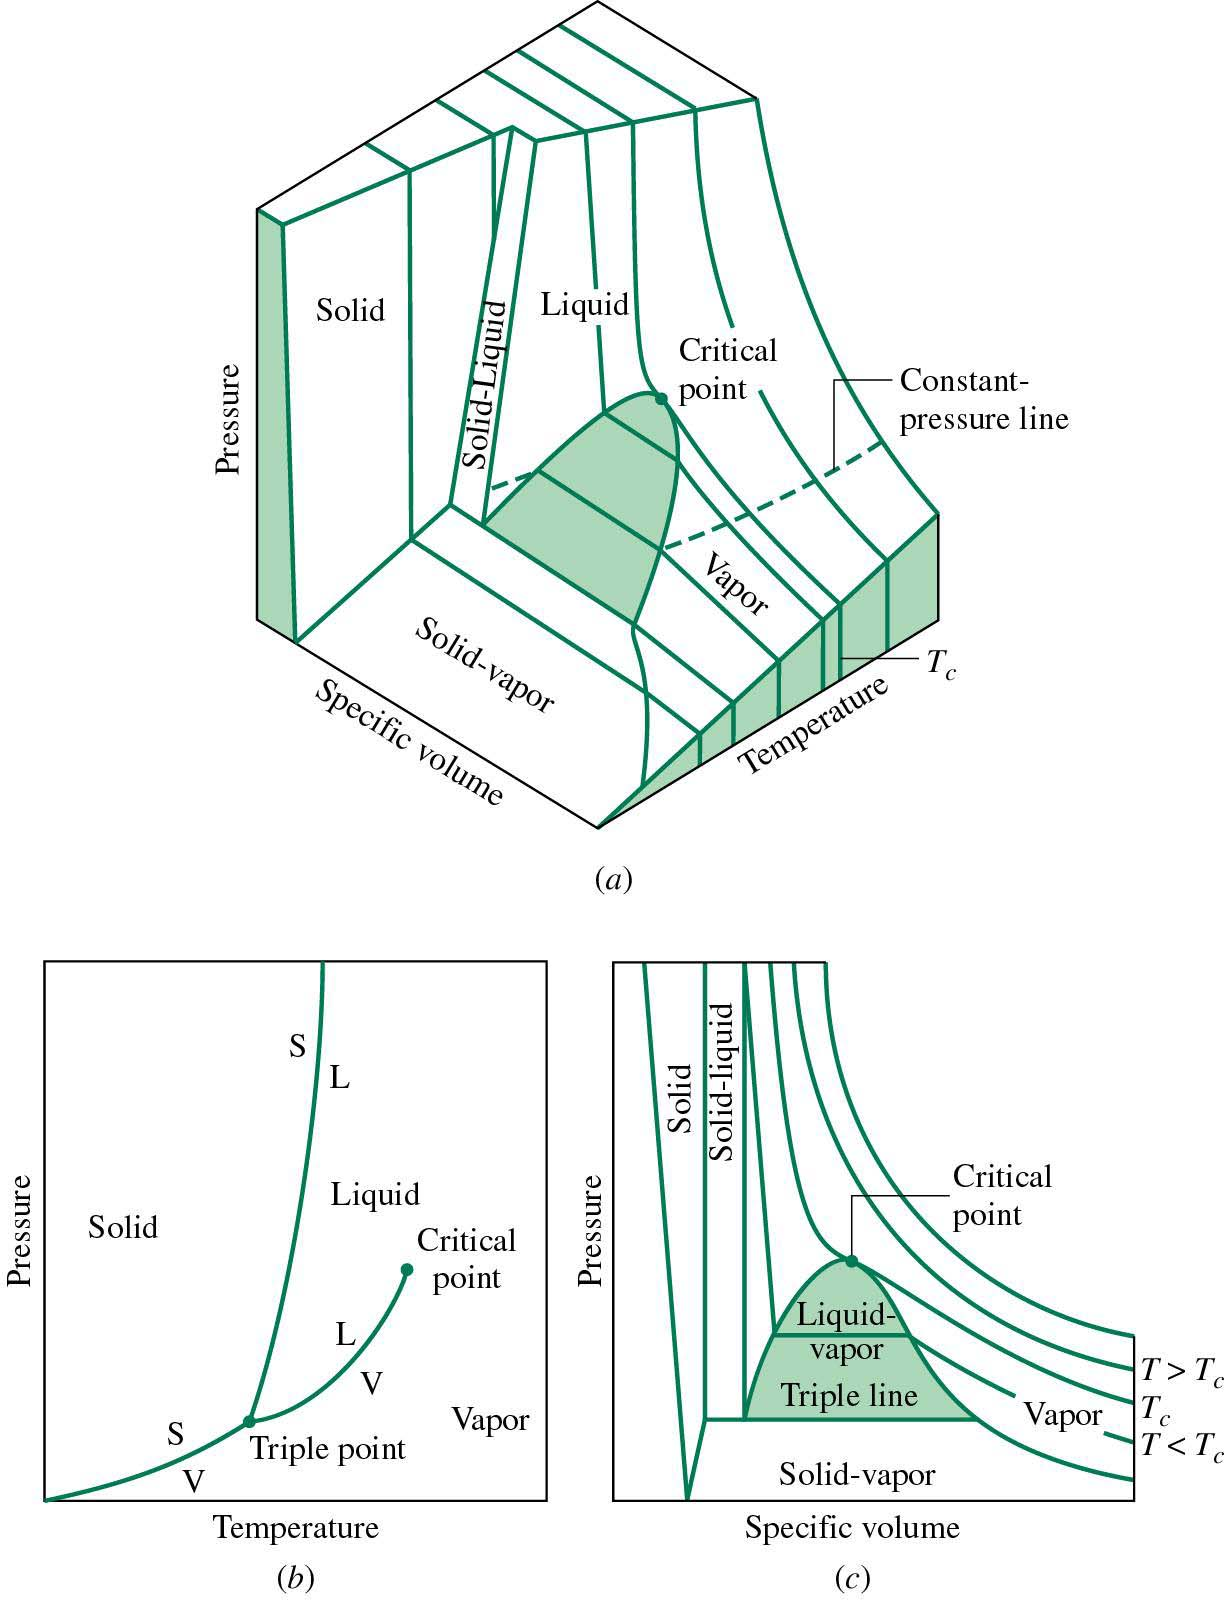
\includegraphics[width=4.cm,clip]{./../Pics/PVT_Surface.jpg}
    \end{center}
    \scriptsize\caption{\scriptsize$PVT$ surface (top) and projections onto (b) $PT$ and (c) $PV$ diagrams for a pure substance (Extracted from [4]).}
   \end{figure}    
  \end{column}
 \end{columns}
\end{frame}

%%%
%%% Slide
%%%
\begin{frame}
 \frametitle{PVT Behaviour of Pure Substances}
 \begin{columns}
   \begin{column}[l]{0.5\linewidth}
     \begin{enumerate}\setcounter{enumi}{3}\scriptsize
        \item <1-> {\bf Example 1:} In the $PT$ diagram (b) for one hypothetical component -- $\textcolor{red}{\mathcal{C}=1}$, within each phase region -- $\textcolor{blue}{\mathcal{P}=1}$ (i.e., as either solid, liquid or vapour phases),
          \visible<1->{\begin{displaymath}
            \Psi = 2 + \textcolor{red}{1} - \textcolor{blue}{1} = 2
          \end{displaymath}
          \begin{enumerate}[(a)]\scriptsize
             \item  In this case, the number of degrees of freedom correspond to temperature and pressure;
             \item  Thus, within the vapour phase, temperature and pressure can readily be changed without explicit phase change or composition of the vapour phase.
          \end{enumerate}}
        \item <2-> {\bf Example 2:} However, along with the \textcolor{red}{phase-line boundary}, two phases are in equilibrium, i.e., $\textcolor{blue}{\mathcal{P}=2}$,%
          \visible<2->{\begin{displaymath}
            \Psi = 2 + \textcolor{red}{1} - \textcolor{blue}{2} = 1
          \end{displaymath}
          When the vapour and liquid phases are in equilibrium, any change in temperature {\bf leads} to change in pressure for the system remains in equilibrium;}
     \end{enumerate}
  \end{column}
  \begin{column}[l]{0.5\linewidth}
   \begin{figure}%
    \begin{center}
     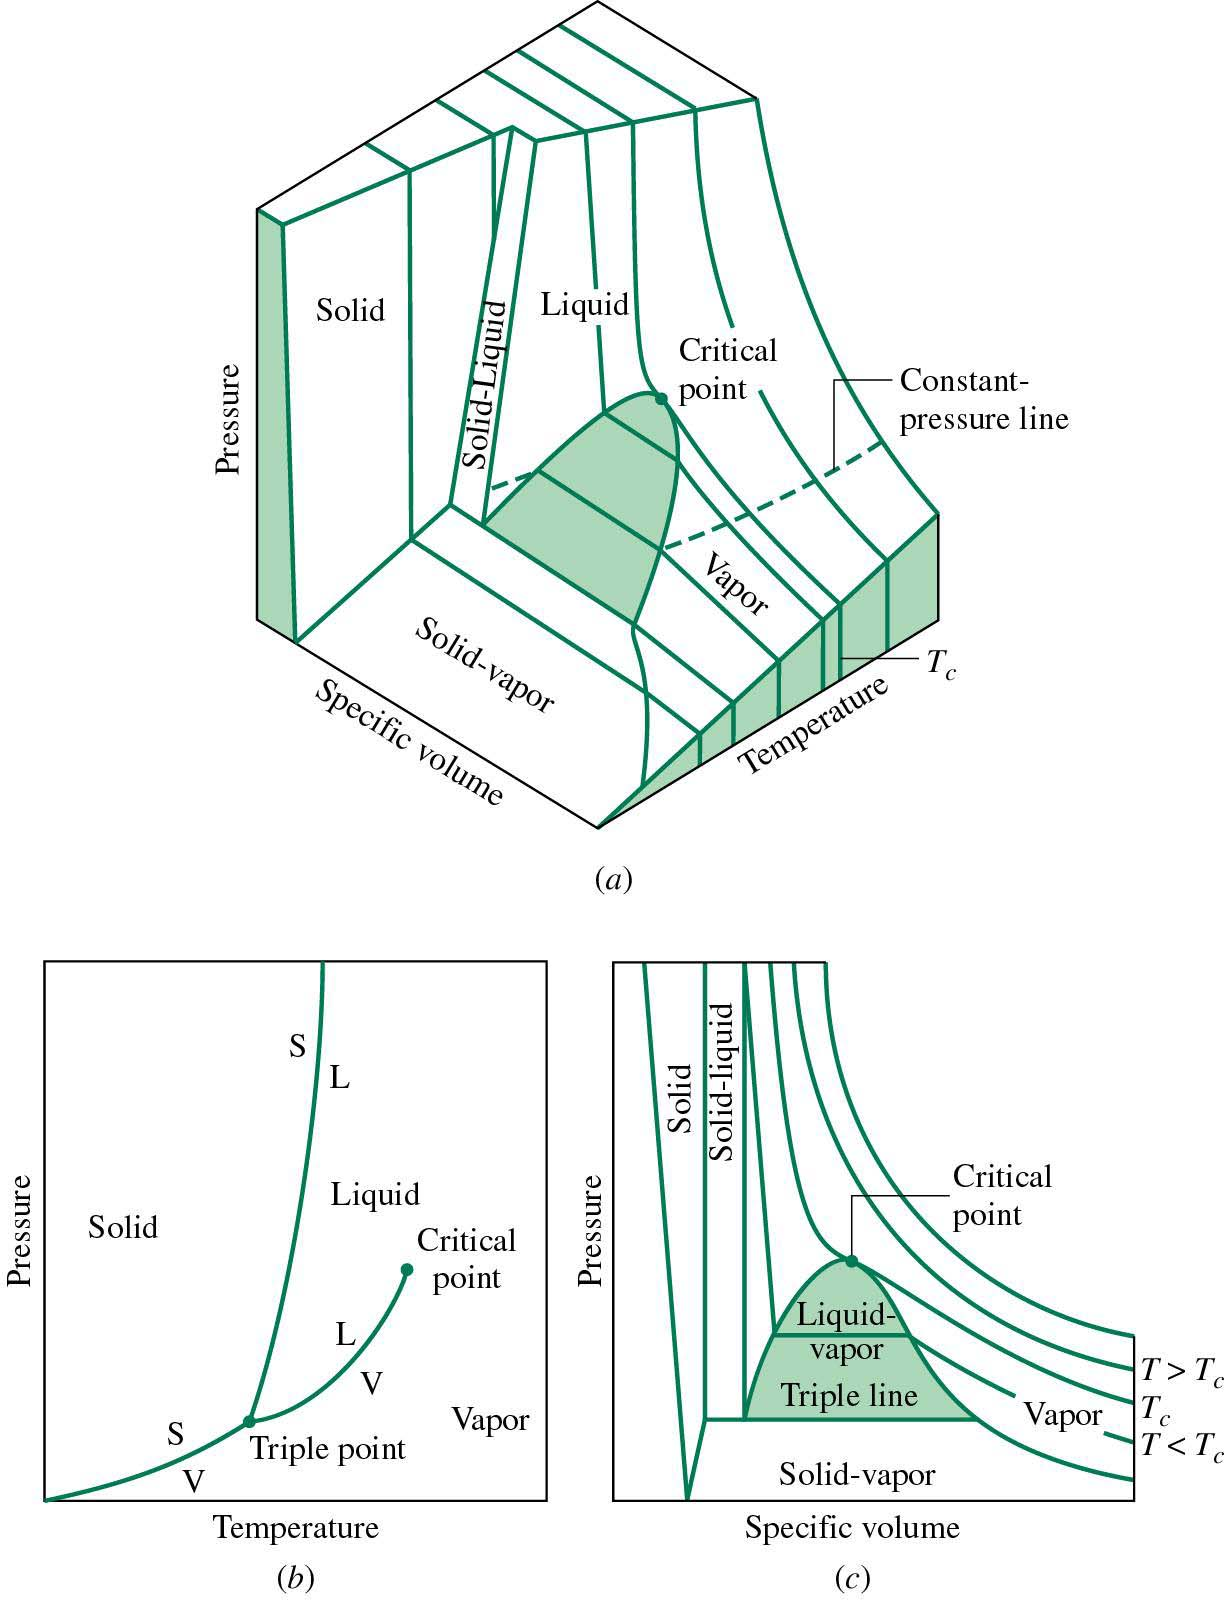
\includegraphics[width=4.cm,clip]{./../Pics/PVT_Surface.jpg}
    \end{center}
    \scriptsize\caption{\scriptsize$PVT$ surface (top) and projections onto (b) $PT$ and (c) $PV$ diagrams for a pure substance (Extracted from [4]).}
   \end{figure}    
  \end{column}
 \end{columns}
\end{frame}
 

%%%
%%% Slide
%%%
\begin{frame}
 \frametitle{PVT Behaviour of Pure Substances}
 \begin{columns}
    \begin{column}[l]{0.5\linewidth}
      \begin{enumerate}\setcounter{enumi}{5}\scriptsize
         \item <1-> {\bf Example 3:} Similarly, for the \textcolor{blue}{\underline{\bf triple point}} -- $\textcolor{blue}{\mathcal{P}=3}$, all three phases are in equilibrium
           \visible<1->{\begin{displaymath}
             \Psi = 2 + \textcolor{red}{1} - \textcolor{blue}{3} = 0
           \end{displaymath}}
           \begin{enumerate}[(a)]\scriptsize
              \item <1-> Here there is {\bf no degrees of freedom} -- i.e., there is {\bf just} one value for pressure and temperature that make the {\bf three phases to coexist}.
              \item <2-> Any change in either intensive properties will drive the system away from the {\it triple point}.
           \end{enumerate}
     \end{enumerate}
  \end{column}
  \begin{column}[l]{0.5\linewidth}
   \begin{figure}%
    \begin{center}
     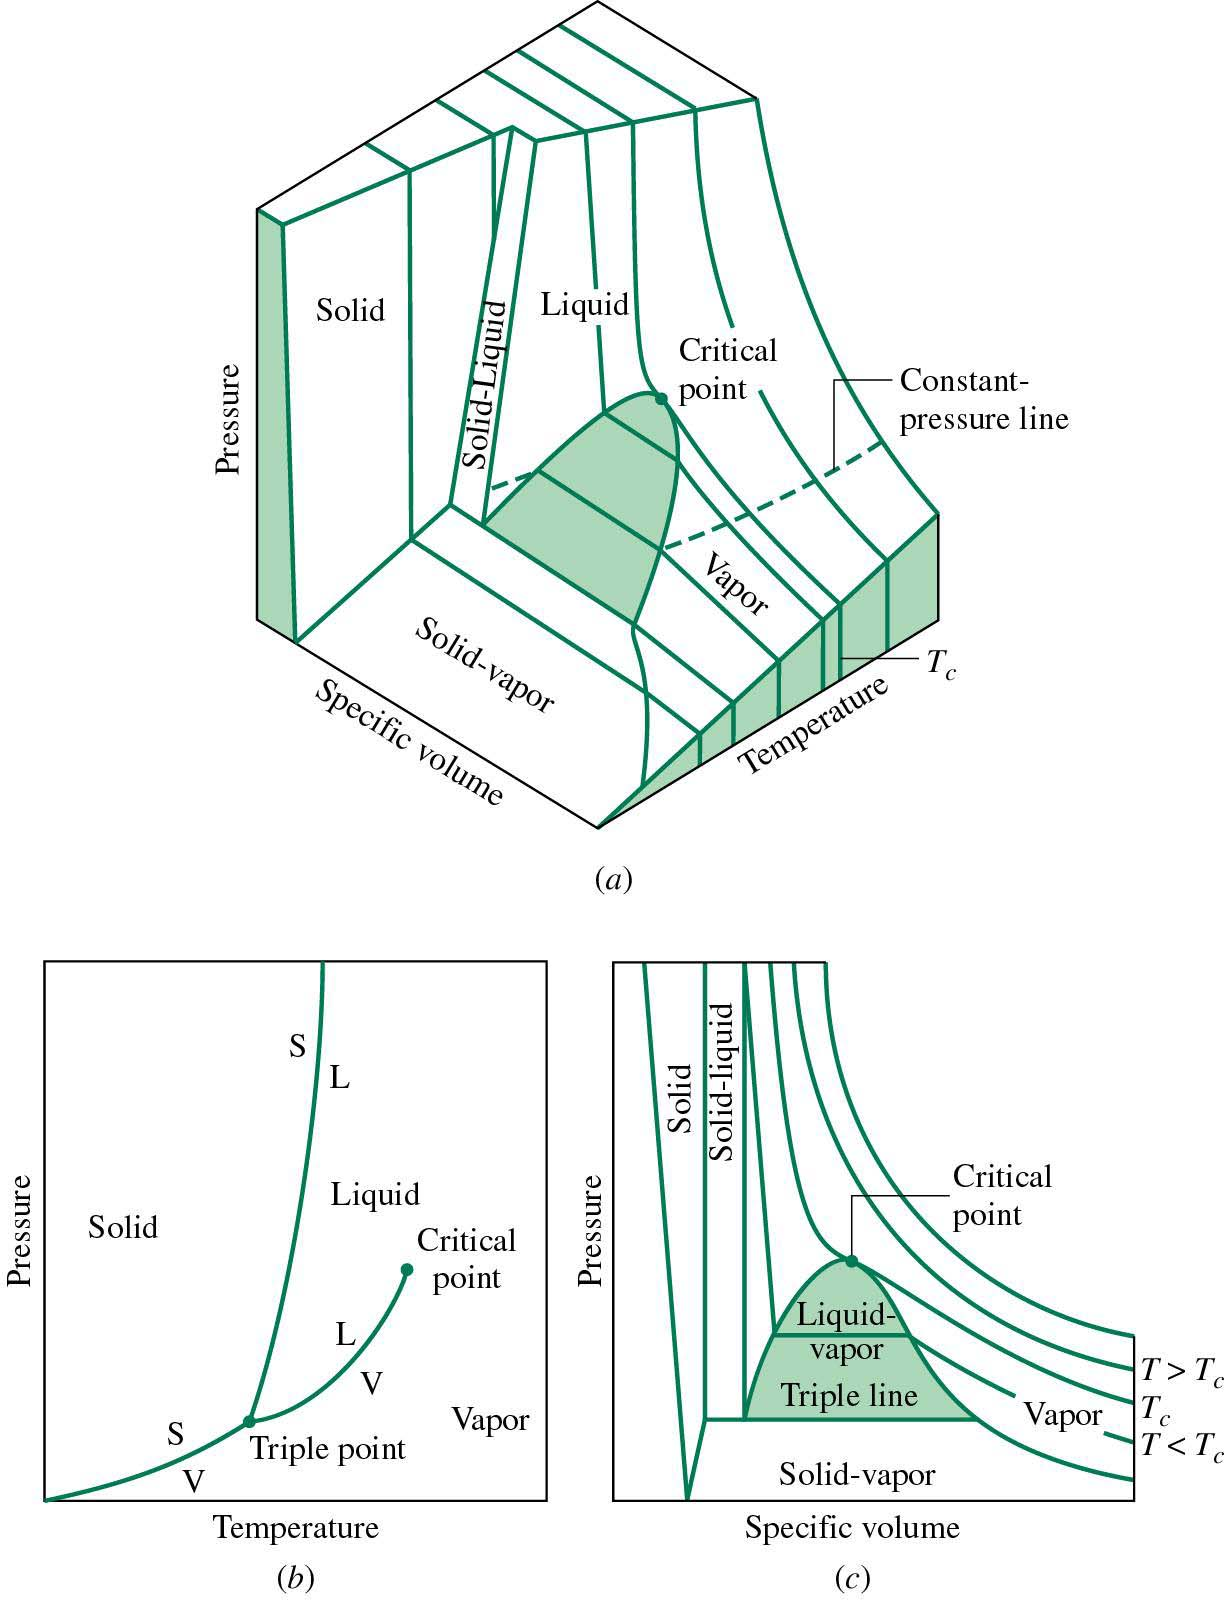
\includegraphics[width=4.cm,clip]{./../Pics/PVT_Surface.jpg}
    \end{center}
    \scriptsize\caption{\scriptsize$PVT$ surface (top) and projections onto (b) $PT$ and (c) $PV$ diagrams for a pure substance (Extracted from [4]).}
   \end{figure}    
  \end{column}
 \end{columns}
\end{frame}


%%%
%%% SUBSECTION
%%%
\subsection{Thermodynamics Diagrams and Tables}

%%%
%%% Slide 
%%%
\begin{frame}
 \frametitle{Thermodynamics Diagrams: Pressure $\times$ Specific Enthalpy $(Ph)$ for CO$_{2}$}
  \begin{center}
   \begin{figure}
     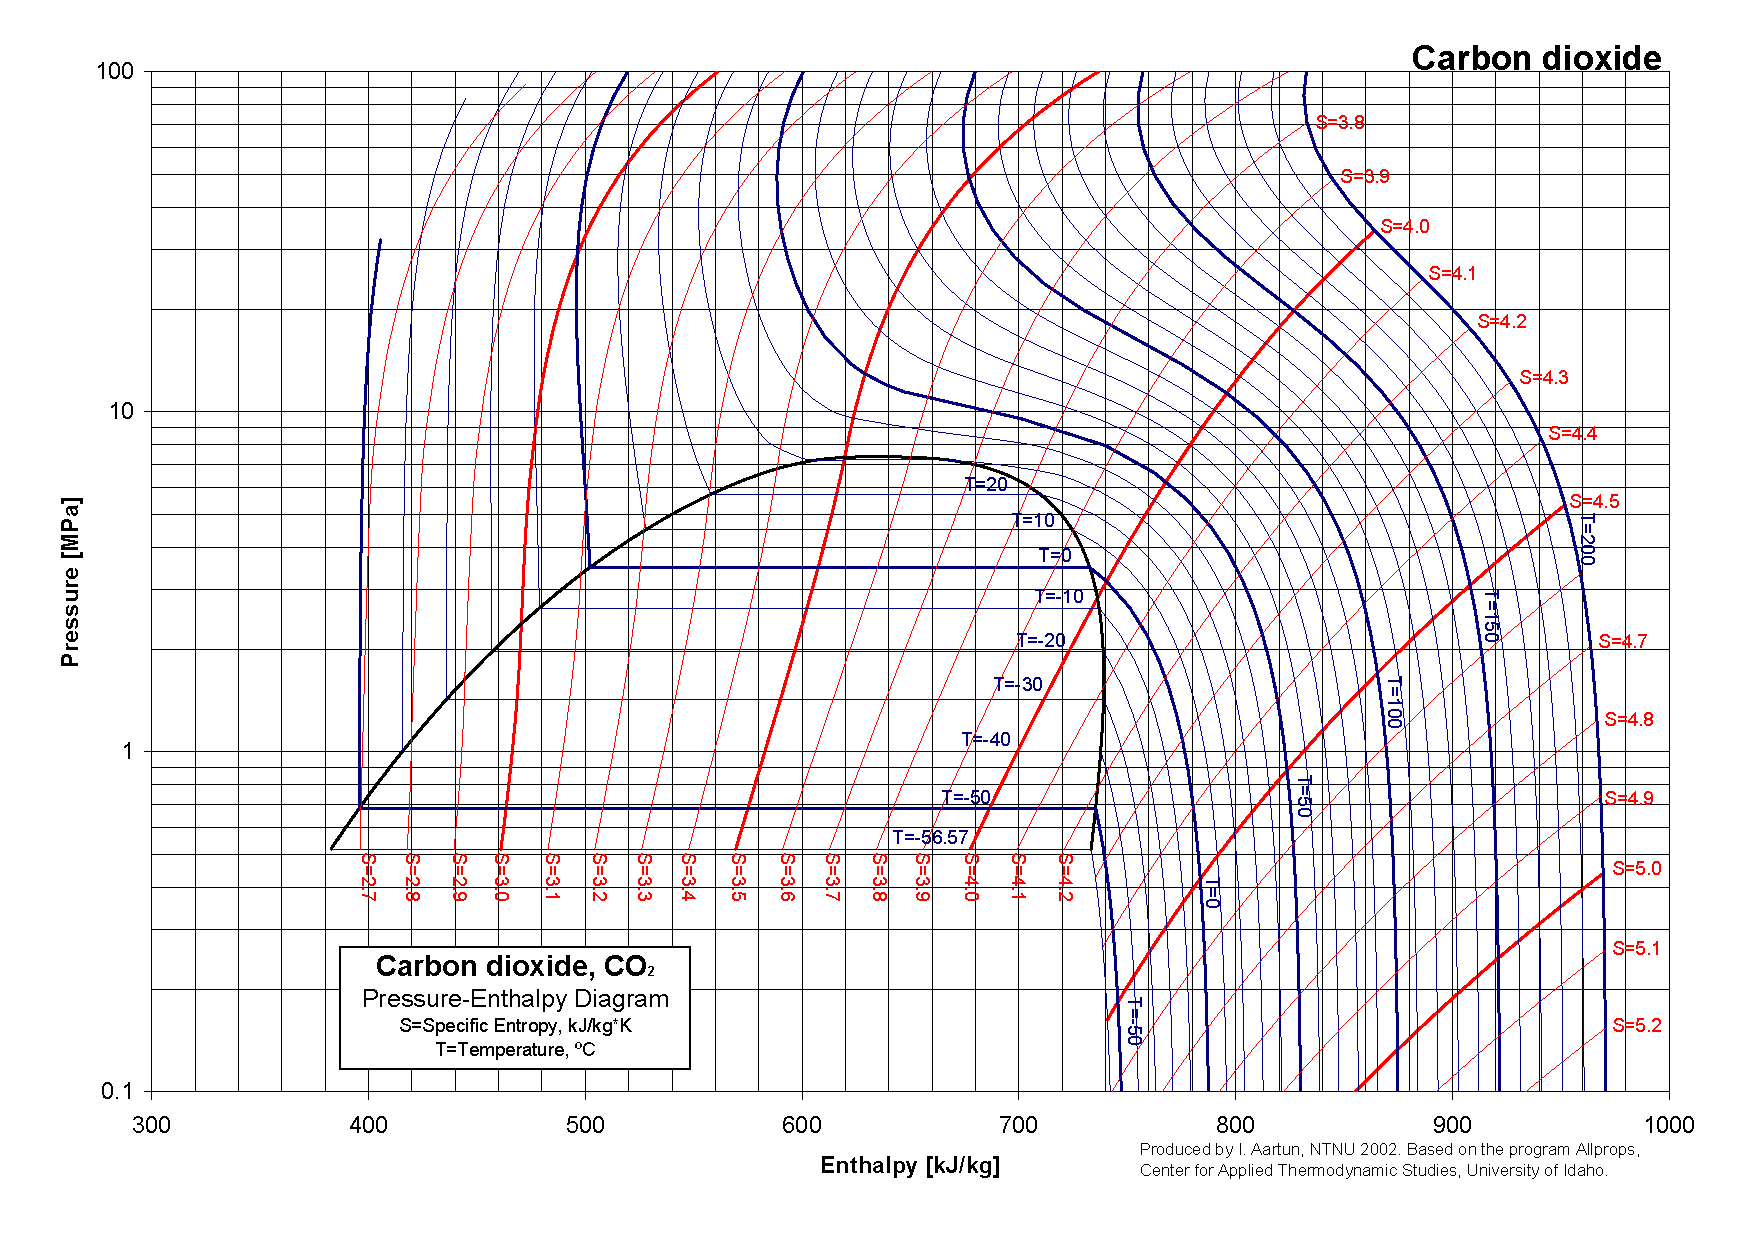
\includegraphics[width=8cm,height=7.cm,clip]{./../Pics/CO2col}
   \end{figure}
   \end{center}
\end{frame}

%%%
%%% Slide
%%%
\begin{frame}
 \frametitle{Thermodynamics Diagrams: Pressure $\times$ Specific Enthalpy $(Ph)$}
  \begin{center}
   \begin{figure}
      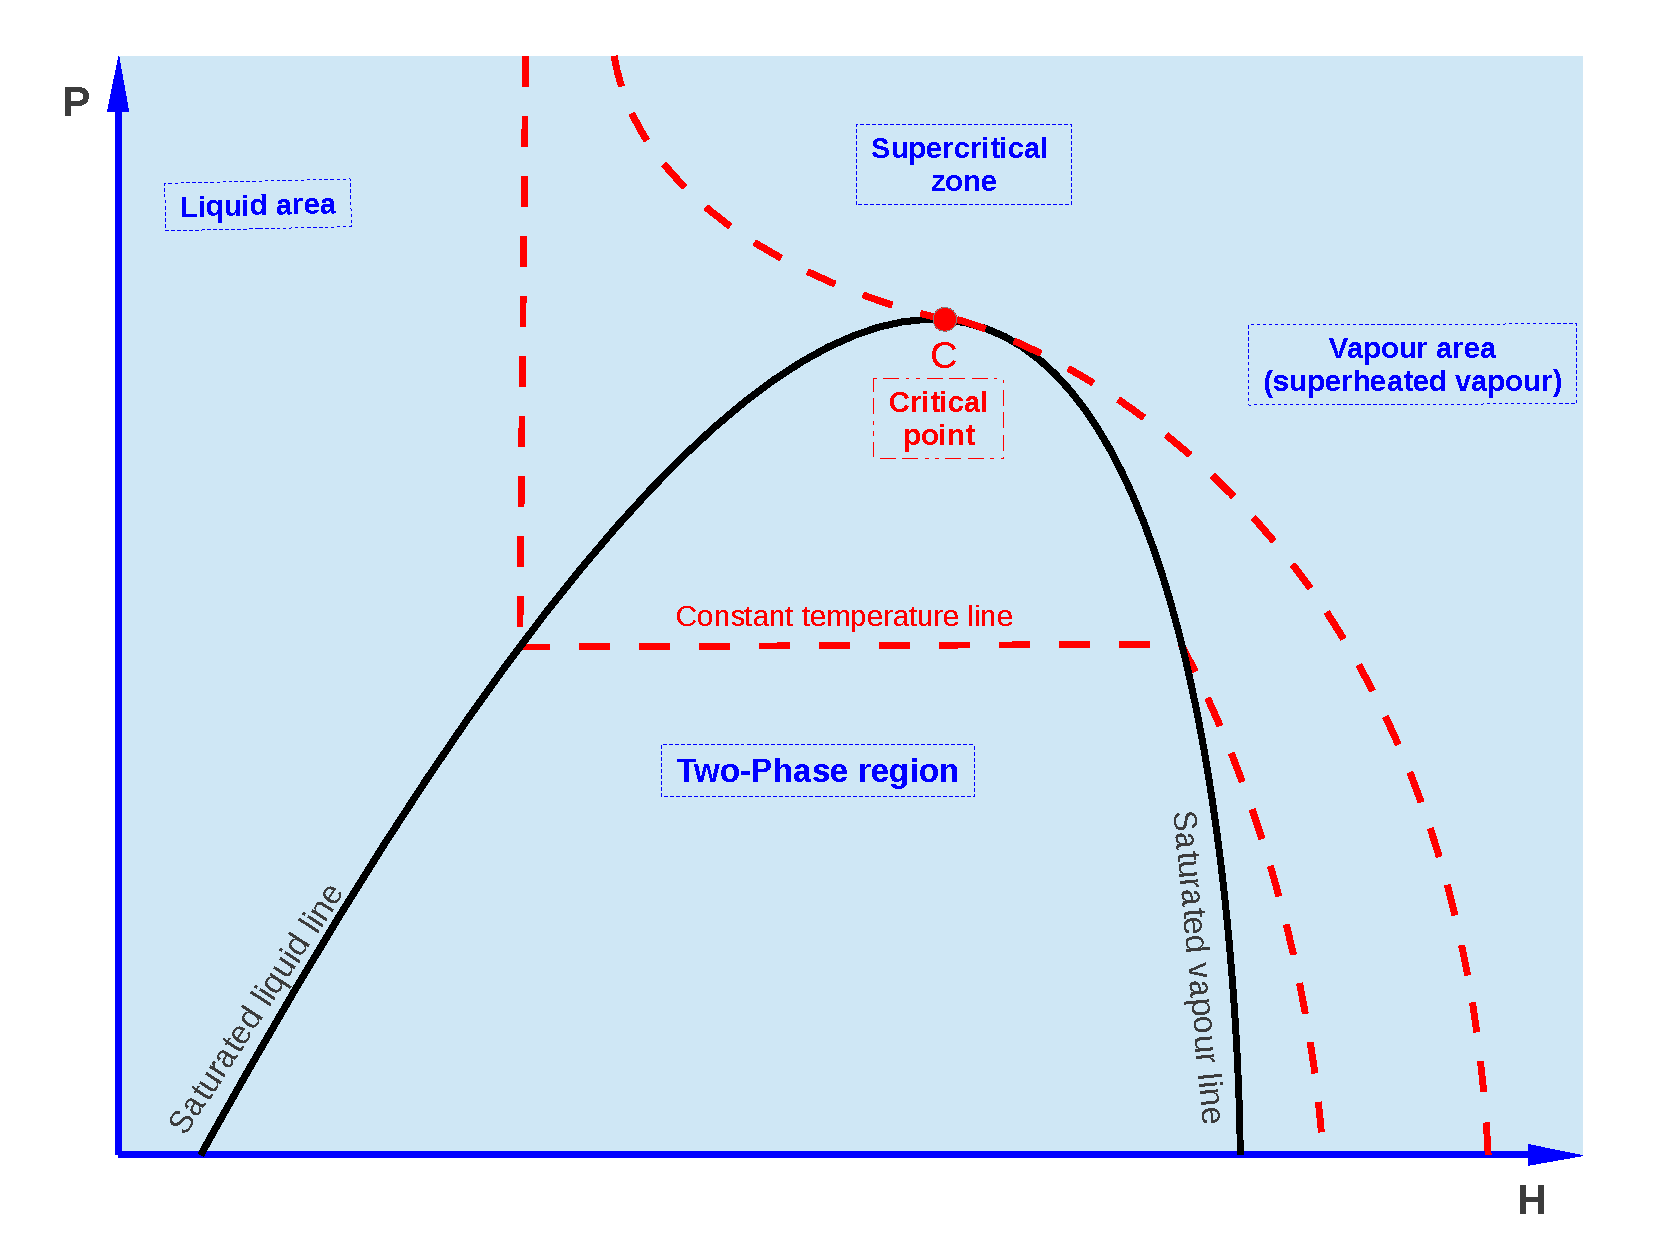
\includegraphics[width=8cm,height=7.cm,clip]{./../Pics/Overview_Refrig18}
   \end{figure}
   \end{center}
\end{frame}

%%%
%%% Slide
%%%
\begin{frame}
 \frametitle{Thermodynamics Diagrams: Pressure $\times$ Specific Enthalpy $(Ph)$}
  \begin{center}
   \begin{figure}
      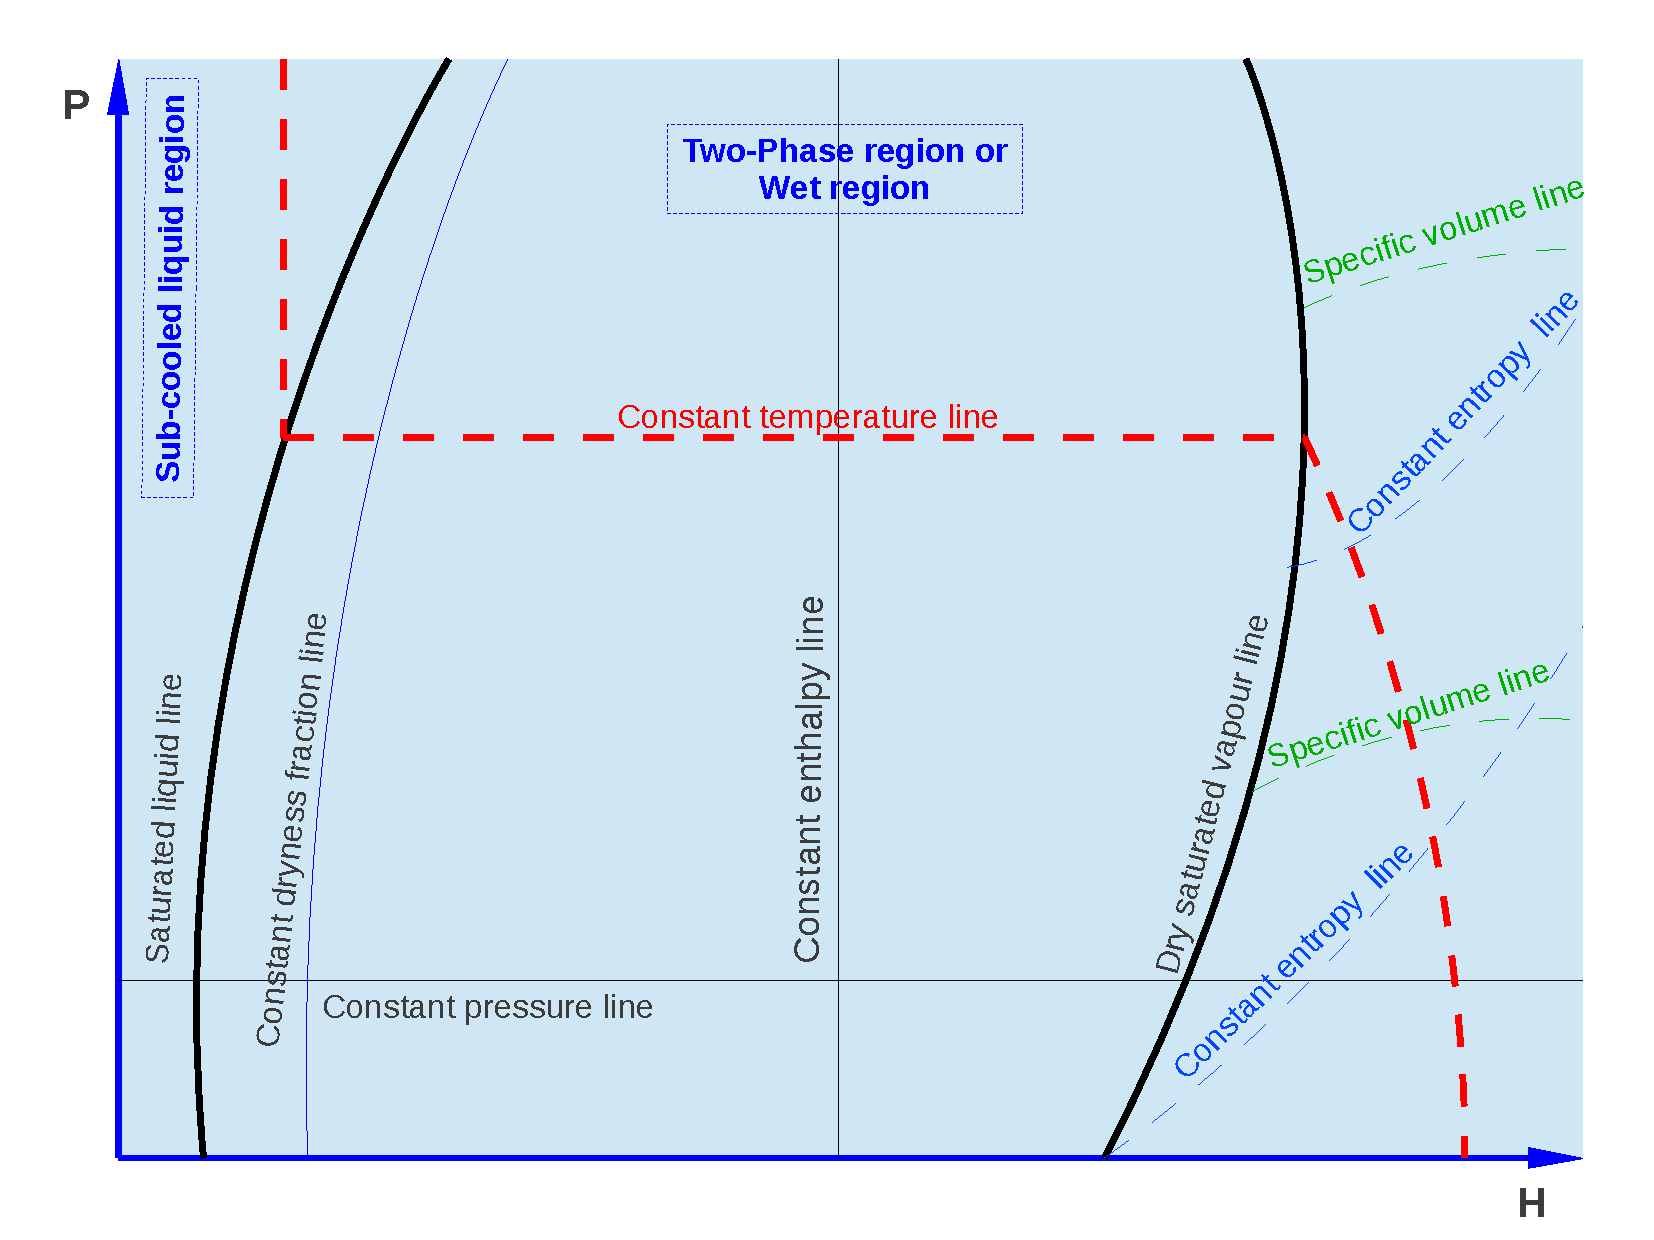
\includegraphics[width=8cm,height=7.cm,clip]{./../Pics/Overview_Refrig17}
   \end{figure}
   \end{center}
\end{frame}

%%%
%%% Slide
%%%
\begin{frame}
 \frametitle{Thermodynamics Diagrams: Temperature $\times$ Specific Entropy $(Ts)$ for Water}
  \begin{center}
   \begin{figure}
     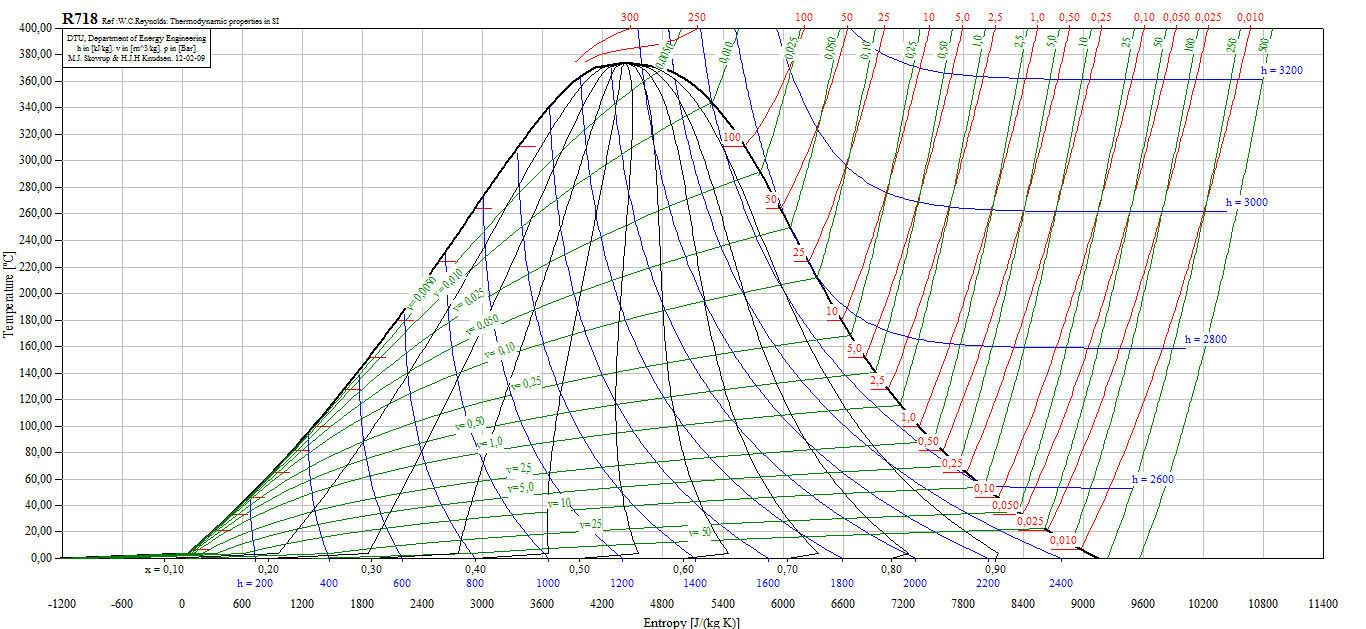
\includegraphics[width=8cm,height=7.cm,clip]{./../Pics/water_TS.png}
   \end{figure}
   \end{center}
\end{frame}

%%%
%%% Slide
%%%
\begin{frame}
 \frametitle{Thermodynamics Diagrams: Temperature $\times$ Specific Entropy $(Ts)$}
  \begin{center}
   \begin{figure}
      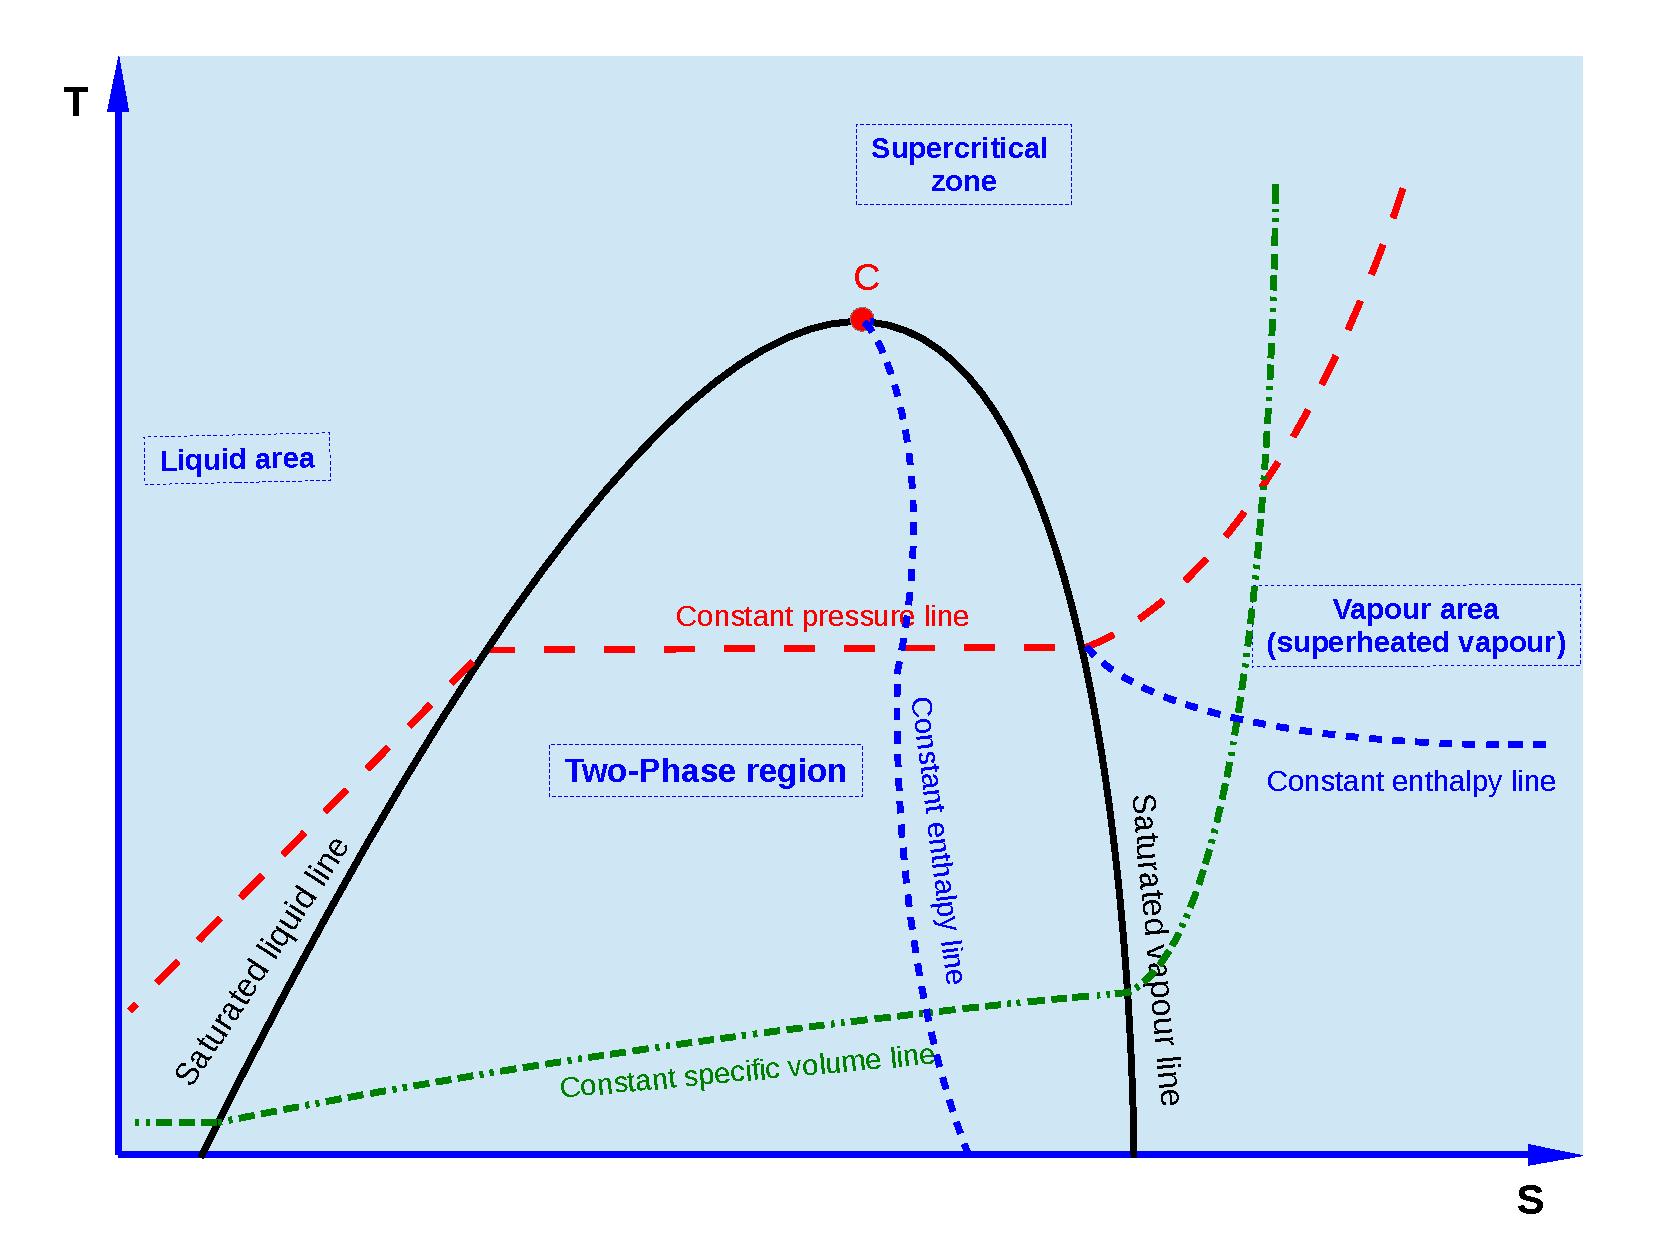
\includegraphics[width=8cm,height=7.cm,clip]{./../Pics/TS_Diag_Schematics}
   \end{figure}
   \end{center}
\end{frame}

%%%
%%% Slide
%%%
\begin{frame}
  \frametitle{Another option: (a) \red{Saturated} and (b) Superheated Tables with (c) Linear Interpolation}
\scriptsize{From Reference [4]:}\vspace{-.8cm}
   \begin{center}
   \begin{figure}
      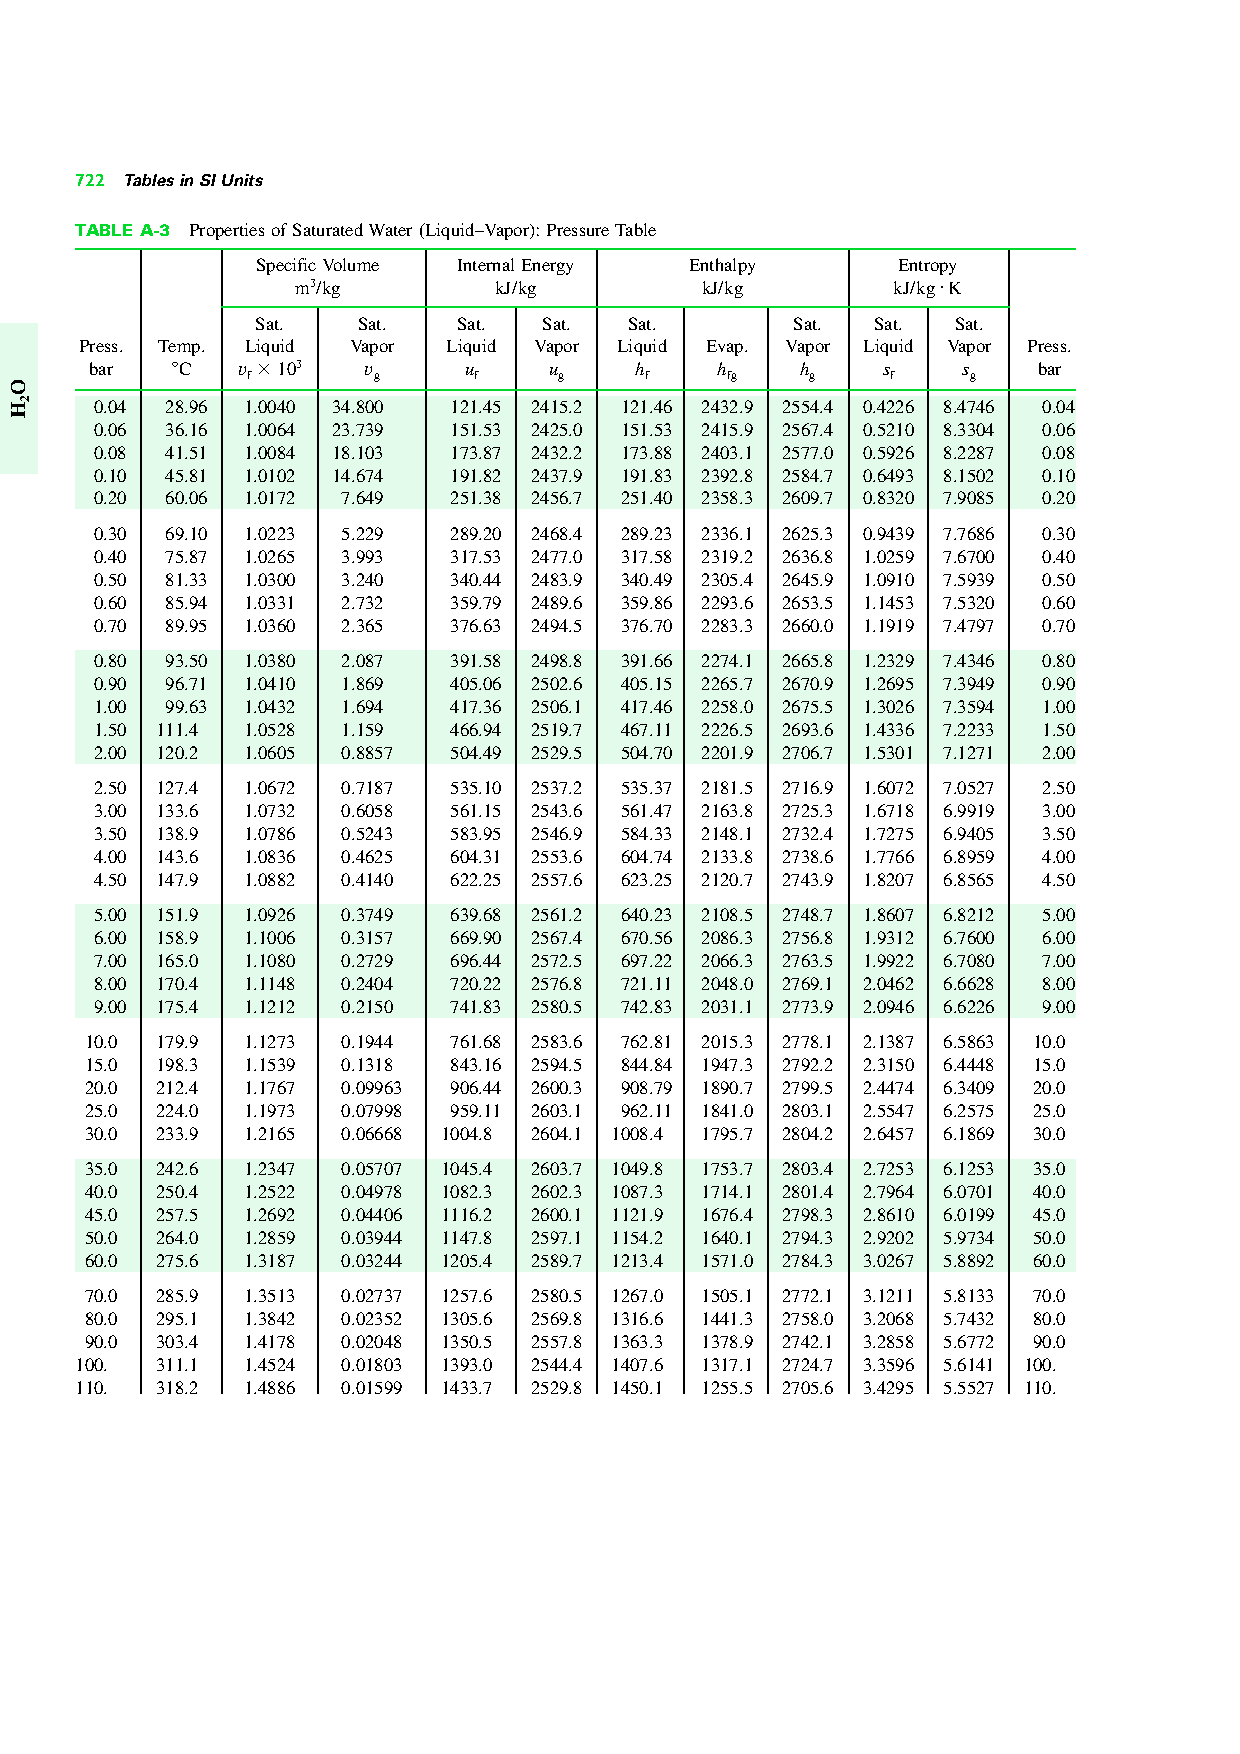
\includegraphics[width=9.cm,height=9.5cm,clip]{./../Pics/WaterSatTable}
   \end{figure}
   \end{center}
\end{frame}

%%%
%%% Slide
%%%
\begin{frame}
  \frametitle{Another option: (a) Saturated and (b) \red{Superheated Tables} with (c) Linear Interpolation}
\scriptsize{From Reference (d):}\vspace{-.8cm}
   \begin{center}
   \begin{figure}
      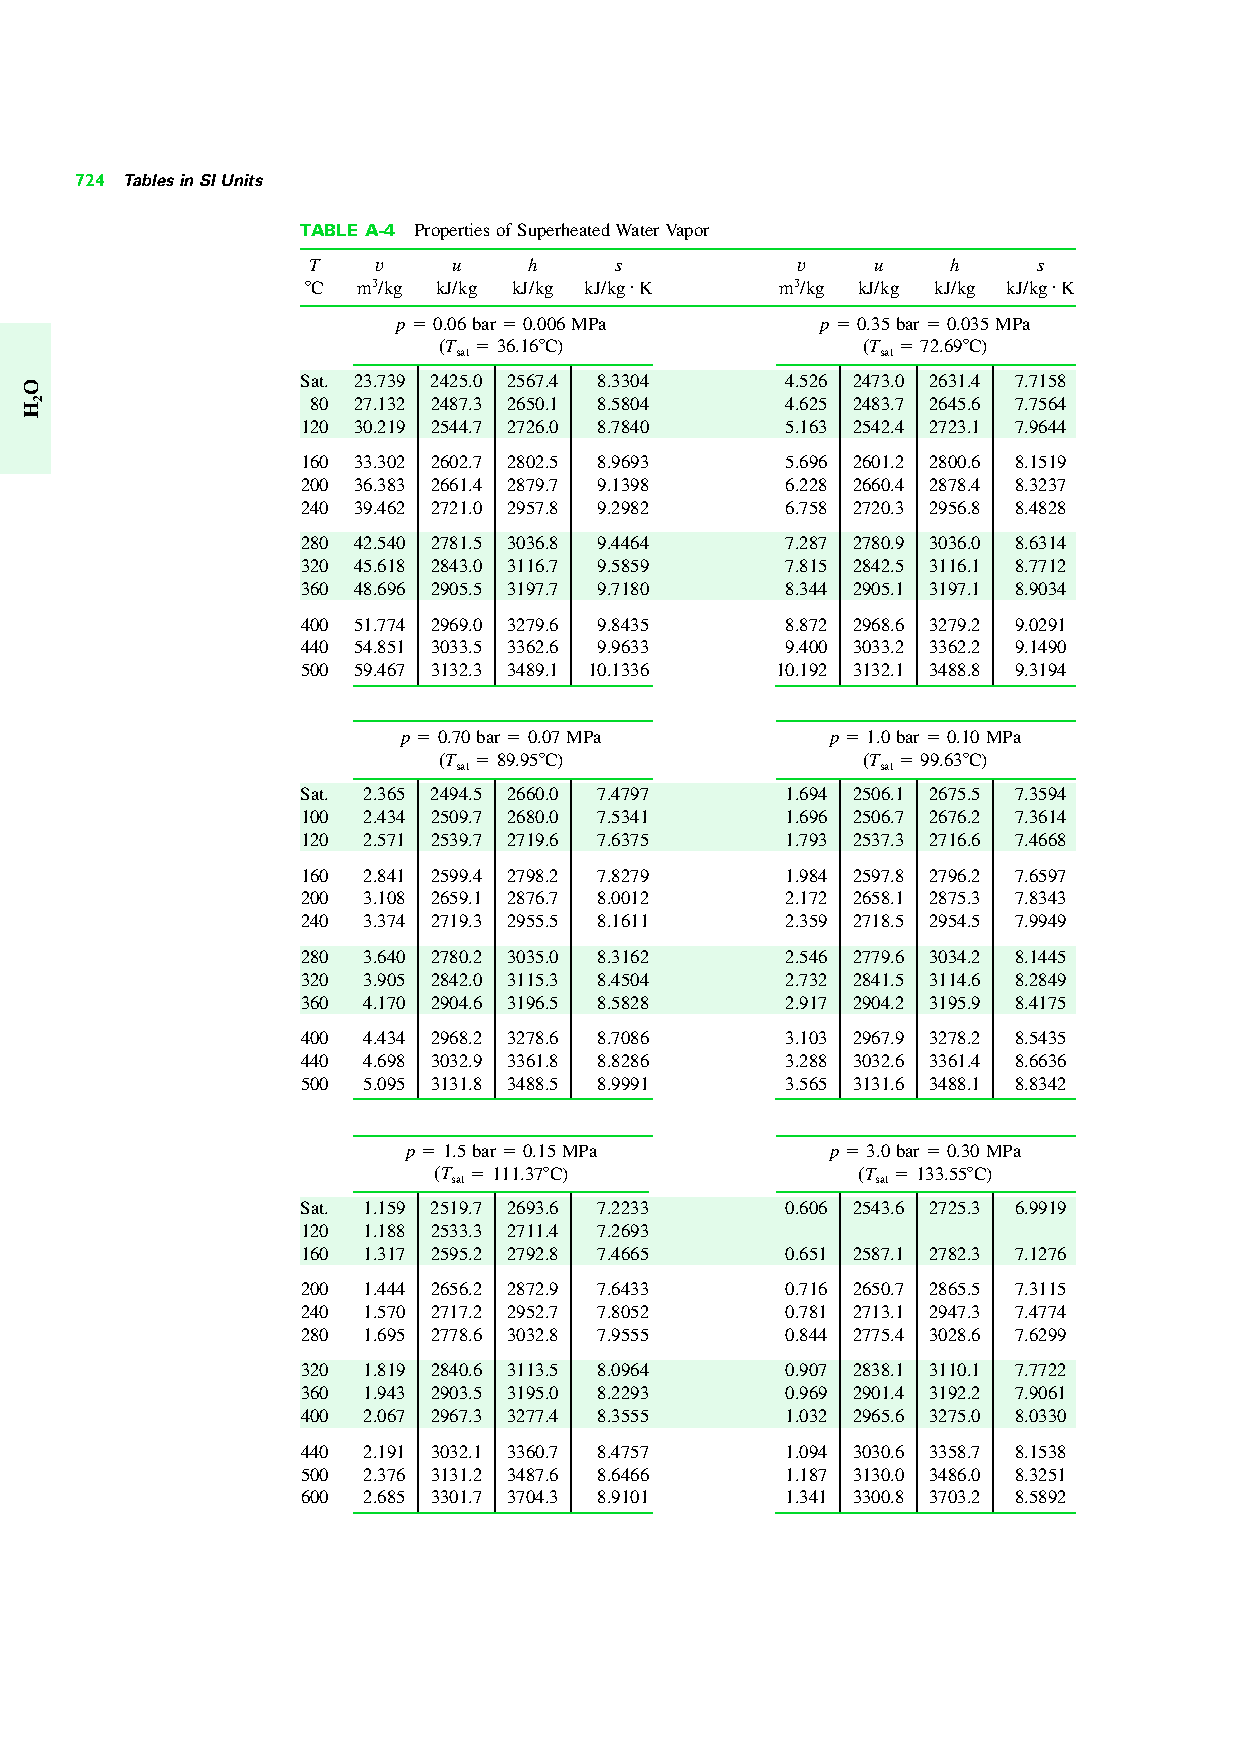
\includegraphics[width=9.5cm,height=8.5cm,clip]{./../Pics/Water_SuperheatedTable} 
   \end{figure}
   \end{center}
\end{frame}


%%%
%%% Slide
%%%
\begin{frame}
  \frametitle{Another option: (a) Saturated and (b) Superheated Tables with (c) \red{Linear Interpolation}}
\noindent
\begin{enumerate}\scriptsize
\item <1-> {\bf \textcolor{red}{Example:}} At $P=1.50\;$ bar, the saturated steam has the following thermodynamic properties,
%\tiny 
\begin{center}
%\begin{table}[h]
\visible<2->{\begin{tabular}{c c|c c c|c c|c c} 
%\hline\hline
$P$ & $T$ & $h_{f}$ &  $h_{fg}$ & $h_{g}$ & $s_{f}$ &  $s_{g}$ & $v_{f}$ & $v_{g}$ \\ 
\hline
1.50 & 111.4 & 467.11 & 2226.5 & 2693.6 & 1.4336 & 7.2233 & 0.0010528 & 1.159 \\
%\hline
\end{tabular}
where: [$P$] = bar, [$T$] = $^{o}$C, [$h$]= $\frac{kJ}{kg}$, [$s$]=$\frac{kJ}{kg.K}$, [$v$]=$\frac{m^{3}}{kg}$.}
\end{center}

\item <3-> But the properties of superheated steam at the same pressure will depend on the temperature $\Rightarrow$ \textcolor{red}{see superheated steam table}. Thus at 1.50 bar $\left(\text{with }T_{\text{sat}}=111.4^{\circ}\text{C}\right)$:
  \visible<3->{\begin{center}\begin{tabular}{ c | c c c}
      $T$    & $v$    & $h$     &    $s$     \\
\hline
      111.4  & 1.159  & 2693.6  &  7.2233    \\
      120.0  & 1.188  & 2711.4  &  7.2693    \\
      160.0  & 1.317  & 2792.8  &  7.4665    \\
      200.0  & 1.444  & 2872.9  &  7.6433    \\
      240.0  & 1.570  & 2952.7  &  7.8052    \\ 
     $\vdots$& $\vdots$&$\vdots$&$\vdots$ \\
  \end{tabular}
  \end{center}
}
\item <4-> Some of the problems in this course involves extracting values from the thermodynamic tables;
\item <5-> And although the tables are very extensive (for most of the materials), sometimes we need values that can not be directly found on them;
\item <6-> In this case, we just operate a {\bf linear interpolation} between neighbour fields;
\item <7-> For example, \underline{water-steam at 1.50 bar and 212$^{o}$C};
\item <8-> At this pressure, the {\bf saturation temperature} is 111.3$^{o}$C, therefore we know that the fluid (water/steam) is at \textcolor{red}{superheated state};

\end{enumerate}

\end{frame}

%%%
%%% Slide
%%%
\begin{frame}
  \frametitle{Another option: (a) Saturated and (b) Superheated Tables with (c) \red{Linear Interpolation}}
\noindent
\begin{enumerate}\setcounter{enumi}{7}\scriptsize
\item <1-> Thus at 1.50 bar and 212$^{\circ}$C, enthalpy and entropy of superheated steam are within the following interval:
  \visible<1->{\begin{center}\begin{tabular}{ c | c c c}
      $T$    & $v$    & $h$     &    $s$     \\
      \textcolor{red}{200.0}  & 1.444  & \textcolor{red}{2872.9}  &  7.6433    \\
      \textcolor{red}{240.0}  & 1.570  & \textcolor{red}{2952.7}  &  7.8052    \\ 
  \end{tabular}
  \end{center}
}
\item<2-> The enthalpy at 212$^{o}$C can be calculated as,
\visible<3->{\begin{tabular}{ l l }
\scriptsize $\Delta T=T_{2}-T_{1}=240-200^{o}$C   & \scriptsize $\longleftrightarrow$  $\Delta h=h_{2}-h_{1}=2952.7-2872.9=79.8\frac{kJ}{kg}$ \\
\scriptsize $\Delta T^{\star} = T_{2} - T^{\star}= 240 - 212^{\circ}$C & \scriptsize $\longleftrightarrow$  $\Delta h^{\star}= h_{2} - h^{\star}= 2952.7 - h^{\star}$\\    
\end{tabular}}
\item <4-> $\Delta h^{\star}=55.86\frac{kJ}{kg}$ 
\item <4-> Thus $\Delta h^{\star}= h_{2}-h^{\star} \longrightarrow h\left(T=212^{\circ}C\right)=h^{\star}=2896.84\frac{kJ}{kg}$.
\item<5-> Similarly for entropy: $s\left(T=212^{\circ}C\right)=s^{\star}=7.6919\frac{kJ}{kg.K}$.
\end{enumerate}

\end{frame}


%%%
%%% Slide
%%%

\begin{frame}
  \frametitle{Third Option: PVT Software and Websites}
\noindent
\begin{itemize}
   \item<1-> \href{http://www.weatherford.com/doc/wft183650}{PVTflex$^{TM}$};
   \item<1-> \href{http://www.kbcat.com/infochem-software/flow-assurance-software-multiflash/pvt-simulation}{Multiflash$^{TM}$};
   \item<1-> \href{https://www.honeywellprocess.com/en-US/explore/products/advanced-applications/unisim/Pages/default.aspx}{UniSim – Software for Process Design and Simulation};
   \item<1-> \href{http://webbook.nist.gov/chemistry/fluid/}{NIST Website}
   \item<1-> etc.
\end{itemize}

\end{frame}

\end{comment}

%%%
%%% SECTION
%%%
\section{Laws of Thermodynamics}


%%%
%%% SUBSECTION
%%%
\subsection{Zeroth Law of Thermodynamics}

%%%
%%% Slide
%%%
\begin{frame}
 \frametitle{Zeroth Law of Thermodynamics (Thermal Equilibrium)}

 \begin{columns}
  \begin{column}[r]{0.4\linewidth}
   \begin{block}{R.H. Fowler (1931)}
   \textcolor{blue}{$\lq$Two bodies are in equilibrium if both have the same temperature reading even if they are not in contact.'}
   \end{block}
    $ T_{j} = T_{i}
    \begin{cases}
     \forall_{i}, \forall{j} \\
     i \neq j
    \end{cases}$
  \end{column}
  
  \begin{column}[c]{0.6\linewidth}
\scriptsize \textcolor{blue}{Two bodies reaching thermal equilibrium after being brought into contact in an isolated enclosure.}
   \begin{figure}%
    \begin{center}
     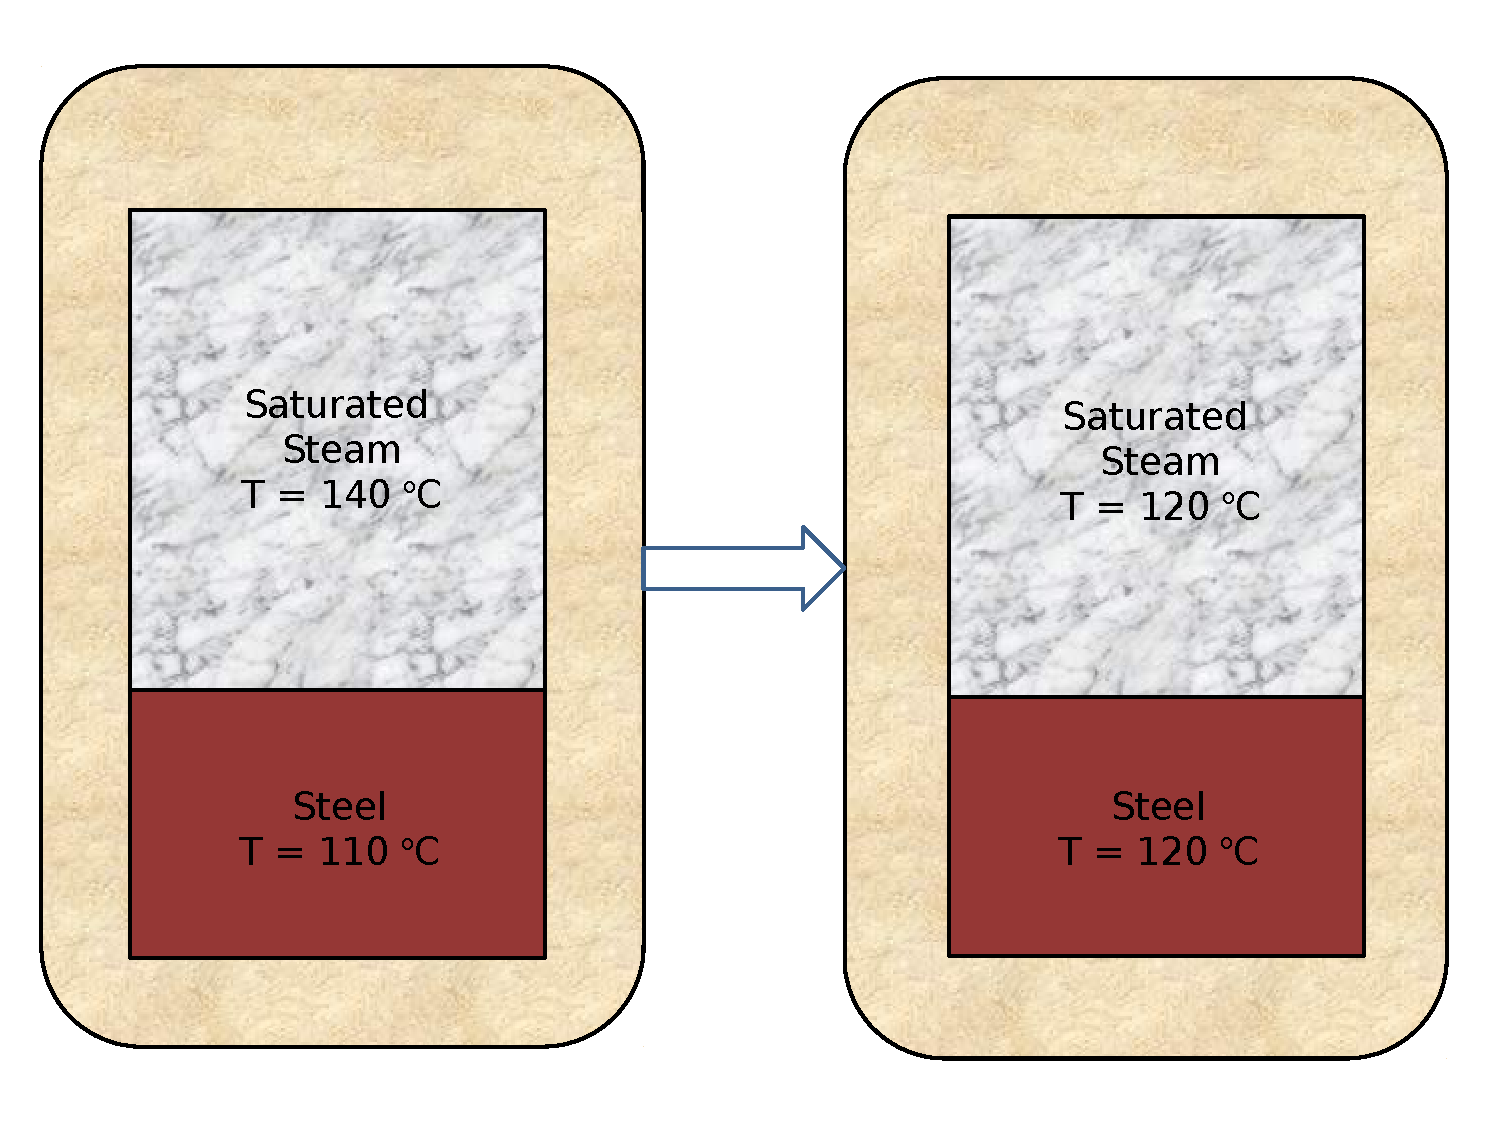
\includegraphics[width=\columnwidth,clip]{./../Pics/zeroth_law}\\
      \scriptsize \textcolor{blue}{$t = 0 \hspace{3.cm} \text{equilibrium state}$}
    \end{center}
   \end{figure}
  \end{column}
 \end{columns}

\end{frame}


%%%
%%% SUBSECTION
%%%
\subsection{First Law of Thermodynamics}

%%%
%%% Slide
%%%
\begin{frame}
 \frametitle{First Law of Thermodynamics (Conservation of Work)}
 %\scriptsize

 \begin{block}{R. Clausius and J.P. Joule (1850)}
  \textcolor{blue}{$\lq$For all adiabatic processes between two specified states of a closed system, the net work done is the same regardless of the nature of the closed system and the details of the process.}
  \begin{center}
   \textcolor{red}{or}
  \end{center}
  \textcolor{blue}{$\lq$Although energy assumes many forms, the total quantity of energy is constant, and when energy disappears in one form it appears simultaneously in other forms.}'
 \end{block}


 \begin{itemize}
  \item<2-> It states that energy can neither be created, nor can it be destroyed. This means that the total amount of energy in the universe always remains conserved;
  \item<3-> Energy can be changed from one form to another. There are many different forms of energy, some of which may be more useful than others for a particular process;
 \end{itemize}

\normalsize
\end{frame}

%%%
%%% Slide
%%%
\begin{frame}
 \frametitle{First Law of Thermodynamics (Conservation of Energy)}
 %\scriptsize
   \begin{enumerate}
      \item<1-> A system (e.g., a fluid) can possess energy:
        \begin{itemize}
          \item<1-> as a result of its macroscopic position (potential) or movement (kinetic);
          \item<1-> or as a result of microscopic/molecular motion $\rightarrow$ {\it internal energy}.
        \end{itemize}
\visible<2->{
      \begin{block}{Conservation of Energy}
        \begin{center}
          \textcolor{blue}{$\Delta E$ (system) + $\Delta E$ (surroundings) = 0}
        \end{center}
      \end{block}}

      \item<3-> Heat and work represent energy in transit across boundaries -- system and surroundings.

   \end{enumerate}
\normalsize
\end{frame}



%%%
%%% Slide
%%%
\begin{frame}\label{Slide1}
 \frametitle{First Law of Thermodynamics (Conservation of Energy in Closed Systems)}
 %\scriptsize
   \begin{enumerate} 
      \item<1-> Closed systems $\longrightarrow$ $dm = 0$
         \visible<1->{
         \begin{center}
           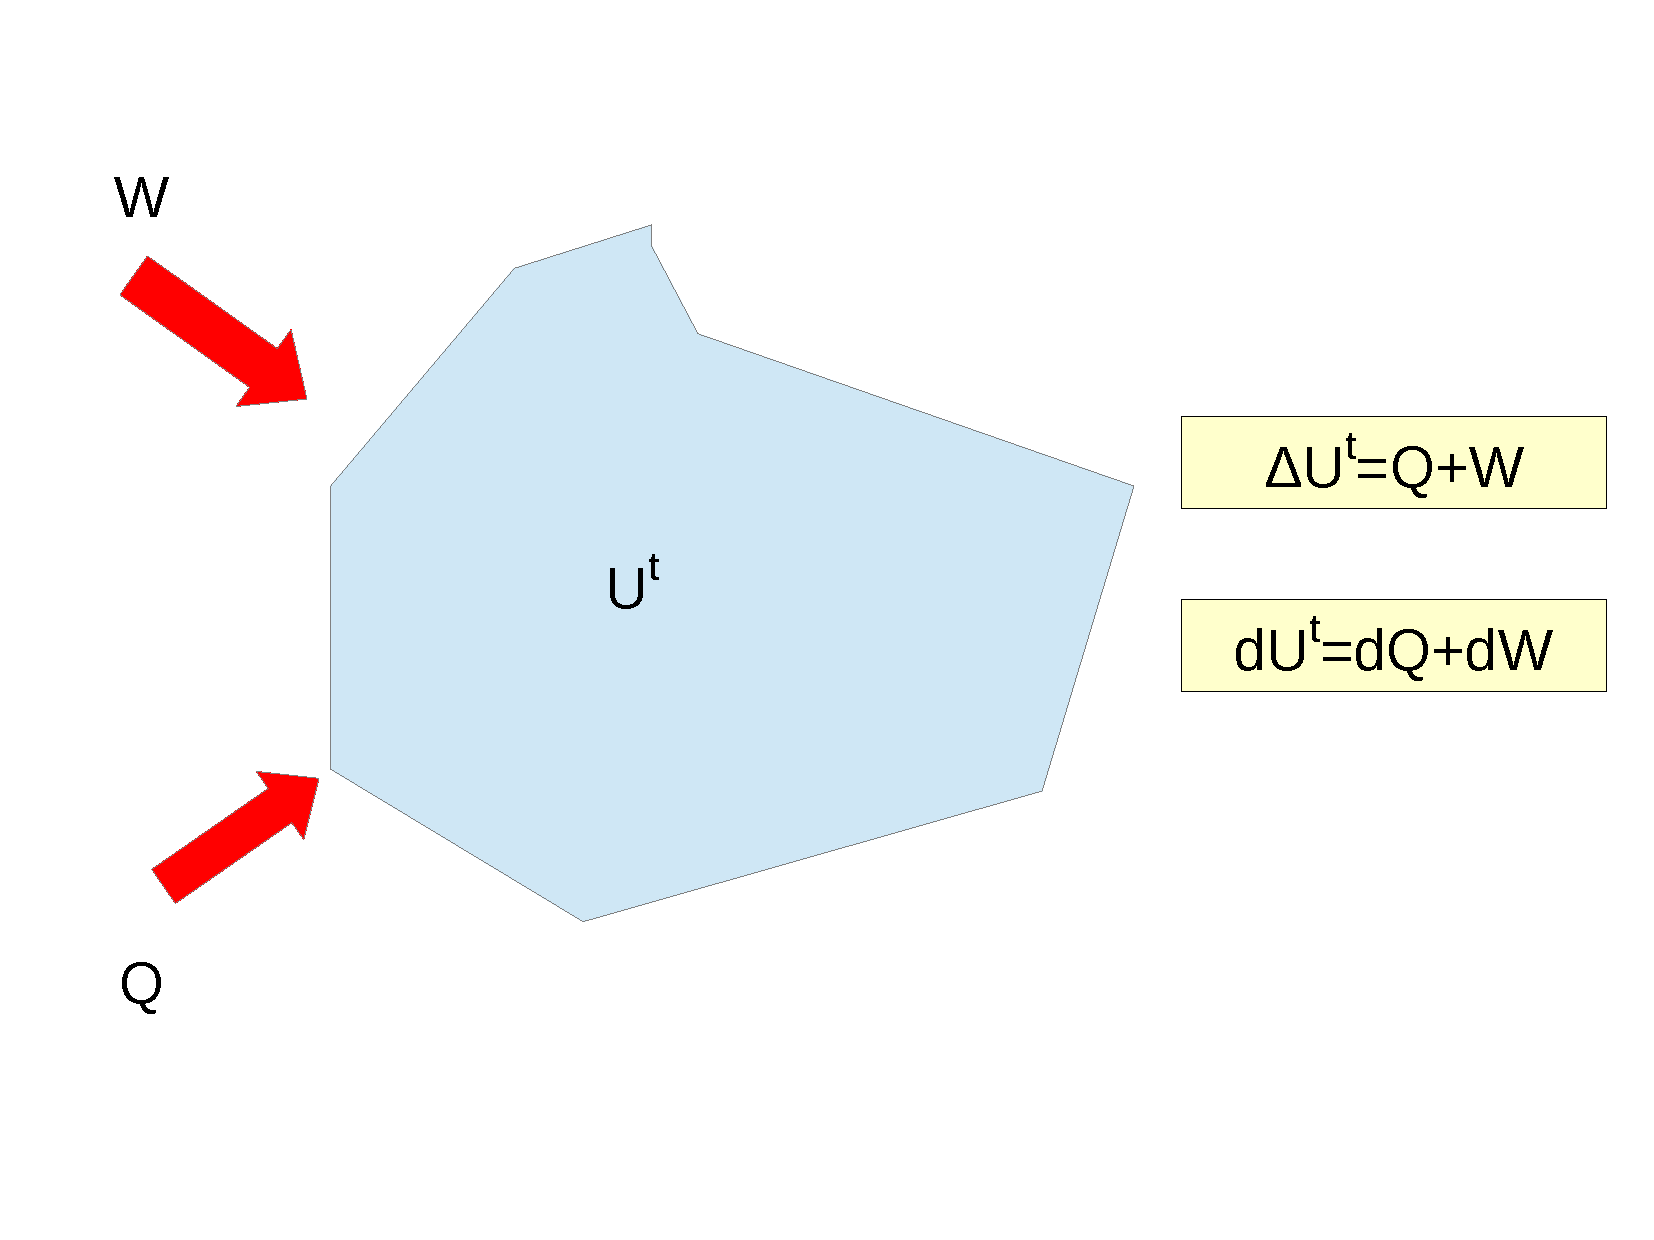
\includegraphics[width=6.cm,clip]{./../Pics/Energy_ClosedSystems}
         \end{center}}
      \item<2-> \href{http://www.iupac.org/}{IUPAC} (International Union of Pure and Applied Chemistry) sign convention:
         \begin{itemize}
            \item<2-> Heat ($Q$) and work ($W$)  always refer to the system;
            \item<2-> Energy transfer to the system has always a \textcolor{blue}{positive sign}.
         \end{itemize}
   \end{enumerate}
\normalsize
\end{frame}


%%%
%%% Slide
%%%
\begin{frame}
 \frametitle{Representations of the First Law -- Cycle}

 \begin{block}{}During any cycle, the cyclic integral of heat added to a system is proportional to the cyclic integral of work done by the system.\end{block}

 The mathematical representation of the first law is
 \begin{equation}
  \displaystyle\oint \delta Q = \displaystyle\oint \delta W
  \label{Module00:first_law}
 \end{equation}
 with {\it [Q] = J} and {\it [W] = J}. The symbol $\displaystyle\oint$ represents {\it line integral}, see more details in \blue{\it Appendices$\_$Thermodynamics.pdf} document in {\it MyA}.

\end{frame}

%%%
%%% Slide
%%%
\begin{frame}
 \frametitle{Representations of the First Law -- Cycle}
 %\scriptsize
 \begin{columns}
  \begin{column}[l]{0.5\linewidth}
   \begin{itemize}
    \item <1-> \textcolor{blue}{Power cycle}: systems (e.g., rhs) that deliver a net work transfer of energy to their surroundings during each cycle;
    \item <2-> $W_{cycle} = Q_{in} - Q_{out}$ with $Q_{in} > Q_{out}$ for a power cycle;
    \item <3-> The energy supplied by heat transfer to a system on a power cycle is normally derived from combustion (also from nuclear fission or solar radiation). The energy $Q_{out}$ is generally discharged to the surrounding atmosphere or a nearby body of water;
   \end{itemize}
  \end{column}
   
  \begin{column}[l]{0.5\linewidth}
   \begin{figure}%
    \begin{center}
     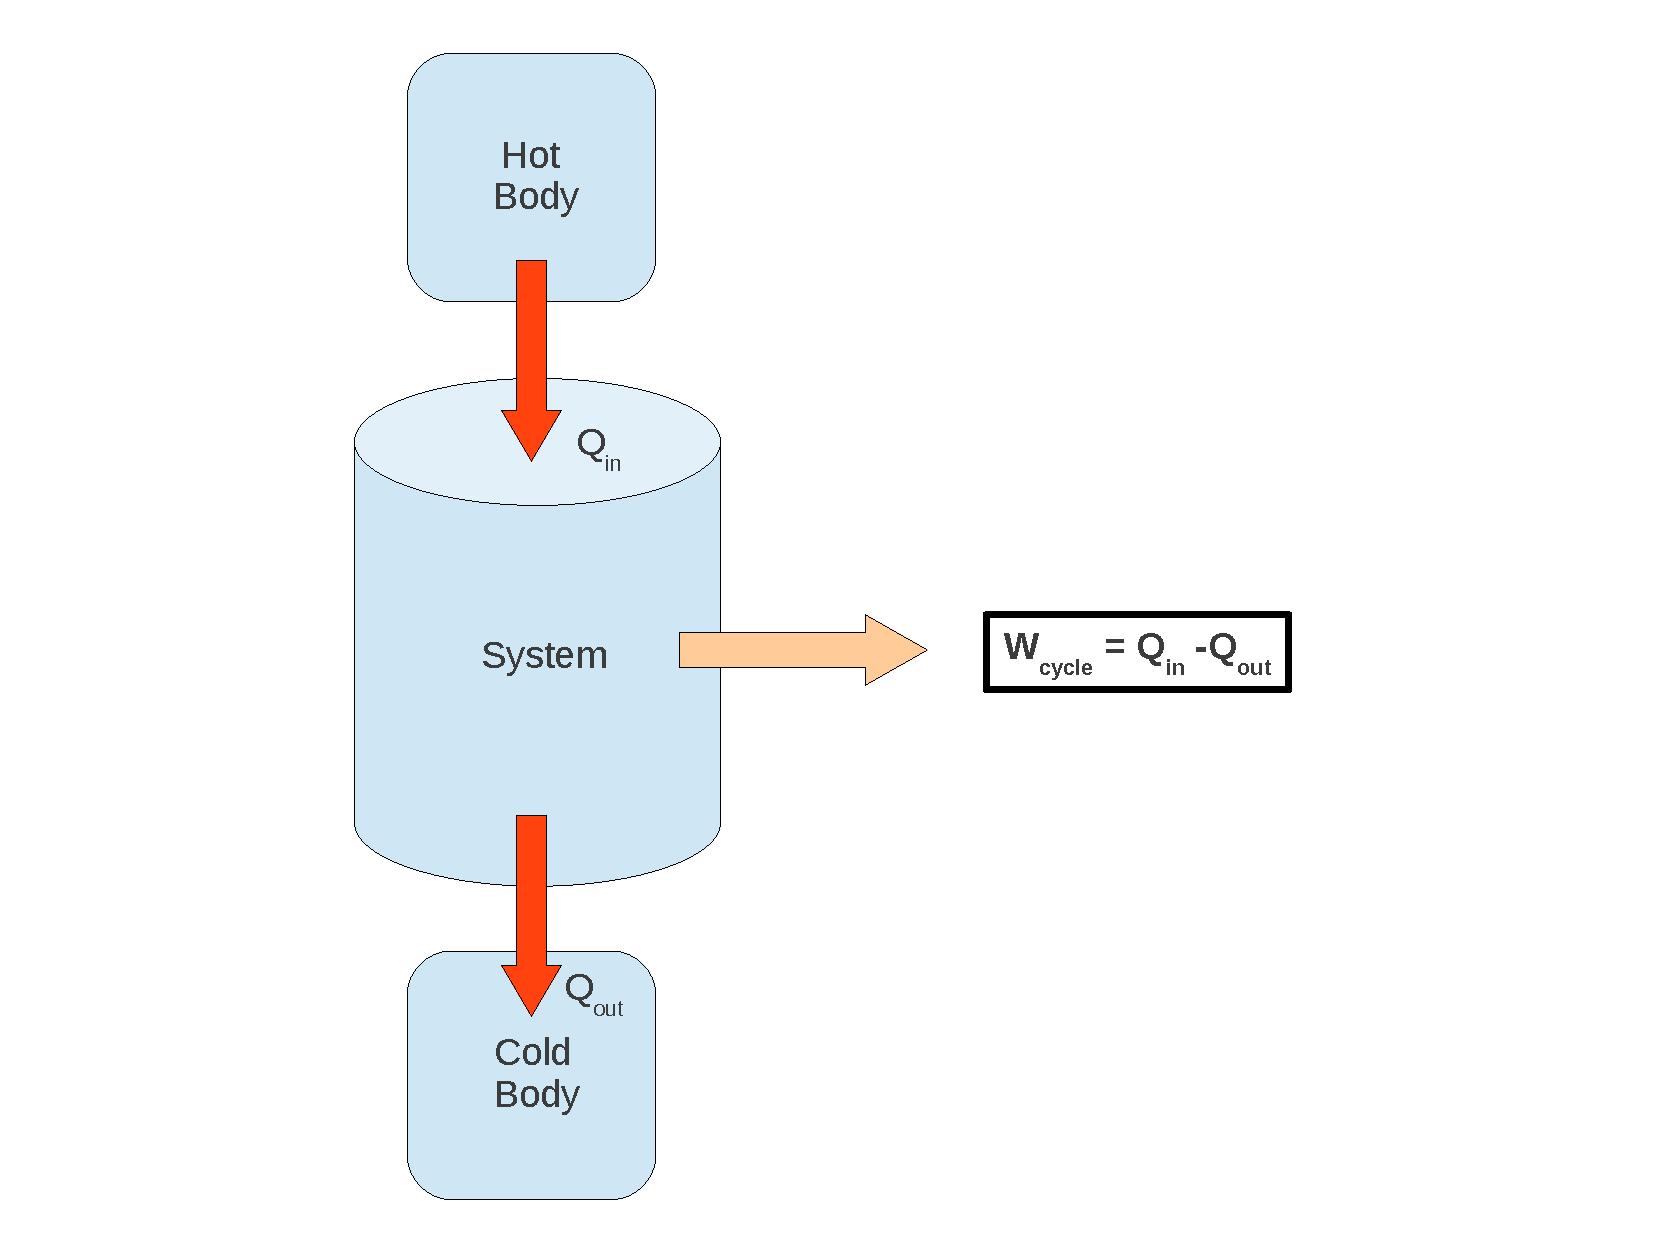
\includegraphics[width=8.cm,clip]{./../Pics/FirstLaw_Cycle_01}
    \end{center}
   \end{figure}    
  \end{column}
 \end{columns}
 \normalsize
\end{frame}


%%%
%%% Slide
%%%
\begin{frame}
 \frametitle{Representations of the First Law -- Cycle}
 %\scriptsize
 \begin{columns}
  \begin{column}[l]{0.5\linewidth}
   \begin{itemize}
    \item <1-> \textcolor{blue}{Thermal efficiency}: $\eta =\displaystyle\frac{W_{cycle}}{Q_{in}} = \displaystyle\frac{Q_{in} - Q_{out}}{Q_{in}} = 1 - \displaystyle\frac{Q_{out}}{Q_{in}} < 1$;
    \item <2-> For reversible power cycles the ratio of heat transfer, $Q_{cold}/Q_{hot}$ depends only on the reservoir temperatures: $Q_{cold}/Q_{hot} = T_{cold}/T_{hot}$;
    \item <3-> Thus the thermal efficiency of a reversible power cycle while operating between thermal reservoirs at temperatures $T_{hot}$ and $T_{cold}$ is expressed as,\\
          $\eta_{max} = 1 - \displaystyle\frac{T_{cold}}{T_{hot}}$
   \end{itemize}
  \end{column}
   
  \begin{column}[l]{0.5\linewidth}
   \begin{itemize}
    \item <4-> This is the \textcolor{blue}{Carnot efficiency} and it is the maximum efficiency any power cycle can have while operating between the 2 reservoirs.
   \end{itemize}\vspace{-.5cm}
   \begin{figure}%
    \begin{center}
     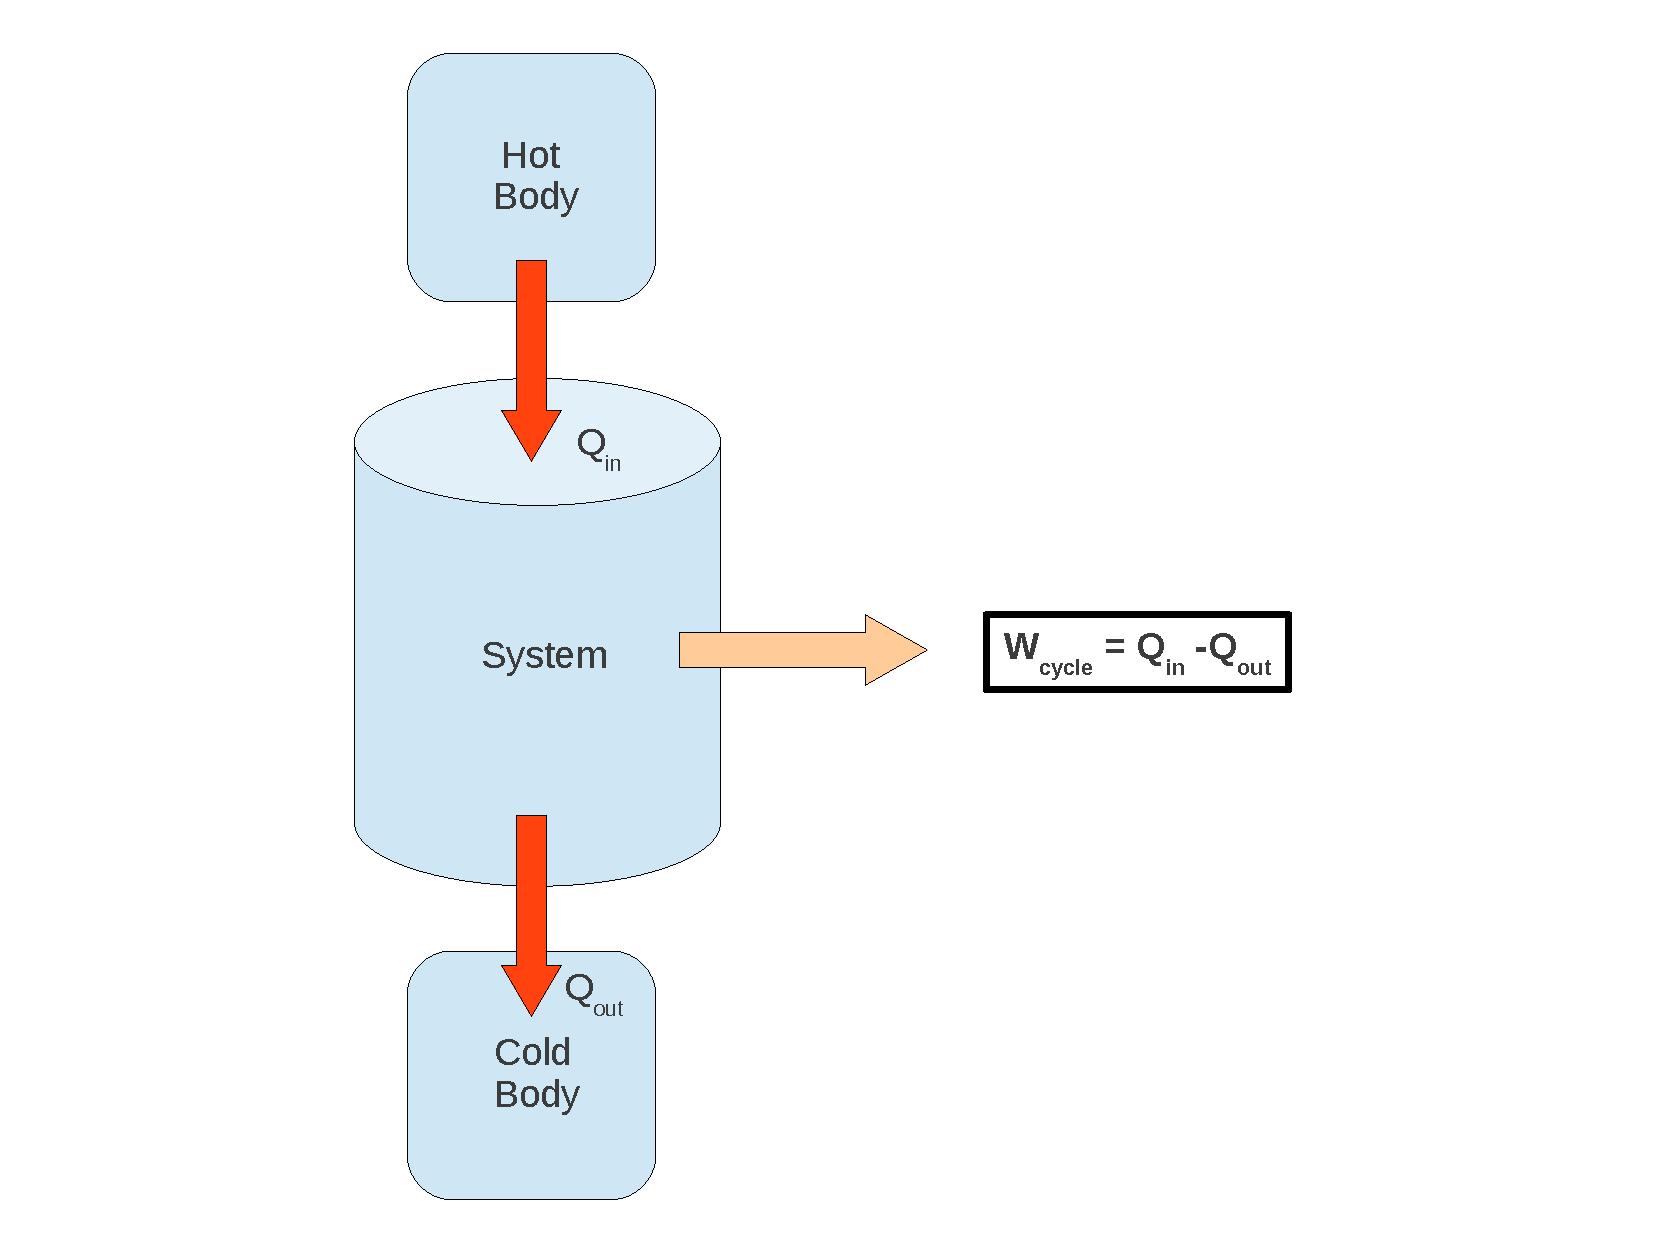
\includegraphics[width=8.cm,clip]{./../Pics/FirstLaw_Cycle_01}
    \end{center}
   \end{figure}    
  \end{column}
 \end{columns}
 \normalsize
\end{frame}


%%%
%%% Slide
%%%
\begin{frame}
 \frametitle{Representations of the First Law -- Cycle}
 \begin{columns}
  \begin{column}[l]{0.5\linewidth}
   \begin{itemize}%\scriptsize
      \item <1-> \textcolor{blue}{Refrigeration} Cycles (rhs) aim to cool a refrigerated body or to maintain the temperature of a body bellow that of the surroundings;
      \item <2-> Q$_{in}$ is associated with the heat energy transferred into the system from the cold body, whereas Q$_{out}$ is the energy discharged via heat transfer from the system to the hot body. The work required for the cycle is,
             \visible<2->{\begin{displaymath}
                 W_{cycle} = Q_{out} - Q_{in}
             \end{displaymath}}\vspace{-0.5cm}
      \item <3-> Coefficient of Performance: 
             \visible<3->{\begin{displaymath}
                 \beta = \frc{Q_{in}}{W_{cycle}} = \frc{Q_{in}}{Q_{out} - Q_{in}}
             \end{displaymath}}
    \end{itemize}
  \end{column}
   
  \begin{column}[c]{0.5\linewidth}
     \begin{itemize}[(c)]%\scriptsize
      \item <4-> E.g., in a fridge: cavity contents $\xrightarrow{Q_{in}}$ refrigerant fluid $\left(T_{fluid} < T_{cavity}\right)$ $\xrightarrow{Q_{out}}$ surrounding air; 
     \end{itemize}
\vspace{-.8cm}
   \begin{figure}%
     \hbox{\hspace{-.5cm}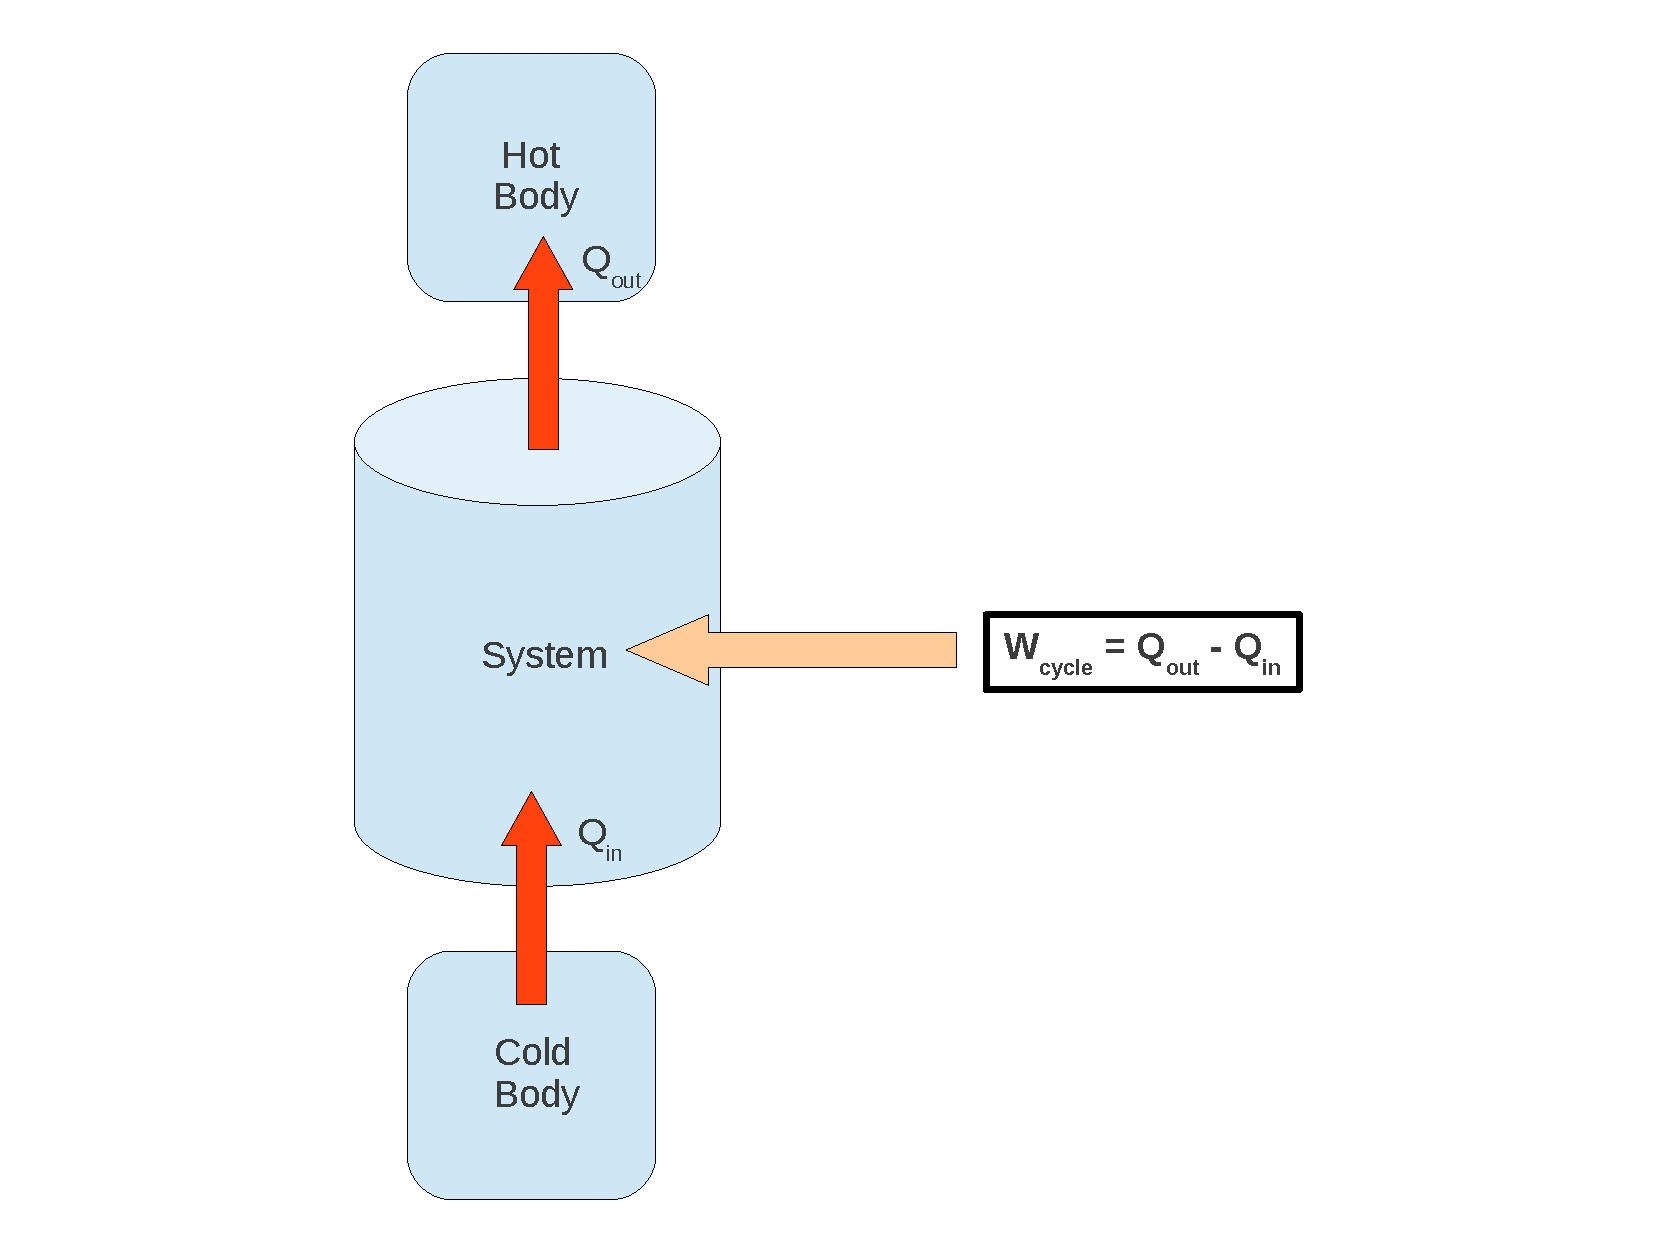
\includegraphics[width=8.cm,clip]{./../Pics/FirstLaw_Cycle_02}}
   \end{figure}    
  \end{column}
 \end{columns}
 \normalsize
\end{frame}

\begin{comment}
%%%
%%% Slide
%%%
\begin{frame}
 \frametitle{Representations of the First Law -- Cycle}
 \begin{columns}
  \begin{column}[l]{0.5\linewidth}
   \begin{itemize}
    \item <1-> \textcolor{blue}{Heat pump cycle}:
     \begin{enumerate}[(a)]
      \item <2-> Objective: to maintain a heated space at a high temperature by absorbing heat from a low-temperature source (e.g., well water or cold outside air), and supplying this heat to the high-temperature medium (e.g., house);
      \item <3-> Coefficient of Performance: $\gamma = \displaystyle\frac{Q_{out}}{W_{cycle}} = \displaystyle\frac{Q_{out}}{Q_{out} - Q_{in}} = \beta + 1 \geq 1$;
      \item <4-> E.g., a fridge in a window (with the door open to cold outside environment): outside surrounding air $\xrightarrow{Q_{in}}$ refrigerant fluid $\left(T_{fluid} < T_{cavity}\right)$ $\xrightarrow{Q_{out}}$ inside the house; 
     \end{enumerate}
   \end{itemize}
  \end{column}
   
  \begin{column}[c]{0.5\linewidth}
   \begin{figure}%
    \begin{center}
     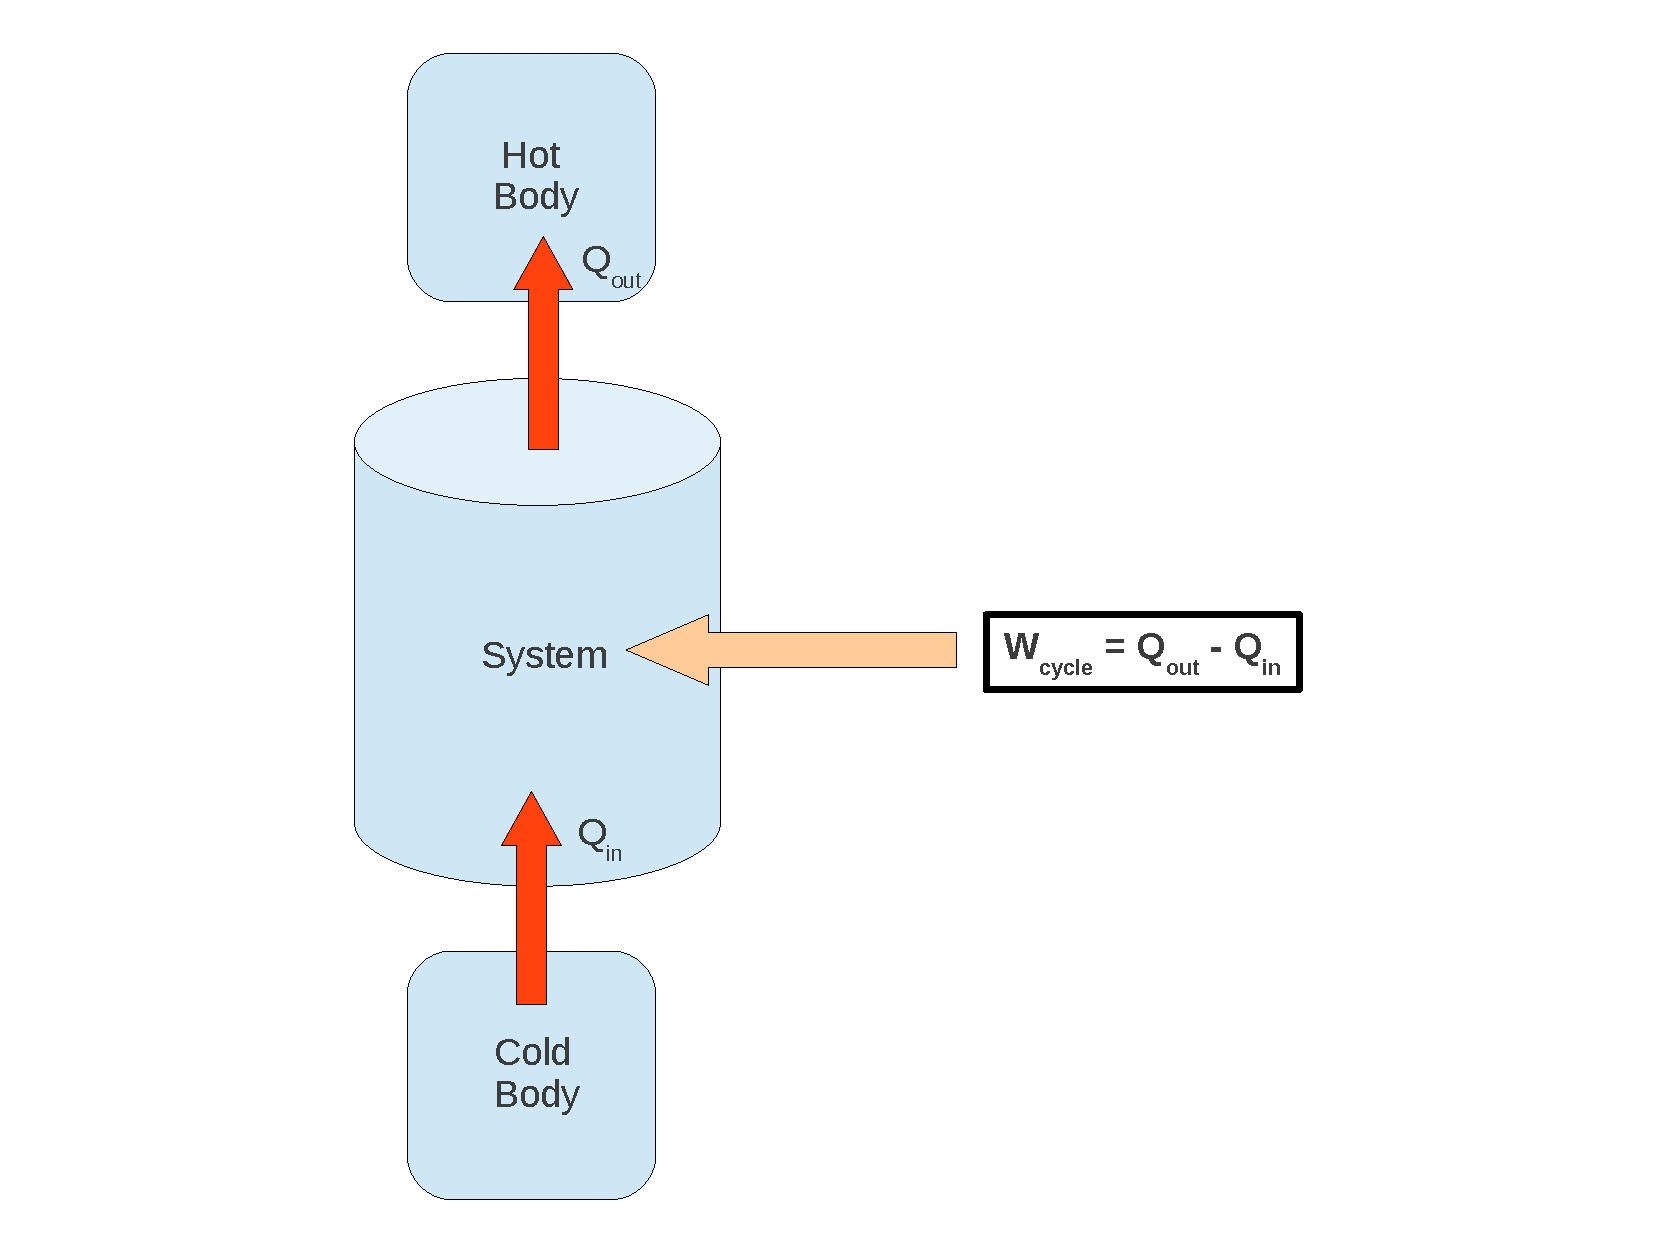
\includegraphics[width=8.cm,clip]{./../Pics/FirstLaw_Cycle_02}
    \end{center}
   \end{figure}    
  \end{column}
 \end{columns}
 \normalsize
\end{frame}


\end{comment}
%%%
%%% Slide
%%%
\begin{frame}
 \frametitle{Example 1: Thermodynamic Cycle}
   \textcolor{blue}{{\it {\bf Example:} A gas undergoes a thermodynamic cycle consisting of three processes: 
   \begin{enumerate}[(a)]
    \item \textcolor{blue}{{\it 1-2}: compression with $PV$ = constant, from $P_{1}$ = 1 bar, V$_{1}$ = 1.6m$^{3}$ to V$_{2}$ = 0.2m$^{3}$, U$_{2}$ - U$_{1}$ = 0.0 J;}
    \item \textcolor{blue}{{\it 2-3}: constant pressure to V$_{3}$ = V$_{1}$;}
    \item \textcolor{blue}{{\it 3-1}: constant volume, U$_{1}$ - U$_{3}$ = -3549 kJ.}
   \end{enumerate}
   There are no significant changes in kinetic or potential energy. Determine the heat transfer and work for process 2–3 (in kJ). Is this a power cycle or a refrigeration cycle?}}

   Let's assume that the gas is a closed system and the only work done is due to volume change. In order to compute the work for process {\it 2-3} with constant pressure,\\
   %\begin{displaymath}
    $W_{2}^{3} = \int\limits_{V_{2}}^{V_{3}} P dV = P_{2}\left(V_{3}-V_{2}\right)$\\
   %\end{displaymath}
   Using the {\it PV} relation for process {\it 1-2} $\rightarrow$ $P_{2}=P_{1}V_{1}V_{2}^{-1}=8\text{ bar}$. Thus , with $V_{3}=V_{1}$,\\
   $W_{2}^{3} = ( 8 bar ) \left[ \left( 1.6m^{3}\right) - \left( 0.2m^{3}\right) \right]$\\
   $\;\;\;\;\;\; = 11.2 \;bar.m^{3} \left[\textcolor{blue}{\frac{10^{5}N.m^{-2}}{1\; bar}\frac{1\; J}{1\; N.m}\frac{1\; kJ}{10^{3}\; J}}\right]= \textcolor{red}{1120 kJ}$
 \normalsize
\end{frame}


%%%
%%% Slide
%%%
\begin{frame}
 \frametitle{Example 1: Thermodynamic Cycle}

   The energy balance for process {\it 2-3} reduces to $Q_{2}^{3}=\left(U_{3}-U_{2}\right)+W_{2}^{3}$. \\
   Remember that in a cycle, $\left(\Delta U\right)_{\text{cycle}}=0$, therefore:\\
   $\left(U_{2}-U_{1}\right) + \left(U_{3}-U_{2}\right) + \left(U_{1}-U_{3}\right)=0$\\
   $\left(U_{3}-U_{2}\right) = - \left(U_{1}-U_{3}\right) = 3549 kJ$\\
   For process {\it 2-3}: $Q_{2}^{3}= 3549 + 1120 = \textcolor{red}{4669 kJ}$\\
\medskip

   For process {\it 1-2}: $\Delta U = 0$, \\
   $Q_{1}^{2} = W_{1}^{2} = \int_{V_{1}}^{V_{2}}P dV = P_{1}V_{1}\ln\left(V_{2}/V_{1}\right) $\\
   $\;\;\;\;\;=\textcolor{red}{-332.7 kJ}$\\
\medskip

   And for process {\it 3-1}: $W_{3}^{1}=0$ and $Q_{3}^{1}=U_{1}-U_{3}=\textcolor{red}{-3549 kJ}$. The cycle can then be calculated as,
   $W_{\text{cycle}}=W_{1}^{2}+W_{2}^{3}+W_{3}^{1} = -332.7 + 1120 + 0 = 787.3 kJ$\\

\medskip
   Since \textcolor{red}{$W_{\text{cycle}}>0$}, the cycle is a \textcolor{red}{power cycle}.
 \normalsize
\end{frame}

%%%
%%% Slide
%%%
\begin{frame}
 \frametitle{Representations of the First Law -- Process}

   Let's consider the set of paths from state 1 to 2:
   \begin{itemize}
    \item Cycle I: 1 to 2 on Path A followed by 2 to 1 on Path B;
    \item Cycle II: 1 to 2 on Path A followed by 2 to 1 on Path C;
   \end{itemize}

   \begin{figure}%
    \begin{center}
     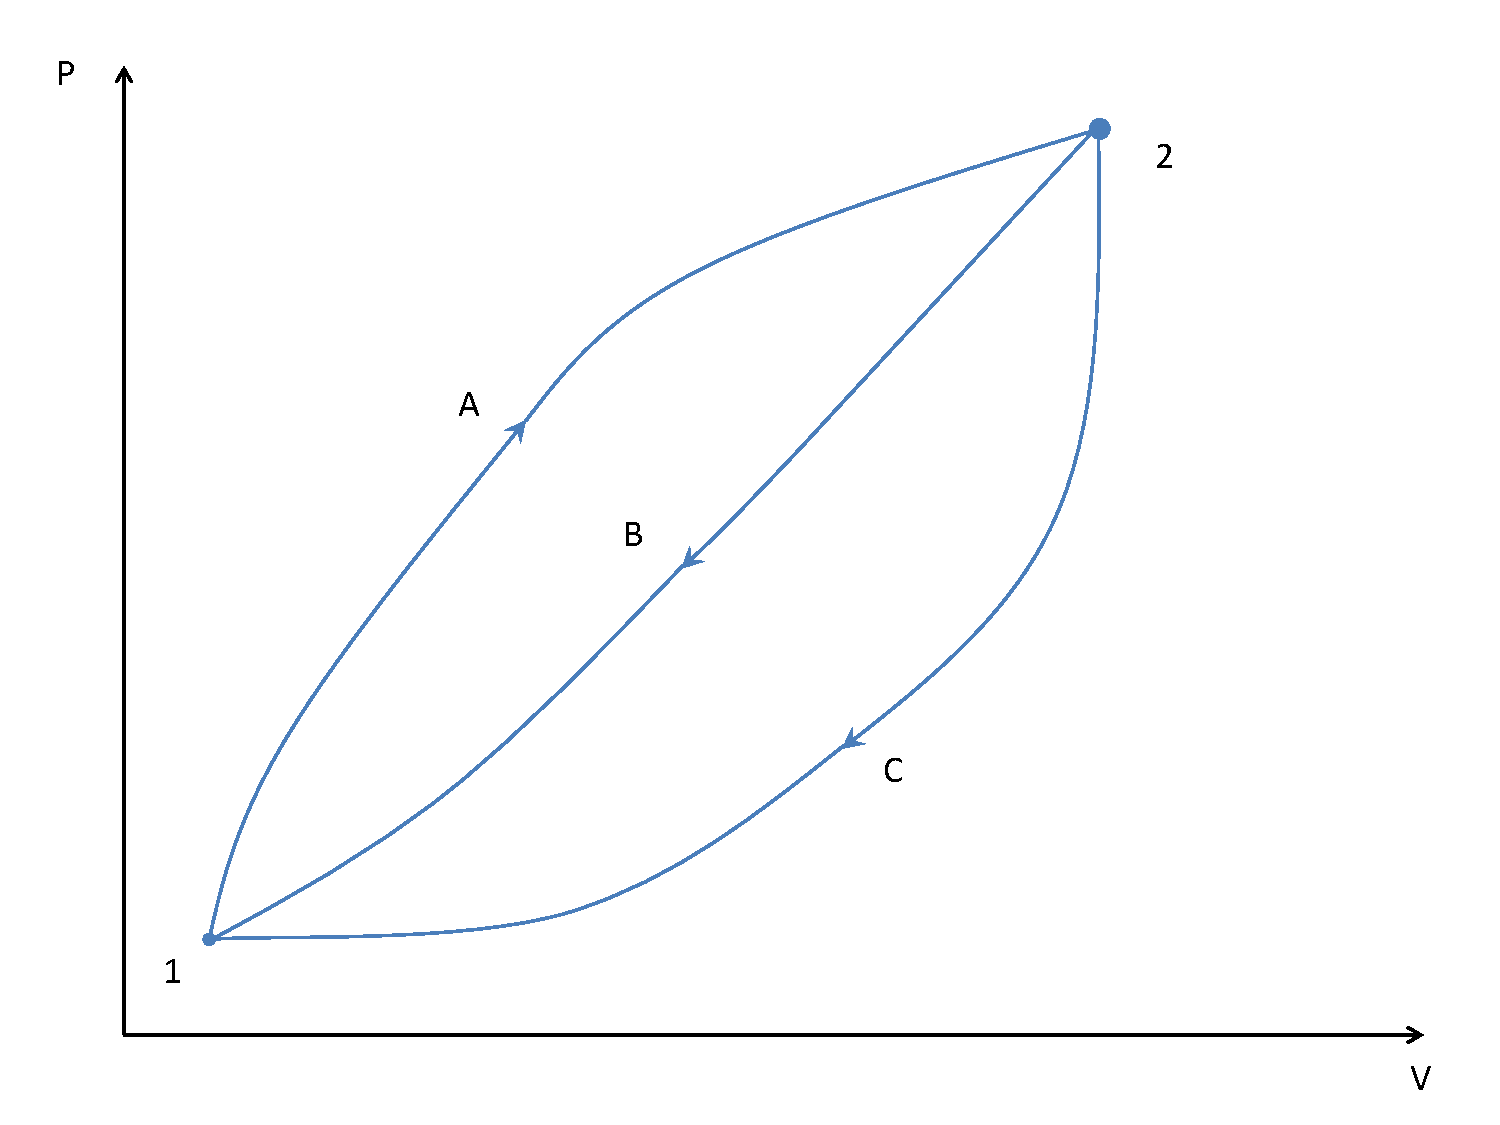
\includegraphics[width=7.5cm,clip]{./../Pics/first_law_process}
     %\caption{P-V diagram for various combinations of processes forming cyclic integrals.}
    \end{center}
   \end{figure}

\normalsize
\end{frame}


%%%
%%% Slide
%%%
\begin{frame}
 \frametitle{Representations of the First Law -- Process}
   \begin{itemize}
    \item <1-> These cycles can be mathematically represented using Eqn. \ref{Module00:first_law}:
   \begin{eqnarray}
    \text{Cycle I:}  \int\limits_{1}^{2}\delta Q_{A} + \int\limits_{2}^{1}\delta Q_{B} = \int\limits_{1}^{2}\delta W_{A} + \int\limits_{2}^{1}\delta W_{B}  \label{Module00:proc1a}\\
    \text{Cycle II:} \int\limits_{1}^{2}\delta Q_{A} + \int\limits_{2}^{1}\delta Q_{C} = \int\limits_{1}^{2}\delta W_{A} + \int\limits_{2}^{1}\delta W_{C}  \label{Module00:proc1b}
   \end{eqnarray}
   \item <2-> Subtracting Eqn. \ref{Module00:proc1b} from \ref{Module00:proc1a} and rearranging:
   \begin{equation}
    \int\limits_{2}^{1}\left(\delta Q- \delta W\right)_{B} = \int\limits_{2}^{1}\left(\delta Q- \delta W\right)_{C}\label{Module00:proc1c}
   \end{equation}
   \item <3-> B and C are arbitrary paths ; Eqn. \ref{Module00:proc1c} asserts that the integral of $\left(\delta Q -\delta W\right)\left.\right|_{2}^{1}$ is path-independent. Notice, however that both \textcolor{blue}{Q} and \textcolor{blue}{W} are path-dependent quantities. 
    \end{itemize}
\end{frame}



%%%
%%% Slide
%%%
\begin{frame}
 \frametitle{Representations of the First Law -- Process}

  \begin{itemize}
   \item <1-> Energy (as any property) depends only on the state and not on the path taken to arrive at the state. Defining the differential of U:\\
    $dU =\delta Q - \delta W$\\ 
   
   \item <2-> Integrating from 1 to 2:\\
    $\displaystyle\int\limits_{1}^{2}dU =\displaystyle\int\limits_{1}^{2}\delta Q - \displaystyle\int\limits_{1}^{2}\delta W$\\ 

   \item <3-> Leading to
   \begin{equation}
    U_{2} - U_{1} = Q_{1}^{2}- W_{1}^{2} \label{Module00:proc1d}
   \end{equation}

  \end{itemize}
\normalsize
\end{frame}



%%%
%%% Slide
%%%
\begin{frame}
 \frametitle{Representations of the First Law -- Process}
 \begin{block}{Another way to state the First Law} 
  For a system undergoing a process, the change in energy is equal to the \underline{heat added to the system} \red{and} the \underline{work done by the system}.
  \begin{displaymath}
     dU =\delta Q \pm \delta W 
  \end{displaymath}
 \end{block}
Note that the sign convention (Slide~\ref{Slide1}) should be used here, i.e., positive sign for energy (as heat and work) flowing into the system and negative sign for energy flowing out of the system. Thus,
  \begin{equation}
     dU =\delta Q - \delta W 
  \end{equation}
\end{frame}


%%%
%%% Slide
%%%
\begin{frame}
 \frametitle{Example 2: Conservation of Work}
 \scriptsize
 \begin{columns}
  \begin{column}[r]{0.5\linewidth}
   \begin{figure}%
    \begin{center}
     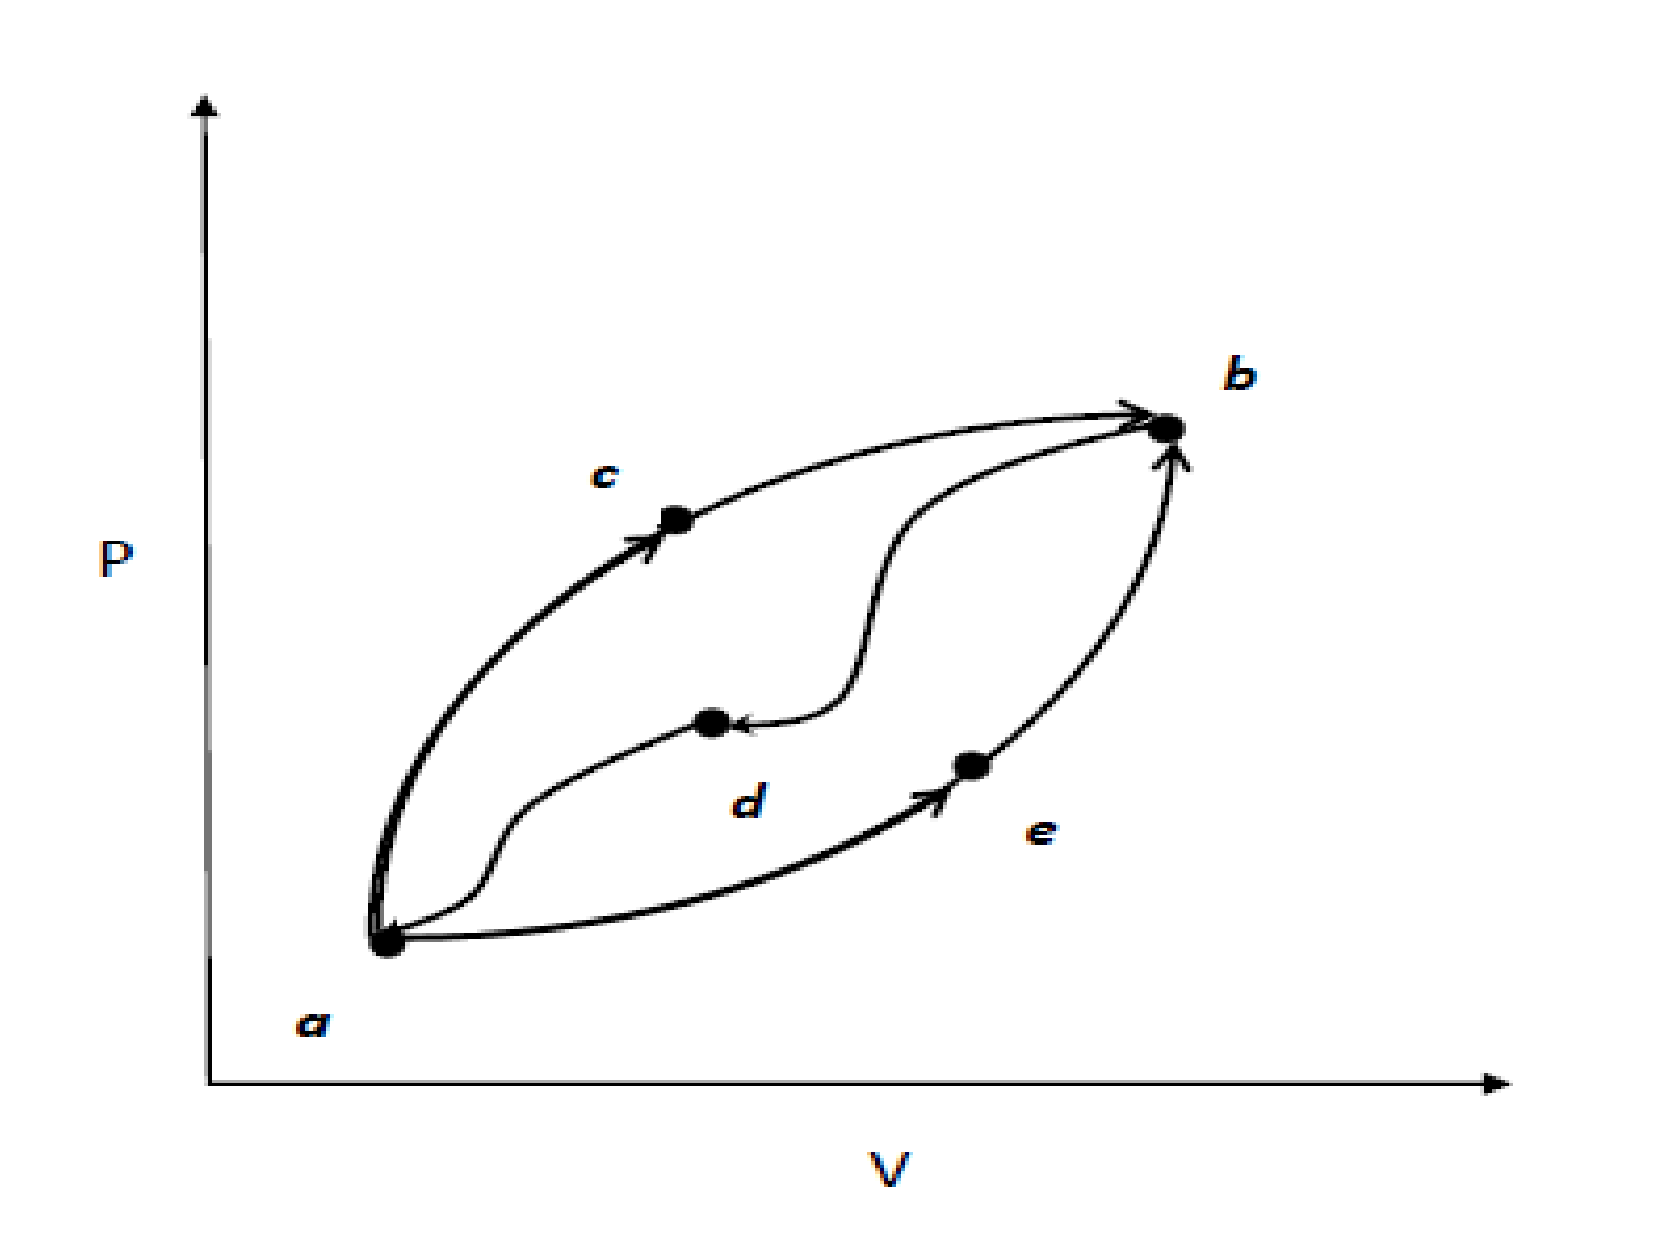
\includegraphics[width=\columnwidth,clip]{./../Pics/First_Law_1}
    \end{center}
   \end{figure}
   \visible<1->{When a system is taken from state \textcolor{blue}{a} to state \textcolor{blue}{b} along path \textcolor{blue}{acb}, 100 J of heat flows into the system and the system does 40 J of work.}
  \end{column}
  \begin{column}[r]{0.5\linewidth}
   \begin{enumerate}
    \item<2-> How much heat flows into the system along path \textcolor{blue}{aeb} if the work done by the system is 20 J?
       \begin{itemize}\scriptsize
         \item<3-> For path \textcolor{blue}{acb}:
           \begin{displaymath}
             \Delta U_{ab} = Q_{acb}-W_{acb} = 100 - 40 = 60 J
            \end{displaymath}
          \item<4-> For path \textcolor{blue}{aeb}:
            \begin{eqnarray}
              &&\Delta U_{ab} = Q_{aeb}-W_{aeb} = 60 J \nonumber \\
              &&\Delta U_{ab} = Q_{aeb}-20 \therefore Q_{aeb} = 80 J \nonumber
            \end{eqnarray}
       \end{itemize}

    \item<5-> The system returns from \textcolor{blue}{b} to \textcolor{blue}{a} along path \textcolor{blue}{bda}. If the \red{work done on the system} is 30 J, does the system absorb or liberate heat? How much? 
       \begin{itemize}\scriptsize
         \item<6-> For path \textcolor{blue}{bda}:
           \begin{eqnarray}
            &&\visible<7->{\Delta U_{ba} = -60 J = Q_{bda}-W_{bda}} \nonumber \\
            &&\visible<8->{\Delta U_{ba} = Q_{bda} \red{+ 30}} \visible<9->{\therefore Q_{bda} = -90 J} \nonumber
           \end{eqnarray}
         \item<10-> Thus, 90J of heat is \bf{released from the systems to the surroundings}.
       \end{itemize}
   \end{enumerate}
  \end{column}
 \end{columns}
\normalsize
\end{frame}


%%%
%%% Slides
%%%
\begin{frame}
 \frametitle{Reversible Processes}
   \begin{itemize}
    \item When an object at temperature $T=T\left(t_{0}\right)$ is left in a room in contact with ambient air, it is intuitive that the object will cool down at time $t_{1}$ and the air will warm up until the temperature of the body and the surrounding air are the same;
    \item From the First Law, we know that the {\it decrease in the internal energy of the body is equal to the increase in the internal energy of the surrounding air};
    \item The body cools down spontaneously and we can predict the {\it direction} of the process as it moves towards an equilibrium state, but; 
   \end{itemize}
    \begin{figure}%
     \begin{center}
      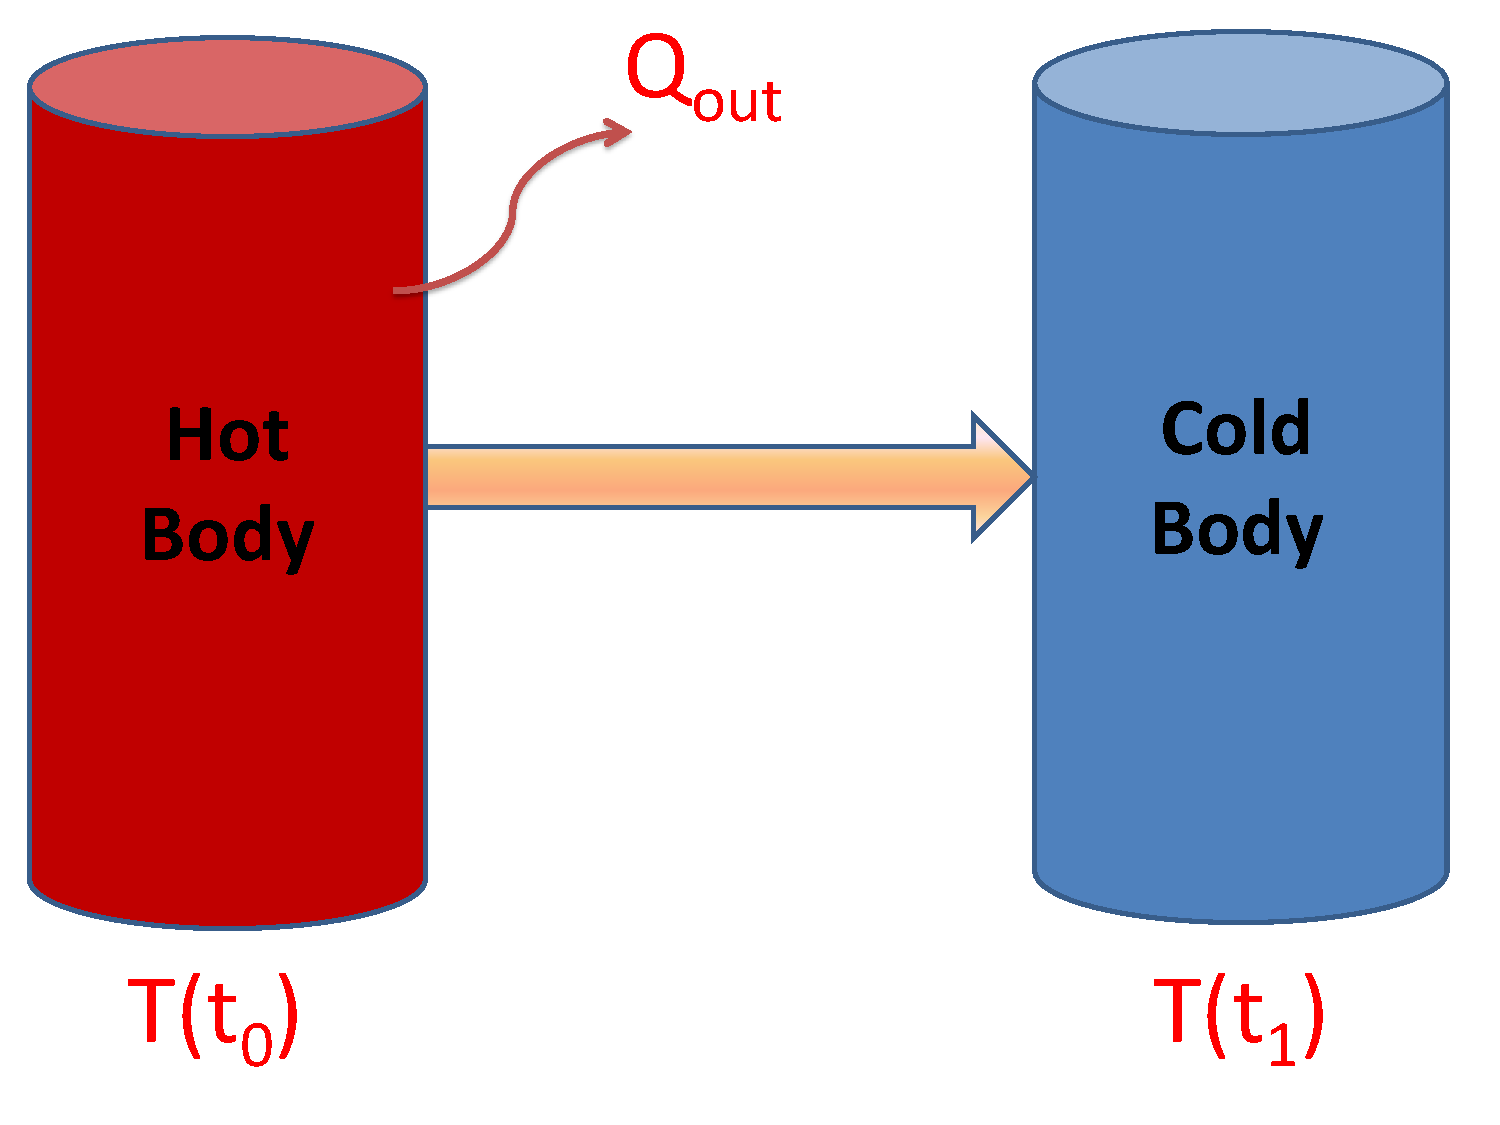
\includegraphics[width=5.5cm,clip]{./../Pics/HotColdCoffee}
     \end{center}
    \end{figure}
 \normalsize
\end{frame}


%%%
%%% Slides
%%%
\begin{frame}
 \frametitle{Reversible Processes}
   \begin{itemize}
    \item The initial state $\left(\text{i.e., }T_{0}\right)$ can be restored {\it but not spontaneously} $\Longrightarrow$  The reverse processes do not violate the First Law, and yet they {\it do not occur spontaneously};
    \item Another law is needed to help understand and predict which processes will occur spontaneously.
   \end{itemize}
    \begin{figure}%
     \begin{center}
      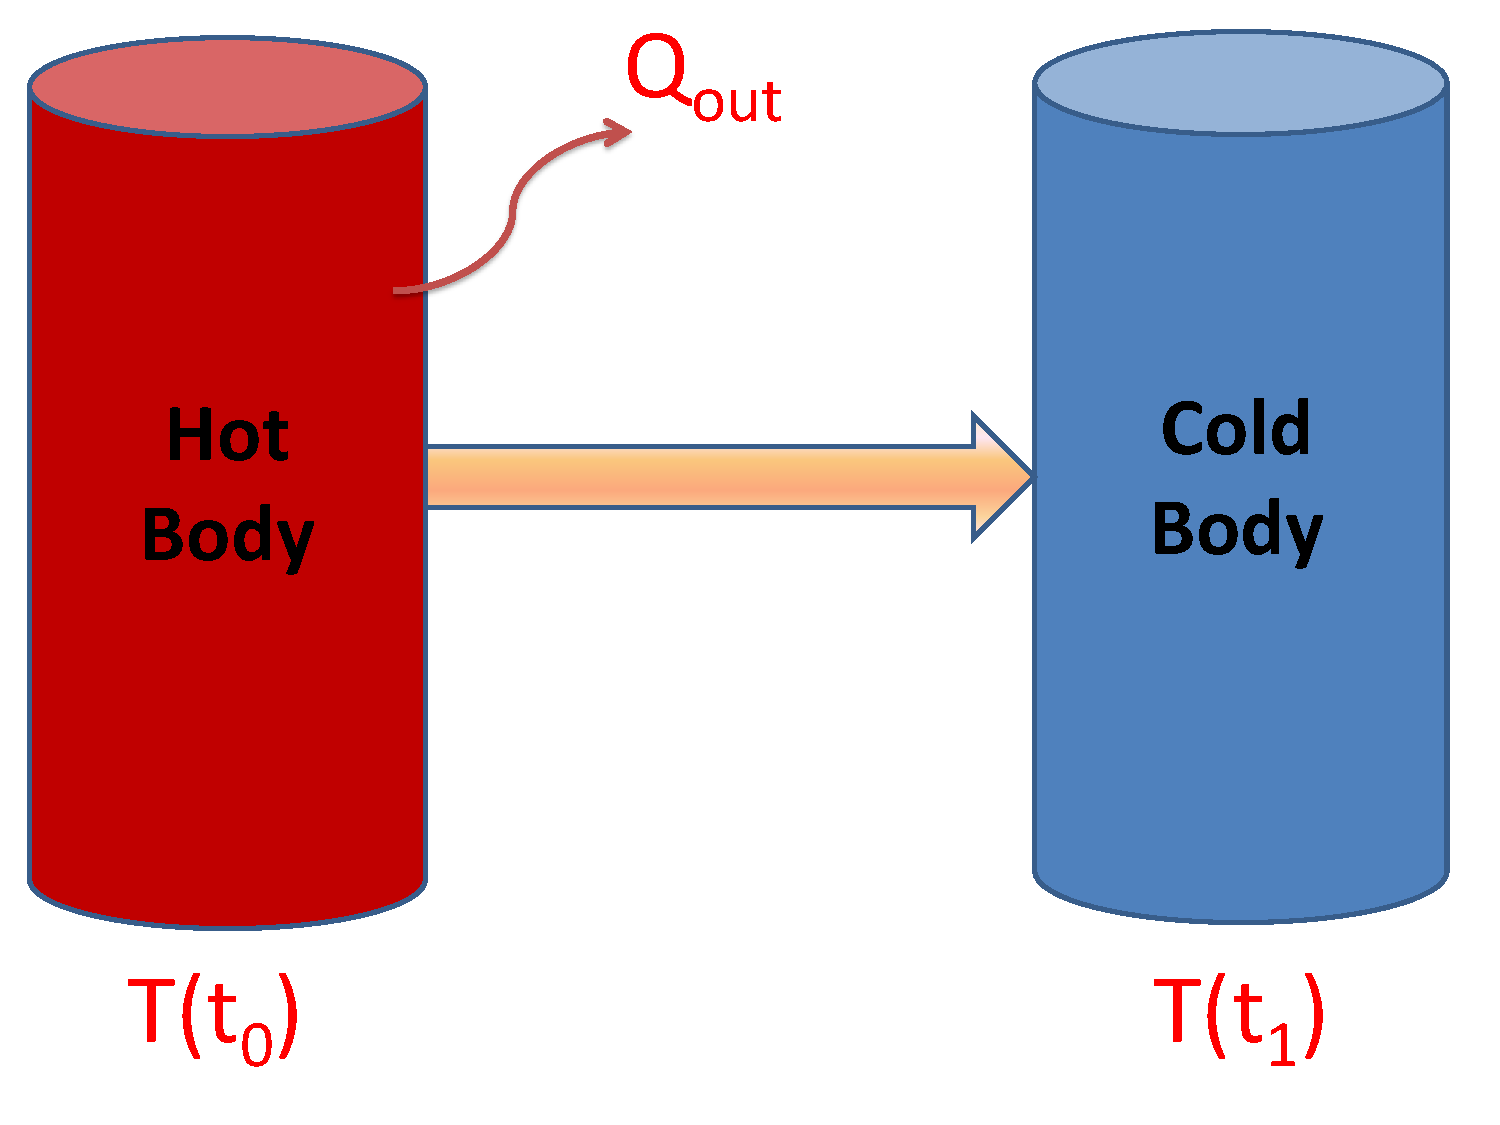
\includegraphics[width=5.5cm,clip]{./../Pics/HotColdCoffee}
     \end{center}
    \end{figure}
 \normalsize
\end{frame}


%%%
%%% Slides
%%%
\begin{frame}
 \frametitle{Reversible Processes}
 \begin{itemize}
  \item <2-> \textcolor{blue}{Reversible process:} A process in which it is possible to return both the system and surroundings to their original states;
  \item <3-> \textcolor{blue}{Irreversible process:} A process in which it is impossible to return both the system and surroundings to their original states.
 \end{itemize}

\end{frame}

%%%
%%% Slides
%%%
\begin{frame}
 \frametitle{Isochoric and Isobaric Processes}
     \visible<1->{\begin{block}{Energy conservation in a closed system:}
       $d U^{t}=d Q + d W$ \hspace{2cm} $d W = -P dV^{t}$ \hspace{2cm} $d U^{t}=d Q -P d V^{t}$
    \end{block}}

    \visible<2->{\begin{block}{Constant volume process (isochoric):}
       $-P d V^{t} =0$ \hspace{3cm} $d U^{t} = d Q$ \hspace{3cm} $\Delta U^{t}= Q $
    \end{block}}

    \visible<3->{\begin{block}{Constant pressure process (isobaric):}
       $d Q = d U^{t} + d\left(P V^{t}\right)= d\left(U^{t}+PV^{t}\right)$ \hspace{3cm} $H = U + PV$
    \end{block}}
 
 \normalsize
\end{frame}


%%%
%%% Slides
%%%
\begin{frame}
 \frametitle{Heat Capacity}
     \begin{itemize}
        \item<1-> General definition:
          \visible<1->{\begin{displaymath}
            C = \frac{dQ}{dT}
          \end{displaymath}}
        \item<2-> At \textcolor{blue}{constant volume}
             \visible<2->{\begin{displaymath}
                C_{V} = \left(\frac{\partial U}{\partial T}\right)_{V} \Longleftrightarrow  Q = n\Delta U = n\int\limits_{T_{1}}^{T_{2}} C_{V} dT
             \end{displaymath}}
        \item<3-> At \textcolor{blue}{constant pressure}
             \visible<2->{\begin{displaymath}
                C_{P} = \left(\frac{\partial H}{\partial T}\right)_{P} \Longleftrightarrow  Q = n\Delta H = n\int\limits_{T_{1}}^{T_{2}} C_{P} dT
             \end{displaymath}}
     \end{itemize}
 
 \normalsize
\end{frame}


%%%
%%% Slides
%%%
\begin{frame}
 \frametitle{Open Systems}
     \begin{itemize}
        \item<1-> Control volume and flow rates:
         \visible<1->{
         \begin{center}
           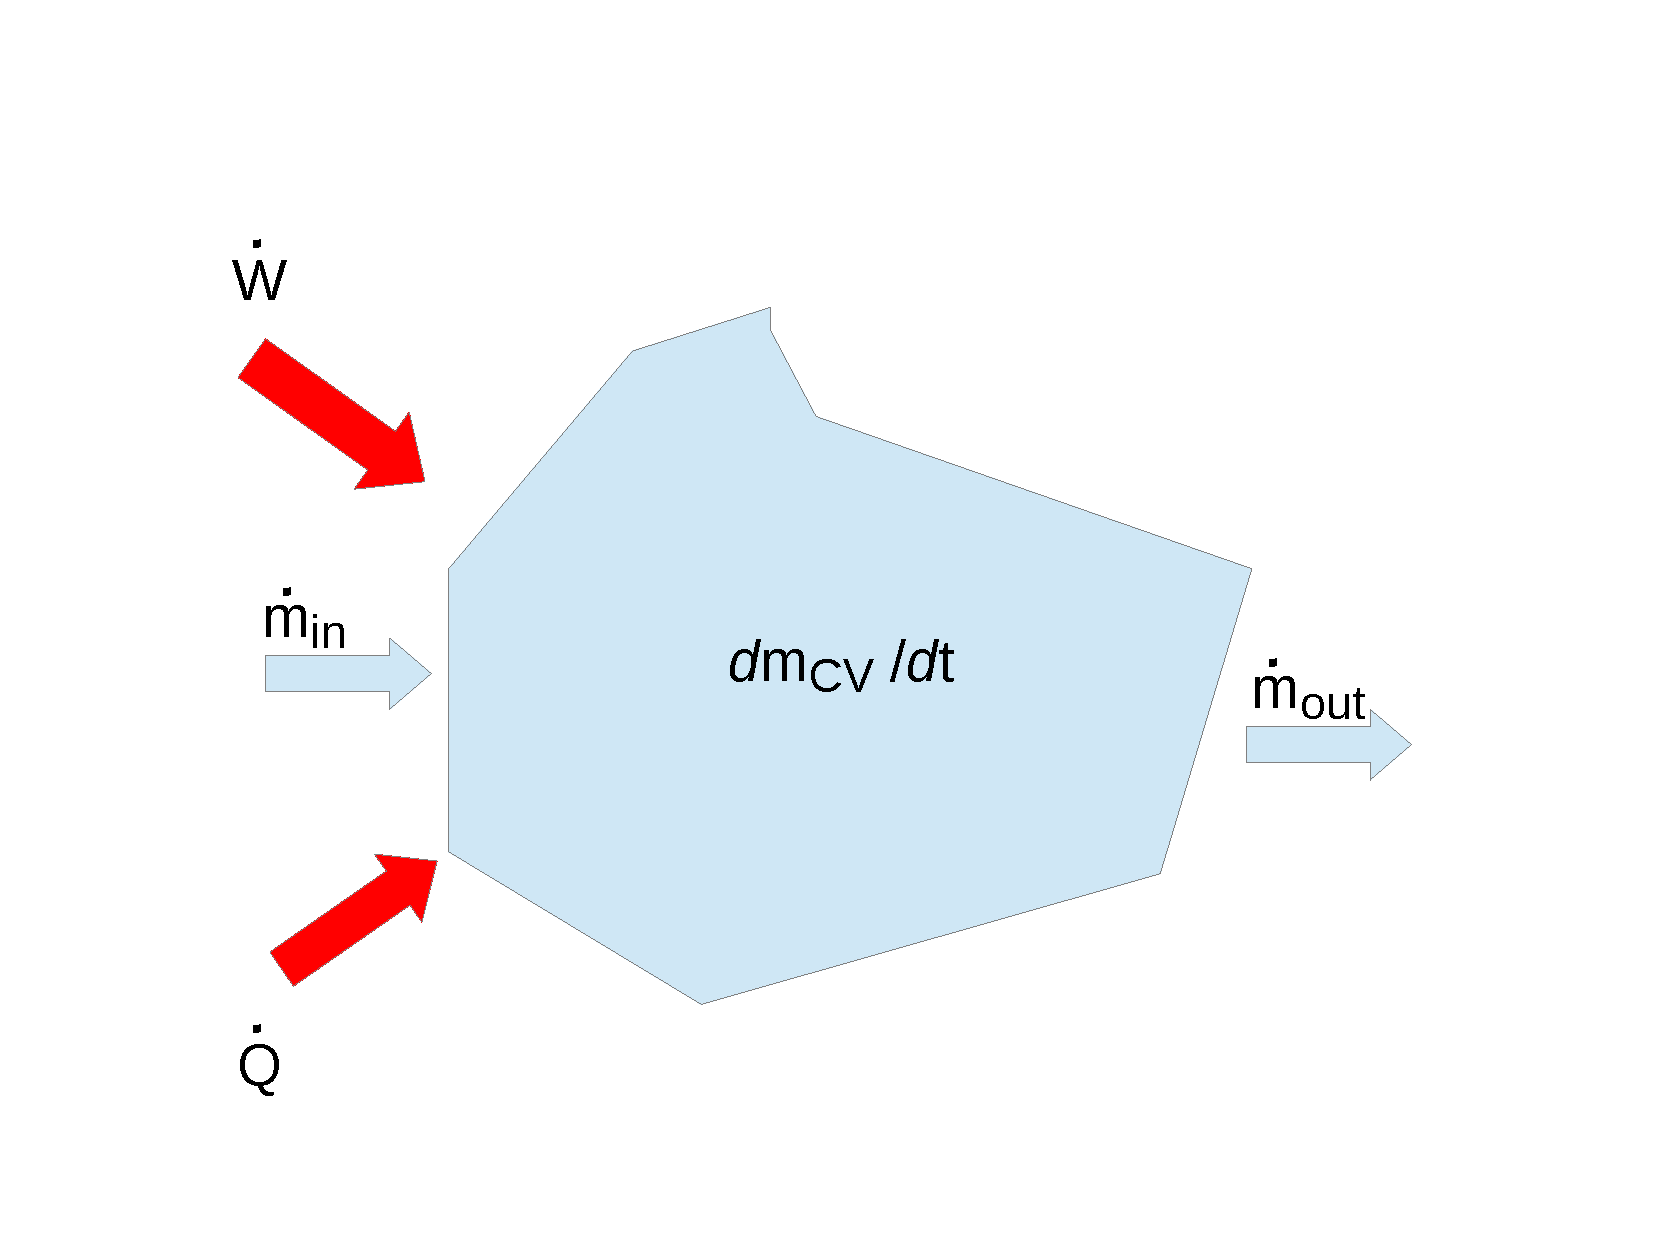
\includegraphics[width=6.cm,clip]{./../Pics/Energy_OpenedSystems}
         \end{center}}
        \item<2-> Mass balance:
             \visible<2->{\begin{displaymath}
                \frac{d m_{cv}}{dt}+ \left(\dot{m}_{out}-\dot{m}_{in}\right) = 0
             \end{displaymath}} 
     \end{itemize}
 
 \normalsize
\end{frame}

%%%
%%% Slides
%%%
\begin{frame}
 \frametitle{Open Systems}
     \begin{itemize}
        \item<1-> Energy balance:
           \visible<1->{\begin{displaymath}
             \frac{d\left(m U\right)_{cv}}{d t} + \Delta\left[\left(H + \frac{1}{2}u^{2} + z g\right)\dot{m}\right]=\dot{Q}+\dot{W}
           \end{displaymath}} 
        \item<2-> Steady-state flow process:
           \visible<2->{\begin{eqnarray}
             && \cancelto{0}{\frac{d\left(m U\right)_{cv}}{d t}} + \Delta\left[\left(H + \frac{1}{2}u^{2} + z g\right)\dot{m}\right]=\dot{Q}+\dot{W} \nonumber \\
             && \textcolor{blue}{\Delta H + \frac{\Delta u^{2}}{2} +g\Delta z= Q + W} \nonumber 
           \end{eqnarray}}          
     \end{itemize}
 
 \normalsize
\end{frame}


%%%
%%% SECTION
%%%
\subsection{Ideal Gas}

%%%
%%% Slides
%%%
\begin{frame}
 \frametitle{Ideal Gas: General Remarks}
     \begin{enumerate}
        \item<1-> Equation of state:
           \visible<1->{\begin{displaymath}
              P V = R T
           \end{displaymath}} 
        \item<2-> Heat capacity ratios:
           \visible<2->{\begin{eqnarray}
             && C_{V}=\left(\frac{\partial U}{\partial T}\right)_{V} = \frac{d U(T)}{d T} = C_{V}(T) \nonumber \\
             && C_{P}=\left(\frac{\partial H}{\partial T}\right)_{P} = \frac{d H(T)}{d T} = C_{P}(T) \nonumber
           \end{eqnarray}}    
        \item<3-> Internal energy {\bf depends only on} the temperature, $U = U(T)$;    
        \item<4-> Formally defining {\it Enthalpy}:
           \visible<4->{\begin{displaymath}
              H \equiv U + PV = U(T) + RT = H(T)
           \end{displaymath}} 
        \item<5-> Relationship between $C_{P}(T)$ and $C_{V}(T)$:
           \visible<5->{\begin{displaymath}
              \textcolor{red}{C_{P}}=\frac{d H(T)}{d T} = \frac{d U(T)}{d T} + \frac{d(RT)}{d T} = \textcolor{red}{C_{V} + R}
           \end{displaymath}}           
     \end{enumerate} 
  \normalsize
\end{frame}

%%%
%%% Slides
%%%
\begin{frame}
 \frametitle{Ideal Gas: Processes}
     \begin{enumerate}
        \item<1-> Processes involving {\it heat} and {\it work} quantities:
           \visible<1->{\begin{eqnarray}
             && d Q = C_{V} dT + RT \frac{d V}{V}  \Longleftrightarrow dW = -RT\frac{d V}{V} \nonumber \\
             && d Q = C_{P} dT - RT \frac{d P}{P}  \Longleftrightarrow dW = -R d T + RT\frac{d P}{P} \nonumber
           \end{eqnarray}} 
        \item<2-> With $PV = RT$
           \visible<2->{\begin{displaymath}
              d W = -P d V  \Longleftrightarrow dQ = \frac{C_{V}}{R}VdP + \frac{C_{P}}{R}P d V  
           \end{displaymath}}    
     \end{enumerate} 
  \normalsize
\end{frame}


%%%
%%% Slides
%%%
\begin{frame}
 \frametitle{Ideal Gas: Processes}
     \begin{enumerate}  \setcounter{enumi}{2}
        \item<1-> Isothermal procesess $(dT = 0)$:
           \visible<1->{\begin{displaymath}
              Q = -W = RT \ln\frac{V_{2}}{V_{1}} = -RT \ln\frac{P_{2}}{P_{1}}
           \end{displaymath}} 
        \item<2-> Isobaric process $(dP= 0)$:
           \visible<2->{\begin{displaymath}
              Q = \Delta H = \int\limits_{T_{1}}^{T_{2}}C_{P}dT
           \end{displaymath}}    
        \item<3-> Isochoric process $(dV= 0)$:
           \visible<3->{\begin{displaymath}
              Q = \Delta U = \int\limits_{T_{1}}^{T_{2}}C_{V}dT
           \end{displaymath}}     
     \end{enumerate} 
  \normalsize
\end{frame}


%%%
%%% Slides
%%%
\begin{frame}
 \frametitle{Ideal Gas: Processes}
     \begin{enumerate}  \setcounter{enumi}{5}
        \item<1-> Adiabatic process $(dQ= 0)$:
           \visible<1->{\begin{displaymath}
               \frac{T_{2}}{T_{1}} = \left(\frac{V_{1}}{V_{2}}\right)^{\frac{R}{C_{V}}} \Leftrightarrow \frac{T_{2}}{T_{1}} = \left(\frac{P_{2}}{P_{1}}\right)^{\frac{R}{C_{P}}} \Leftrightarrow \frac{P_{2}}{P_{1}} = \left(\frac{V_{1}}{V_{2}}\right)^{\frac{C_{P}}{C_{V}}} 
           \end{displaymath}}    
         \item<2-> If we define $\gamma \equiv \displaystyle\frac{C_{P}}{C_{V}}$, the relations above can be rewritten as,
           \visible<2->{\begin{displaymath}
               TV^{\gamma-1}=\text{const.} \Leftrightarrow TP^{\frac{1-\gamma}{\gamma}}=\text{const.} \Leftrightarrow PV^{\gamma}=\text{const.} 
           \end{displaymath}}    
         \item<3-> And for {\it polytropic} processes,
           \visible<3->{\begin{displaymath}
               TV^{\delta-1}=\text{const.} \Leftrightarrow TP^{\frac{1-\delta}{\delta}}=\text{const.} \Leftrightarrow PV^{\delta}=\text{const.} 
           \end{displaymath}}    
     \end{enumerate} 
  \normalsize
\end{frame}



%%%
%%%  SUBSECTION
%%%
\subsection{Statements of the Second Law}

%%%
%%% Slides
%%%
\begin{frame}
 \frametitle{Second Law of Thermodynamics}
 %\scriptsize
 \begin{itemize}
   \item <2->The second law of thermodynamics is an expression of the tendency that over time, differences in temperature, pressure and chemical potential will reach an equilibrium state in an isolated physical system;
   \item <3->From the state of thermodynamic equilibrium, the law deduced the principle of the increase of entropy and explains the phenomenon of irreversibility.
 \end{itemize}

 \visible<4->{\begin{block}{R. Clausius  (1854)}
  \begin{center}
  \textcolor{blue}{$\lq$It is impossible to devise an engine which, working in a cycle, shall produce no effect other than the transfer of heat from a colder to hotter body.'}
  \end{center}
 \end{block}}

 \visible<5->{\begin{block}{Kelvin (1951) and Planck (1897)}
  \begin{center}
  \textcolor{blue}{$\lq$It is impossible to devise an engine which, working in a cycle, shall produce no effect other than the extraction of heat from a reservoir and the performance of an equal amount of mechanical work.'}
  \end{center}
 \end{block}}

 \normalsize
\end{frame}


%%%
%%% Slides
%%%
\begin{frame}
 \frametitle{Second Law of Thermodynamics}
 
   \begin{figure}%
    \begin{center}
     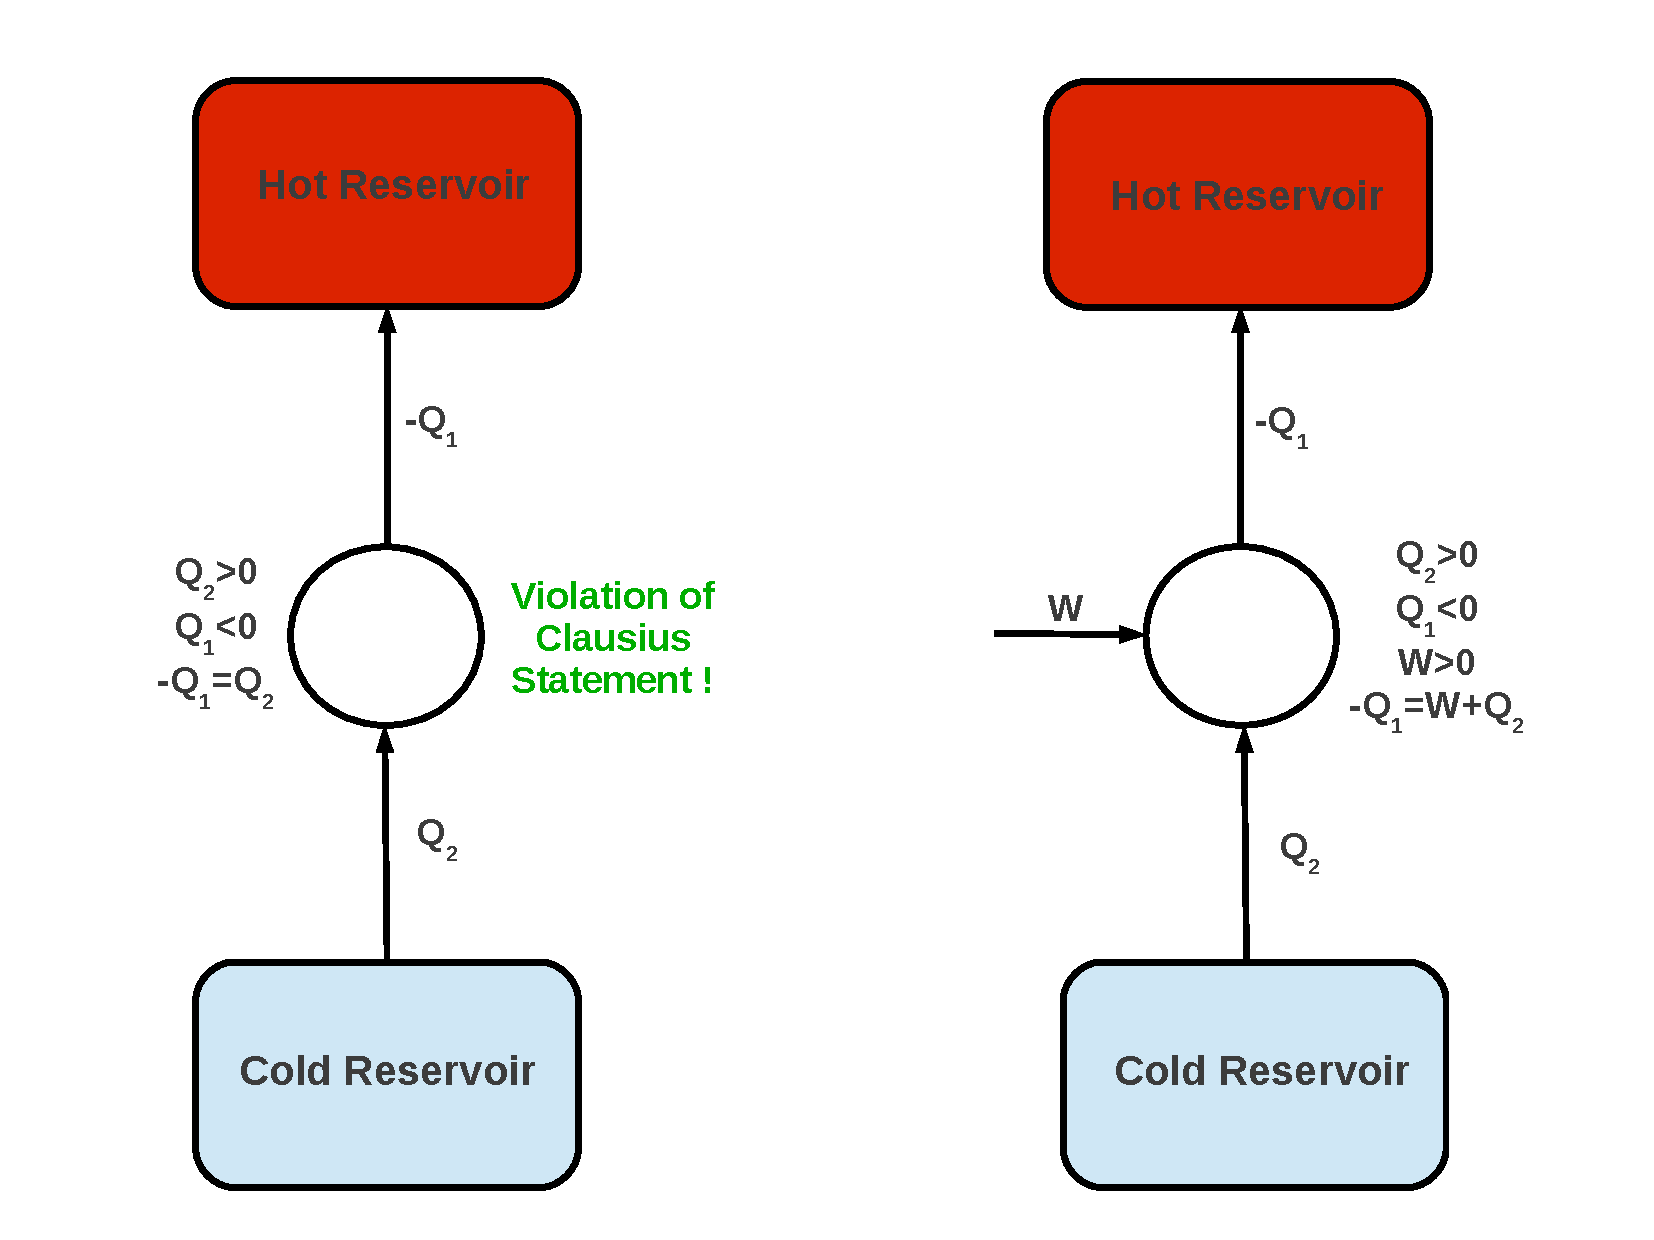
\includegraphics[width=8.cm,clip]{./../Pics/2ndLaw_Schem}
    \end{center}
   \end{figure} 

   \begin{center}
     All spontaneous processes are irreversible -- heat flows from hot to cold spontaneously and irreversibly.
   \end{center}
   
\end{frame}

%%%
%%% Slides
%%%
\begin{frame}
 \frametitle{Second Law of Thermodynamics}
     \begin{block}{\begin{center}Mathematical Representation of the 2$^{\text{nd}}$ Law\end{center}}
        \visible<1->{\begin{eqnarray}
            \textcolor{blue}{\displaystyle\oint \displaystyle\frac{d Q}{T} < 0 \;\;\; \text{for irreversible processes}} \nonumber \\
            \textcolor{blue}{\displaystyle\oint \displaystyle\frac{d Q}{T} = 0 \;\;\;\;\; \text{for reversible processes}} \nonumber 
        \end{eqnarray}}
     \end{block}

\visible<2->{\begin{block}{\begin{center}{\bf Entropy} \end{center}}
           \begin{displaymath}
              dS = \left( \frc{d Q}{T}\right)_{\text{int. rev.}}\hspace{3cm}\left(\frc{J}{kg.K}\right)
           \end{displaymath}
\end{block}}
   
\end{frame}

%%%
%%% COMMENTS
%%%
\begin{comment}

%%%
%%% Slides
%%%
\begin{frame}
 \frametitle{Derivation of the Mathematical Statement of the Second Law}
 %\scriptsize
 \begin{columns}

  \begin{column}[c]{0.5\linewidth}
   \begin{itemize}
    \item <2-> In the schematics (rhs), an infinitesimal amount of heat, $\delta Q^{\prime}$, is transferred from the thermal reservoir (with temperature $T_{res}$) to a reversible cyclic engine (1). 
    \item <3-> The engine produces a small amount of work, $\delta W^{\prime}$, and releases an infinitesimal amount of heat, $\delta Q$ to another reservoir at variable temperature $T$. 
    \item <4-> The second reservoir (2) also releases work $\left(\delta W\right)$ to the surroundings.
   \end{itemize}


  \end{column}

  \begin{column}[c]{0.5\linewidth}
   \begin{figure}%
    \begin{center}
     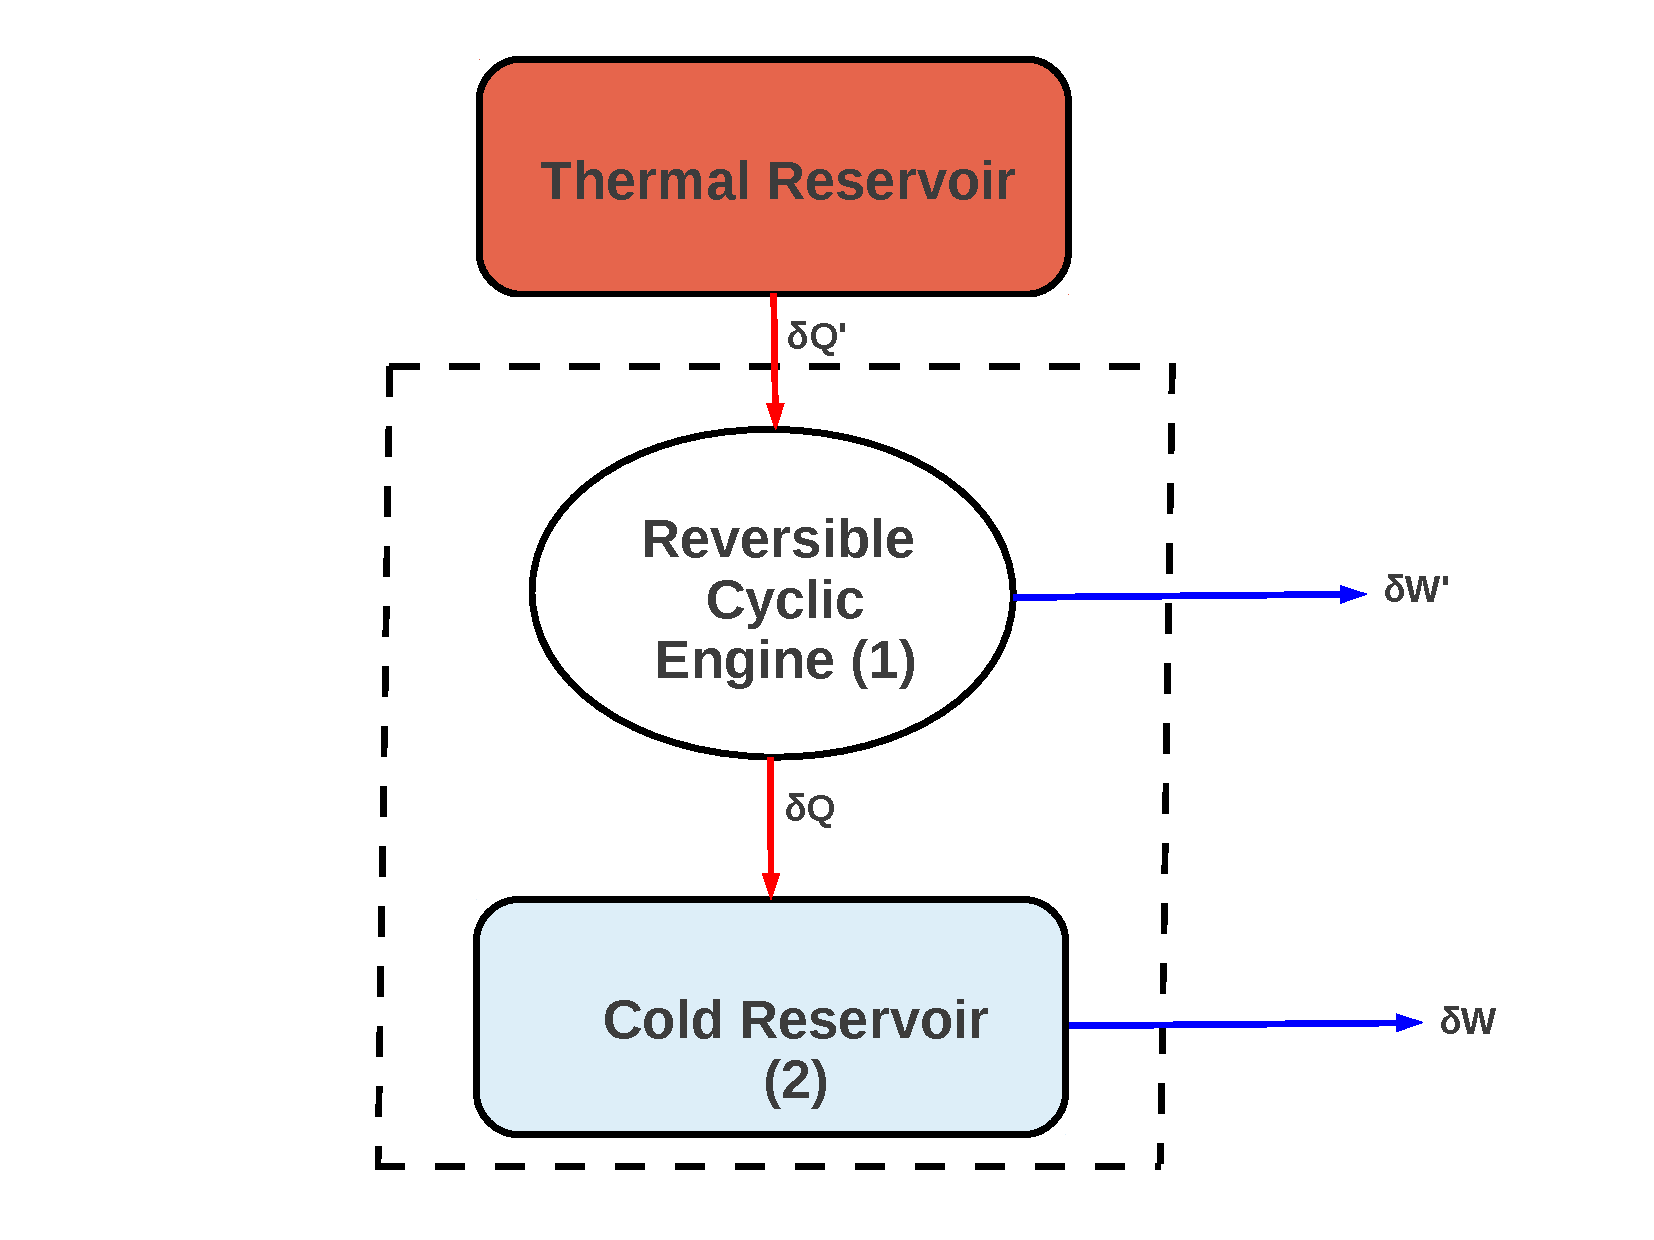
\includegraphics[width=1.1\columnwidth,clip]{./../Pics/2ndLaw_Schem2}
    \end{center}
   \end{figure} 
  \end{column}
 \end{columns}


 \normalsize
    
\end{frame}

%%%
%%% Slides
%%%
\begin{frame}
 \frametitle{Derivation of the Mathematical Statement of the Second Law}
 %\scriptsize
 \begin{columns}

  \begin{column}[c]{0.5\linewidth}
   \begin{itemize}
    \item <1-> Using the analogy of heat transfer ratio and temperature ratio (see power cycle systems), \\
                $\displaystyle\frac{\delta Q^{\prime}}{\delta Q} = \displaystyle\frac{T_{res}}{T} \;\; \Longrightarrow \displaystyle\frac{\delta Q^{\prime}}{T_{res}} = \displaystyle\frac{\delta Q}{T}$
  \item <2-> The first law in differential form for the combined cycle (within the dotted box) is \\
                $dU= \delta Q^{\prime} - \left(\delta W + \delta W^{\prime}\right) \Longrightarrow \delta W + \delta W^{\prime} = \delta Q^{\prime} - dU$
  \item <3-> The process is not required to be cyclic and the heat transfer $\delta Q$ is internal and do not cross the boundary of the combined system;
   \end{itemize}


  \end{column}

  \begin{column}[c]{0.5\linewidth}
   \begin{figure}%
    \begin{center}
     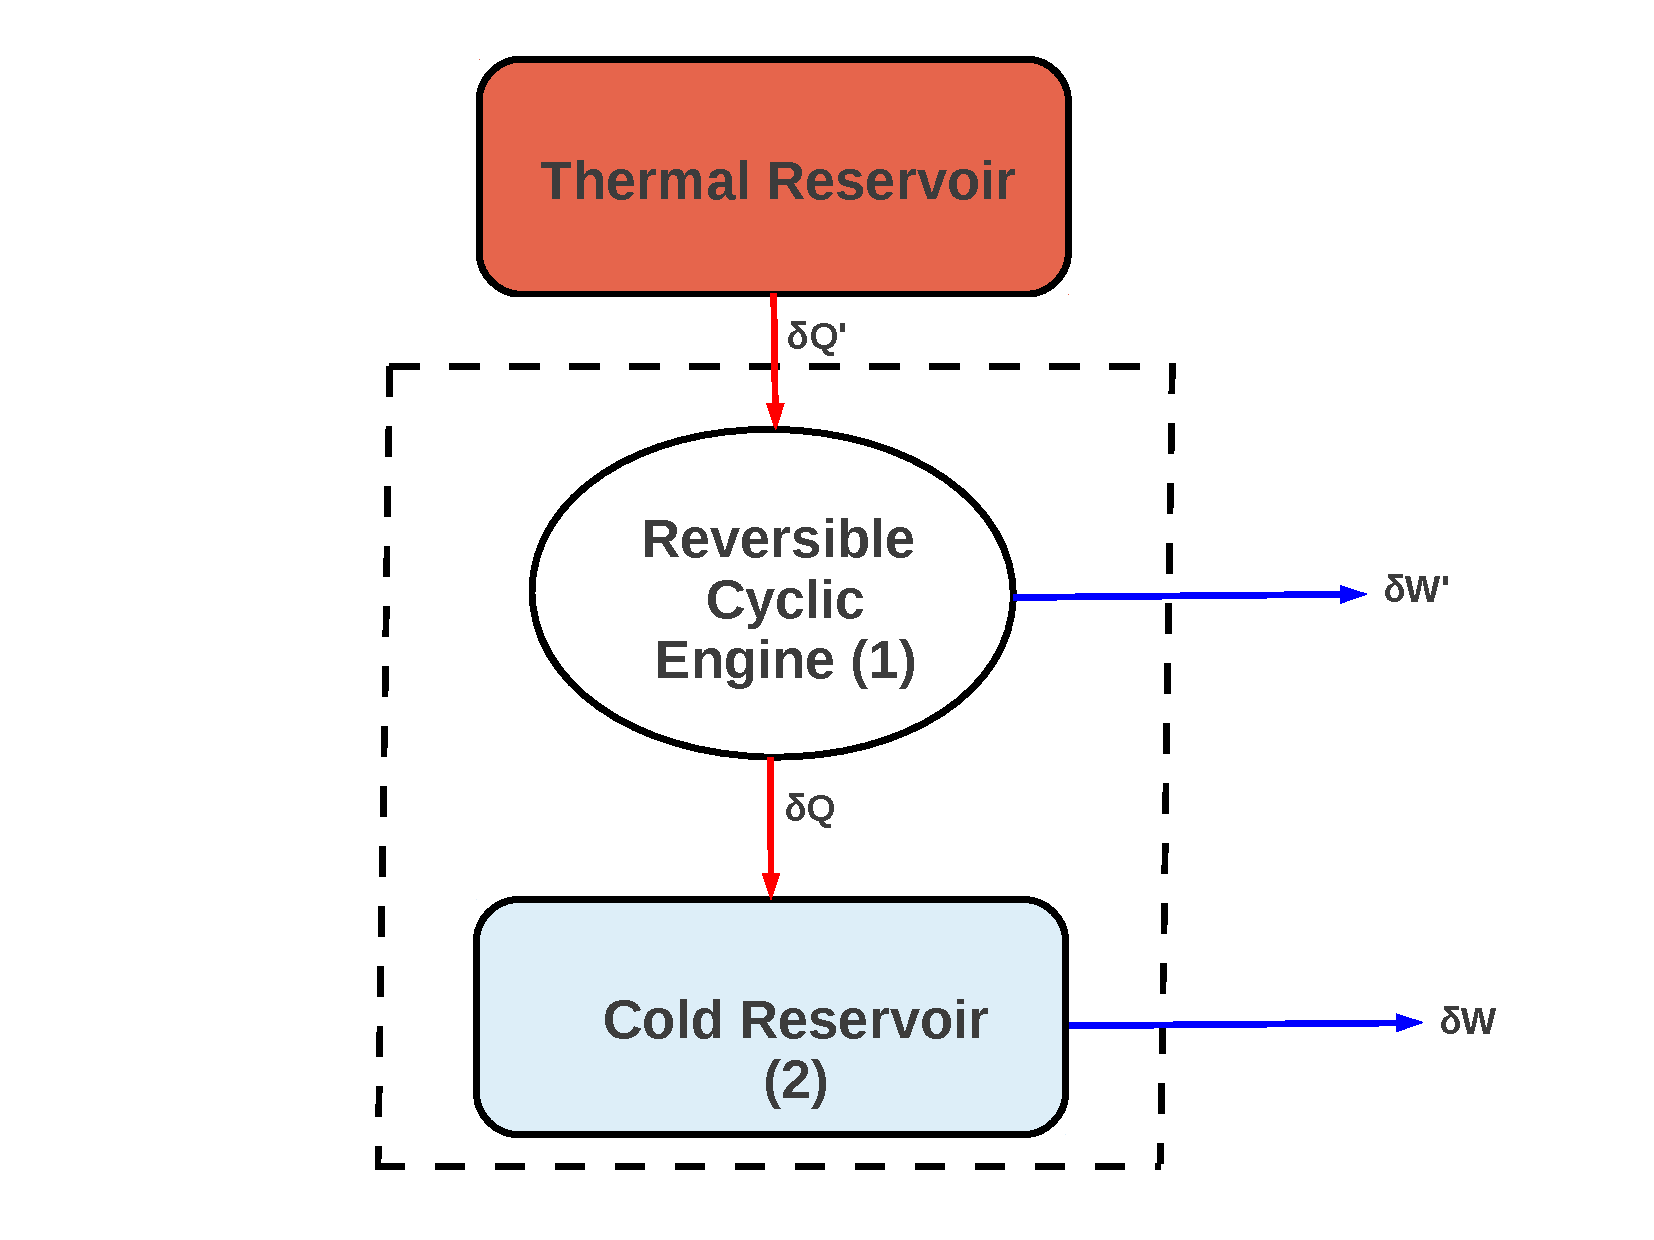
\includegraphics[width=1.1\columnwidth,clip]{./../Pics/2ndLaw_Schem2}
    \end{center}
   \end{figure} 
  \end{column}
 \end{columns}
 \normalsize
    
\end{frame}


%%%
%%% Slides
%%%
\begin{frame}
 \frametitle{Derivation of the Mathematical Statement of the Second Law}
 %\scriptsize
 \begin{columns}

  \begin{column}[c]{0.5\linewidth}
   \begin{itemize}
    \item <1-> And eliminating $\delta Q^{\prime}$, \\
                $\delta W + \delta W^{\prime} = T_{res}\displaystyle\frac{\delta Q}{T} - dU$
     \item <2-> If the configuration shown in the previous slide undergoes a cyclic process, \\
             $\displaystyle\oint \delta W + \displaystyle\oint \delta W^{\prime} = \displaystyle\oint T_{res}\displaystyle\frac{\delta Q}{T} - \displaystyle\oint dU$
     \item <3-> as $U$ is a thermodynamic property, the cyclic integral is equal to zero.  Integrating the equation above, and assuming that $T_{res}$ is (by definition) constant:\\
             $W + W^{\prime} = T_{res} \displaystyle\oint \displaystyle\frac{\delta Q}{T}$
   \end{itemize}
  \end{column}

  \begin{column}[c]{0.5\linewidth}
   \begin{figure}%
    \begin{center}
     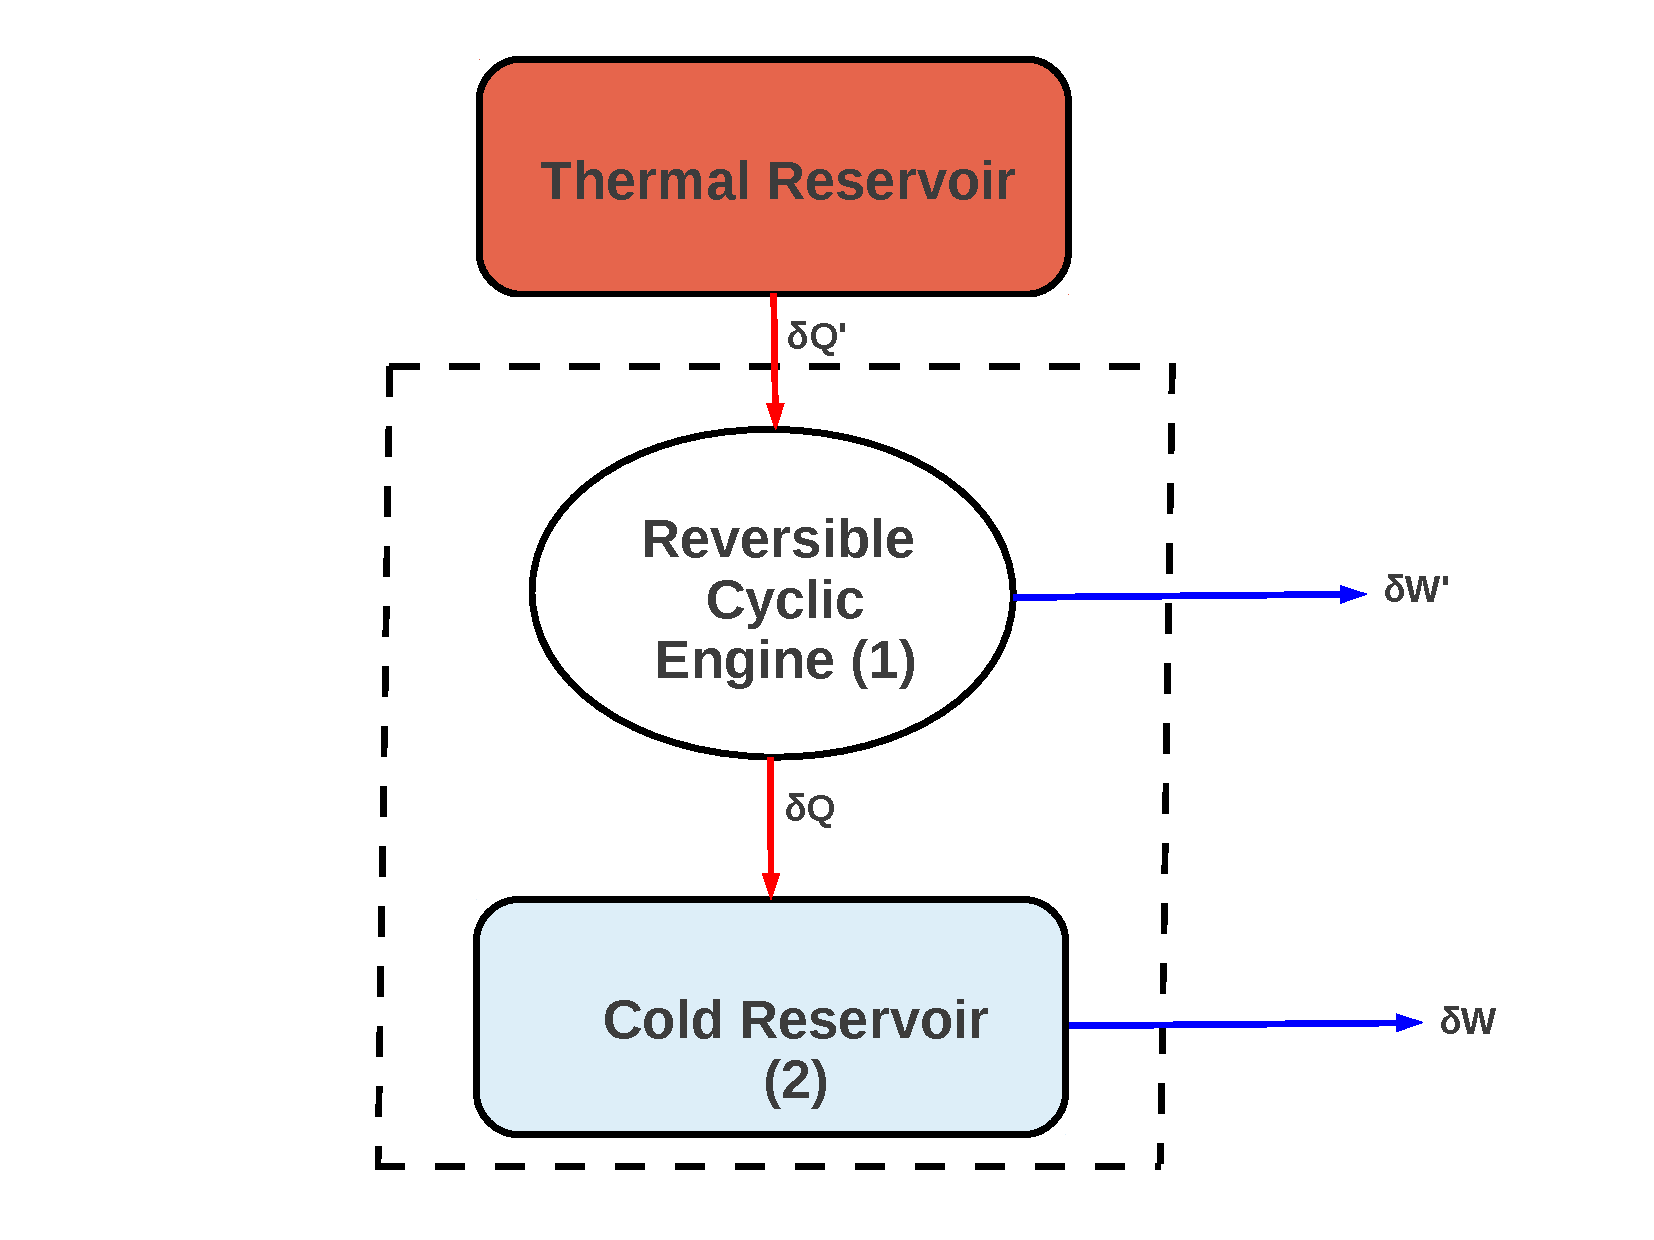
\includegraphics[width=1.1\columnwidth,clip]{./../Pics/2ndLaw_Schem2}
    \end{center}
   \end{figure} 
  \end{column}
 \end{columns}
 \normalsize
    
\end{frame}


%%%
%%% Slides
%%%
\begin{frame}
 \frametitle{Derivation of the Mathematical Statement of the Second Law}
   \begin{itemize}
    \item <1-> Thus from Kelvin-Plancks statement of the Second Law -- \textcolor{blue}{$\lq$we cannot convert all the heat to work, but we can convert all the work to heat'}:\\
             $W + W^{\prime} \leq 0$
    \item <2-> And therefore,\\
             $T_{res} \displaystyle\displaystyle\oint \displaystyle\frac{\delta Q}{T} \leq 0$
    \item <3->  Since $T_{res} > 0$, we can divide the previous equation without changing the meaning of the inequality to obtain the mathematical representation of the Second Law:
             \begin{eqnarray}
             \textcolor{blue}{\displaystyle\oint \displaystyle\frac{\delta Q}{T} < 0 \;\;\; \text{for irreversible processes}} \nonumber \\
             \textcolor{blue}{\displaystyle\oint \displaystyle\frac{\delta Q}{T} = 0 \;\;\;\;\; \text{for reversible processes}} \nonumber 
             \end{eqnarray}
   \end{itemize}
 \normalsize
\end{frame}


%%%
%%% Slides
%%%
\begin{frame}
 \frametitle{Derivation of the Mathematical Statement of the Second Law}
   \begin{itemize}
    \item <1-> In a reversible process, from state 1 to 2, via path {\it A}, and returning to state 2 from either path {\it B} or {\it C}. The cyclic integral $\displaystyle\oint\displaystyle\frac{\delta Q}{T} = 0$ can be split as,
         \textcolor{blue}{\begin{eqnarray}
          \left( \displaystyle\int\limits_{1}^{2} \displaystyle\frac{\delta Q}{T} \right)_{A} + \left( \displaystyle\int\limits_{2}^{1} \displaystyle\frac{\delta Q}{T} \right)_{B} = 0 \nonumber \\
          \left( \displaystyle\int\limits_{1}^{2} \displaystyle\frac{\delta Q}{T} \right)_{A} + \left( \displaystyle\int\limits_{2}^{1} \displaystyle\frac{\delta Q}{T} \right)_{C} = 0 \nonumber 
         \end{eqnarray}}
   \end{itemize}
 \normalsize
    
\end{frame}

%%%
%%% Slides
%%%
\begin{frame}
 \frametitle{Derivation of the Mathematical Statement of the Second Law}
   \begin{itemize}
    \item <2-> Leading to:
          $\left( \displaystyle\int\limits_{1}^{2} \displaystyle\frac{\delta Q}{T} \right)_{B} = \left( \displaystyle\int\limits_{2}^{1} \displaystyle\frac{\delta Q}{T} \right)_{C} $
    \item <3-> Since paths {\it B} and {\it C} are different and arbitrary, but $\displaystyle\int\limits_{1}^{2}\displaystyle\frac{\delta Q}{T}$ is the same on either paths -- therefore \textcolor{blue}{the integral is path-independent};
    \item <4-> This defines another (extensive) thermodynamic property -- \textcolor{red}{entropy (S)}, \\
          $S_{2} - S_{1} = \displaystyle\int\limits_{1}^{2}\displaystyle\frac{\delta Q}{T}$
    \item <5-> Assuming constant mass ($m$), the intensive property entropy $\left(s=S/m\right)$, the differential form is, \\
          $ds = \displaystyle\frac{\delta q}{T} \;\;\;\; \Longrightarrow \;\;\;\; \delta q = Tds$
    \item <6-> Integrating from state 1 to 2: $q_{1}^{2} = \displaystyle\int_{1}^{2} Tds$    
   \end{itemize}
 \normalsize
\end{frame}


%%%
%%% Slides
%%%
\begin{frame}
 \frametitle{Derivation of the Mathematical Statement of the Second Law}
   \begin{itemize}
  \item <1-> This is the heat transfer equivalent of $w_{1}^{2}=\displaystyle\int_{1}^{2}PdV$
  \item <2-> Thus for a reversible process, \\
       $S_{2} - S_{1} = \displaystyle\int\limits_{1}^{2}\displaystyle\frac{\delta Q}{T}$ and $S_{1} - S_{2} = \displaystyle\int\limits_{2}^{1}\displaystyle\frac{\delta Q}{T}$;
  \item <3-> From the Second Law, \\
       $0 \geq \left( \displaystyle\int\limits_{1}^{2}\displaystyle\frac{\delta Q}{T} \right)_{A} + \left( \displaystyle\int\limits_{2}^{1}\displaystyle\frac{\delta Q}{T} \right)_{B}$ 
  \item <4-> Combinig the equations above to eliminate the path {\it B}, \\
        $S_{2}-S_{1} \geq \displaystyle\int\limits_{1}^{2}\displaystyle\frac{\delta Q}{T}$
 \end{itemize}
 \normalsize
\end{frame}


%%%
%%% Slides
%%%
\begin{frame}
 \frametitle{Derivation of the Mathematical Statement of the Second Law}
   \begin{itemize}
  \item <1-> If path {\it A} is reversible, the equality holds, however if {\it A} is irreversible, the inequality holds;
  \item <2-> If the system is isolated $\left(\delta Q = 0\right)$ then\\
    $S_{2}-S_{1}\geq 0$
   \end{itemize}
 \normalsize
    
\end{frame}

%%%
%%% END OF COMMENTED TEXT
%%%
\end{comment}


%%%
%%% SUBSECTION
%%%
\subsection{Entropy} 

%%%
%%% Slides
%%%
\begin{frame}
 \frametitle{Ideal Gas}
   \begin{enumerate}
     \item<1-> Mechanically reversible process of closed system
        \visible<1->{\begin{displaymath}
           dU = dQ_{\text{rev}} - PdV
        \end{displaymath}}
     \item<2-> Applying the definition of entropy and enthalpy,
        \visible<2->{\begin{displaymath}
           \displaystyle\frac{\Delta S}{R} = \int\limits_{T_{0}}^{T}\displaystyle\frac{C_{p}^{\text{ig}}}{R}\displaystyle\frac{d T}{T} - \ln\displaystyle\frac{P}{P_{0}}
        \end{displaymath}}
     \item<2-> This relates {\bf only} to \textcolor{blue}{properties}, i.e., \textcolor{blue}{independent of the process}.
   \end{enumerate}
 \normalsize
\end{frame}





\section{Summary}
%%%
%%% Slides
%%%
\begin{frame}
 \frametitle{Summary}
After these set of lectures you should know the fundamentals of thermodynamics which will be relevant to understand heat-engine cycles. This includes knowledge of: 
 \begin{enumerate}[(a)]
  \item <2-> Phase diagram and steam tables;
  \item <3-> Zeroth, First and Second laws;
  \item <4-> Reversibility and its impact on thermodynamics formulation;
  \item <5-> Definition of the key thermodynamic properties, e.g., work, heat, temperature, internal energy, enthalpy, entropy, etc;
  \item <6-> Mass and energy balances in open and closed systems.
 \end{enumerate}
\end{frame}

 
%%%
%%% Appendix
%%%
%\subsection{Appendix}
%\begin{frame}
%\begin{itemize}
%\item Saturated Water and Steam Tables;
%\item Superheated Steam at Various Pressure and Temperatures;
%\item Units Conversion.
%\end{itemize}
%\end{frame}


%{
%  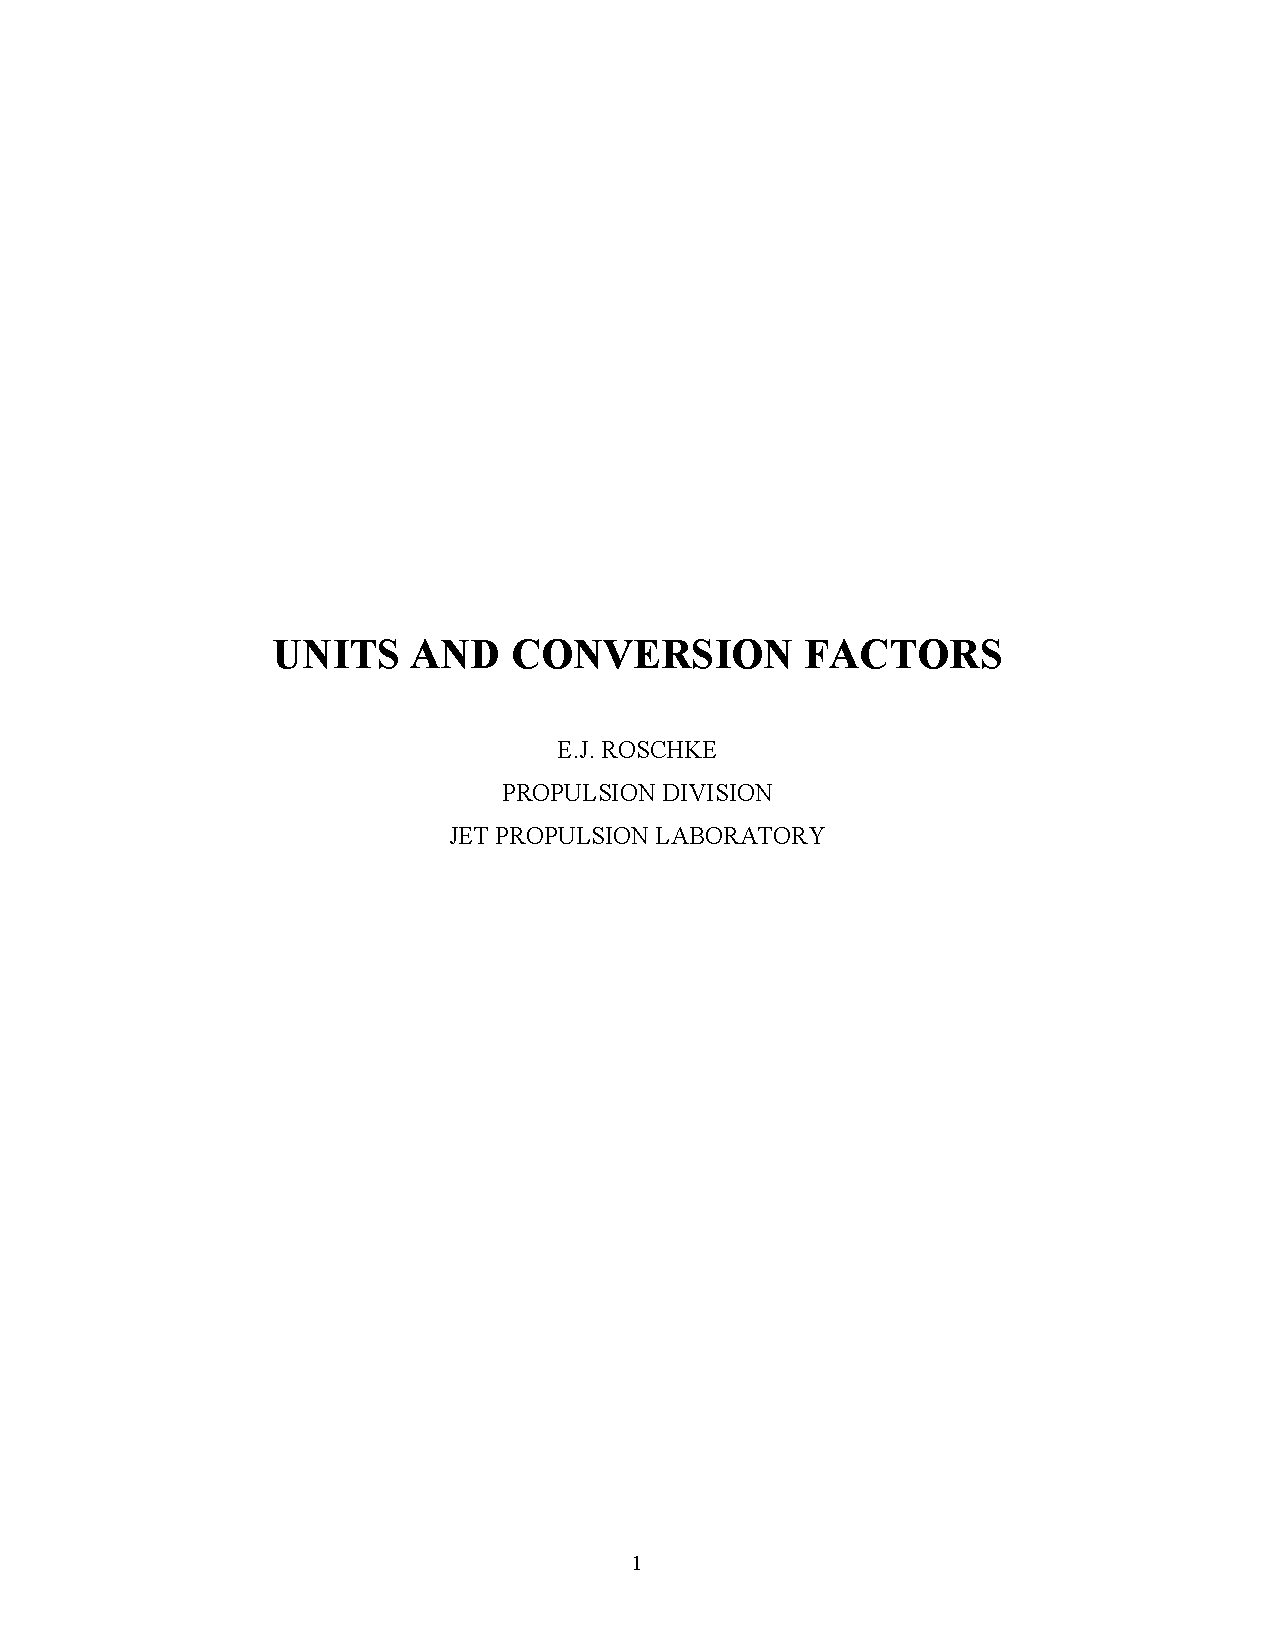
\includepdf[pages=-,fitpaper]{./../Pics/Roschke.pdf}
%}


\end{document}
